\documentclass[twoside]{book}

% Packages required by doxygen
\usepackage{fixltx2e}
\usepackage{calc}
\usepackage{doxygen}
\usepackage[export]{adjustbox} % also loads graphicx
\usepackage{graphicx}
\usepackage[utf8]{inputenc}
\usepackage{makeidx}
\usepackage{multicol}
\usepackage{multirow}
\PassOptionsToPackage{warn}{textcomp}
\usepackage{textcomp}
\usepackage[nointegrals]{wasysym}
\usepackage[table]{xcolor}

% Font selection
\usepackage[T1]{fontenc}
\usepackage[scaled=.90]{helvet}
\usepackage{courier}
\usepackage{amssymb}
\usepackage{sectsty}
\renewcommand{\familydefault}{\sfdefault}
\allsectionsfont{%
  \fontseries{bc}\selectfont%
  \color{darkgray}%
}
\renewcommand{\DoxyLabelFont}{%
  \fontseries{bc}\selectfont%
  \color{darkgray}%
}
\newcommand{\+}{\discretionary{\mbox{\scriptsize$\hookleftarrow$}}{}{}}

% Page & text layout
\usepackage{geometry}
\geometry{%
  a4paper,%
  top=2.5cm,%
  bottom=2.5cm,%
  left=2.5cm,%
  right=2.5cm%
}
\tolerance=750
\hfuzz=15pt
\hbadness=750
\setlength{\emergencystretch}{15pt}
\setlength{\parindent}{0cm}
\setlength{\parskip}{0.2cm}
\makeatletter
\renewcommand{\paragraph}{%
  \@startsection{paragraph}{4}{0ex}{-1.0ex}{1.0ex}{%
    \normalfont\normalsize\bfseries\SS@parafont%
  }%
}
\renewcommand{\subparagraph}{%
  \@startsection{subparagraph}{5}{0ex}{-1.0ex}{1.0ex}{%
    \normalfont\normalsize\bfseries\SS@subparafont%
  }%
}
\makeatother

% Headers & footers
\usepackage{fancyhdr}
\pagestyle{fancyplain}
\fancyhead[LE]{\fancyplain{}{\bfseries\thepage}}
\fancyhead[CE]{\fancyplain{}{}}
\fancyhead[RE]{\fancyplain{}{\bfseries\leftmark}}
\fancyhead[LO]{\fancyplain{}{\bfseries\rightmark}}
\fancyhead[CO]{\fancyplain{}{}}
\fancyhead[RO]{\fancyplain{}{\bfseries\thepage}}
\fancyfoot[LE]{\fancyplain{}{}}
\fancyfoot[CE]{\fancyplain{}{}}
\fancyfoot[RE]{\fancyplain{}{\bfseries\scriptsize Generated on Mon Mar 9 2015 15\+:14\+:07 for Py\+Spinor by Doxygen }}
\fancyfoot[LO]{\fancyplain{}{\bfseries\scriptsize Generated on Mon Mar 9 2015 15\+:14\+:07 for Py\+Spinor by Doxygen }}
\fancyfoot[CO]{\fancyplain{}{}}
\fancyfoot[RO]{\fancyplain{}{}}
\renewcommand{\footrulewidth}{0.4pt}
\renewcommand{\chaptermark}[1]{%
  \markboth{#1}{}%
}
\renewcommand{\sectionmark}[1]{%
  \markright{\thesection\ #1}%
}

% Indices & bibliography
\usepackage{natbib}
\usepackage[titles]{tocloft}
\setcounter{tocdepth}{3}
\setcounter{secnumdepth}{5}
\makeindex

% Hyperlinks (required, but should be loaded last)
\usepackage{ifpdf}
\ifpdf
  \usepackage[pdftex,pagebackref=true]{hyperref}
\else
  \usepackage[ps2pdf,pagebackref=true]{hyperref}
\fi
\hypersetup{%
  colorlinks=true,%
  linkcolor=blue,%
  citecolor=blue,%
  unicode%
}

% Custom commands
\newcommand{\clearemptydoublepage}{%
  \newpage{\pagestyle{empty}\cleardoublepage}%
}


%===== C O N T E N T S =====

\begin{document}

% Titlepage & ToC
\hypersetup{pageanchor=false,
             bookmarks=true,
             bookmarksnumbered=true,
             pdfencoding=unicode
            }
\pagenumbering{roman}
\begin{titlepage}
\vspace*{7cm}
\begin{center}%
{\Large Py\+Spinor \\[1ex]\large 0.\+5 }\\
\vspace*{1cm}
{\large Generated by Doxygen 1.8.9.1}\\
\vspace*{0.5cm}
{\small Mon Mar 9 2015 15:14:07}\\
\end{center}
\end{titlepage}
\clearemptydoublepage
\tableofcontents
\clearemptydoublepage
\pagenumbering{arabic}
\hypersetup{pageanchor=true}

%--- Begin generated contents ---
\chapter{Namespace Index}
\section{Packages}
Here are the packages with brief descriptions (if available)\+:\begin{DoxyCompactList}
\item\contentsline{section}{\hyperlink{namespace_py_spinor}{Py\+Spinor} }{\pageref{namespace_py_spinor}}{}
\item\contentsline{section}{\hyperlink{namespace_py_spinor_1_1_colour}{Py\+Spinor.\+Colour} }{\pageref{namespace_py_spinor_1_1_colour}}{}
\item\contentsline{section}{\hyperlink{namespace_py_spinor_1_1_common}{Py\+Spinor.\+Common} }{\pageref{namespace_py_spinor_1_1_common}}{}
\item\contentsline{section}{\hyperlink{namespace_py_spinor_1_1_current}{Py\+Spinor.\+Current} }{\pageref{namespace_py_spinor_1_1_current}}{}
\item\contentsline{section}{\hyperlink{namespace_py_spinor_1_1_gluon}{Py\+Spinor.\+Gluon} }{\pageref{namespace_py_spinor_1_1_gluon}}{}
\item\contentsline{section}{\hyperlink{namespace_py_spinor_1_1_lorentz_vector}{Py\+Spinor.\+Lorentz\+Vector} }{\pageref{namespace_py_spinor_1_1_lorentz_vector}}{}
\item\contentsline{section}{\hyperlink{namespace_py_spinor_1_1_momenta}{Py\+Spinor.\+Momenta} }{\pageref{namespace_py_spinor_1_1_momenta}}{}
\item\contentsline{section}{\hyperlink{namespace_py_spinor_1_1pol_dictionary}{Py\+Spinor.\+pol\+Dictionary} }{\pageref{namespace_py_spinor_1_1pol_dictionary}}{}
\item\contentsline{section}{\hyperlink{namespace_py_spinor_1_1_spinor}{Py\+Spinor.\+Spinor} }{\pageref{namespace_py_spinor_1_1_spinor}}{}
\item\contentsline{section}{\hyperlink{namespace_py_spinor_1_1spinor_string}{Py\+Spinor.\+spinor\+String} }{\pageref{namespace_py_spinor_1_1spinor_string}}{}
\item\contentsline{section}{\hyperlink{namespace_py_spinor_1_1_spinor_tensor}{Py\+Spinor.\+Spinor\+Tensor} }{\pageref{namespace_py_spinor_1_1_spinor_tensor}}{}
\item\contentsline{section}{\hyperlink{namespace_py_spinor_1_1_tensor}{Py\+Spinor.\+Tensor} }{\pageref{namespace_py_spinor_1_1_tensor}}{}
\item\contentsline{section}{\hyperlink{namespace_py_spinor_1_1_utility}{Py\+Spinor.\+Utility} }{\pageref{namespace_py_spinor_1_1_utility}}{}
\end{DoxyCompactList}

\chapter{Hierarchical Index}
\section{Class Hierarchy}
This inheritance list is sorted roughly, but not completely, alphabetically\+:\begin{DoxyCompactList}
\item object\begin{DoxyCompactList}
\item \contentsline{section}{Py\+Spinor.\+Gluon.\+Gluon}{\pageref{class_py_spinor_1_1_gluon_1_1_gluon}}{}
\item \contentsline{section}{Py\+Spinor.\+Lorentz\+Vector.\+Lorentz\+Vector}{\pageref{class_py_spinor_1_1_lorentz_vector_1_1_lorentz_vector}}{}
\item \contentsline{section}{Py\+Spinor.\+pol\+Dictionary.\+pol\+Dictionary}{\pageref{class_py_spinor_1_1pol_dictionary_1_1pol_dictionary}}{}
\item \contentsline{section}{Py\+Spinor.\+Spinor.\+Spinor}{\pageref{class_py_spinor_1_1_spinor_1_1_spinor}}{}
\item \contentsline{section}{Py\+Spinor.\+spinor\+String.\+spinor\+String}{\pageref{class_py_spinor_1_1spinor_string_1_1spinor_string}}{}
\item \contentsline{section}{Py\+Spinor.\+Tensor.\+Tensor}{\pageref{class_py_spinor_1_1_tensor_1_1_tensor}}{}
\end{DoxyCompactList}
\item \contentsline{section}{Py\+Spinor.\+Spinor.\+Spinor.\+spinor}{\pageref{class_py_spinor_1_1_spinor_1_1_spinor_1_1spinor}}{}
\item \contentsline{section}{Py\+Spinor.\+Spinor\+Tensor.\+Spinor\+Tensor.\+tensor}{\pageref{class_py_spinor_1_1_spinor_tensor_1_1_spinor_tensor_1_1tensor}}{}
\item Lorentz\+Vector\begin{DoxyCompactList}
\item \contentsline{section}{Py\+Spinor.\+Current.\+Current.\+current}{\pageref{class_py_spinor_1_1_current_1_1_current_1_1current}}{}
\item \contentsline{section}{Py\+Spinor.\+Momenta.\+Momenta}{\pageref{class_py_spinor_1_1_momenta_1_1_momenta}}{}
\end{DoxyCompactList}
\item pol\+Dictionary\begin{DoxyCompactList}
\item \contentsline{section}{Py\+Spinor.\+Current.\+Current}{\pageref{class_py_spinor_1_1_current_1_1_current}}{}
\item \contentsline{section}{Py\+Spinor.\+Spinor\+Tensor.\+Spinor\+Tensor}{\pageref{class_py_spinor_1_1_spinor_tensor_1_1_spinor_tensor}}{}
\end{DoxyCompactList}
\end{DoxyCompactList}

\chapter{Class Index}
\section{Class List}
Here are the classes, structs, unions and interfaces with brief descriptions\+:\begin{DoxyCompactList}
\item\contentsline{section}{\hyperlink{class_py_spinor_1_1_current_1_1_current}{Py\+Spinor.\+Current.\+Current} \\*Class storing spinor current information }{\pageref{class_py_spinor_1_1_current_1_1_current}}{}
\item\contentsline{section}{\hyperlink{class_py_spinor_1_1_current_1_1_current_1_1current}{Py\+Spinor.\+Current.\+Current.\+current} \\*Lorentz vector currents }{\pageref{class_py_spinor_1_1_current_1_1_current_1_1current}}{}
\item\contentsline{section}{\hyperlink{class_py_spinor_1_1_gluon_1_1_gluon}{Py\+Spinor.\+Gluon.\+Gluon} \\*\hyperlink{class_py_spinor_1_1_gluon_1_1_gluon}{Gluon} class }{\pageref{class_py_spinor_1_1_gluon_1_1_gluon}}{}
\item\contentsline{section}{\hyperlink{class_py_spinor_1_1_lorentz_vector_1_1_lorentz_vector}{Py\+Spinor.\+Lorentz\+Vector.\+Lorentz\+Vector} \\*Parent class for anything with a Lorentz index Will require full rewrite inheriting from new \hyperlink{namespace_py_spinor_1_1_tensor}{Tensor} class and likely with Lorentz\+Index class to be written }{\pageref{class_py_spinor_1_1_lorentz_vector_1_1_lorentz_vector}}{}
\item\contentsline{section}{\hyperlink{class_py_spinor_1_1_momenta_1_1_momenta}{Py\+Spinor.\+Momenta.\+Momenta} \\*Derived class for particle momenta }{\pageref{class_py_spinor_1_1_momenta_1_1_momenta}}{}
\item\contentsline{section}{\hyperlink{class_py_spinor_1_1pol_dictionary_1_1pol_dictionary}{Py\+Spinor.\+pol\+Dictionary.\+pol\+Dictionary} \\*A functor class whick holds an item (a current or a \hyperlink{namespace_py_spinor_1_1_lorentz_vector}{Lorentz\+Vector}, ...) for each polarisation in the problem }{\pageref{class_py_spinor_1_1pol_dictionary_1_1pol_dictionary}}{}
\item\contentsline{section}{\hyperlink{class_py_spinor_1_1_spinor_1_1_spinor_1_1spinor}{Py\+Spinor.\+Spinor.\+Spinor.\+spinor} }{\pageref{class_py_spinor_1_1_spinor_1_1_spinor_1_1spinor}}{}
\item\contentsline{section}{\hyperlink{class_py_spinor_1_1_spinor_1_1_spinor}{Py\+Spinor.\+Spinor.\+Spinor} \\*\hyperlink{class_py_spinor_1_1_spinor_1_1_spinor}{Spinor} class Woo! Py\+Spinor! Spinors are defined using contravariant momenta }{\pageref{class_py_spinor_1_1_spinor_1_1_spinor}}{}
\item\contentsline{section}{\hyperlink{class_py_spinor_1_1spinor_string_1_1spinor_string}{Py\+Spinor.\+spinor\+String.\+spinor\+String} \\*\hyperlink{namespace_py_spinor_1_1_spinor}{Spinor} string class Depricated? }{\pageref{class_py_spinor_1_1spinor_string_1_1spinor_string}}{}
\item\contentsline{section}{\hyperlink{class_py_spinor_1_1_spinor_tensor_1_1_spinor_tensor}{Py\+Spinor.\+Spinor\+Tensor.\+Spinor\+Tensor} \\*\hyperlink{namespace_py_spinor_1_1_tensor}{Tensor} with spinors as appearing in specific applications Will need rewrite post \hyperlink{namespace_py_spinor_1_1_tensor}{Tensor} update }{\pageref{class_py_spinor_1_1_spinor_tensor_1_1_spinor_tensor}}{}
\item\contentsline{section}{\hyperlink{class_py_spinor_1_1_tensor_1_1_tensor}{Py\+Spinor.\+Tensor.\+Tensor} \\*General tensor class }{\pageref{class_py_spinor_1_1_tensor_1_1_tensor}}{}
\item\contentsline{section}{\hyperlink{class_py_spinor_1_1_spinor_tensor_1_1_spinor_tensor_1_1tensor}{Py\+Spinor.\+Spinor\+Tensor.\+Spinor\+Tensor.\+tensor} }{\pageref{class_py_spinor_1_1_spinor_tensor_1_1_spinor_tensor_1_1tensor}}{}
\end{DoxyCompactList}

\chapter{File Index}
\section{File List}
Here is a list of all files with brief descriptions\+:\begin{DoxyCompactList}
\item\contentsline{section}{Py\+Spinor/\hyperlink{____init_____8py}{\+\_\+\+\_\+init\+\_\+\+\_\+.\+py} }{\pageref{____init_____8py}}{}
\item\contentsline{section}{Py\+Spinor/\hyperlink{_colour_8py}{Colour.\+py} }{\pageref{_colour_8py}}{}
\item\contentsline{section}{Py\+Spinor/\hyperlink{_common_8py}{Common.\+py} }{\pageref{_common_8py}}{}
\item\contentsline{section}{Py\+Spinor/\hyperlink{_current_8py}{Current.\+py} }{\pageref{_current_8py}}{}
\item\contentsline{section}{Py\+Spinor/\hyperlink{_gluon_8py}{Gluon.\+py} }{\pageref{_gluon_8py}}{}
\item\contentsline{section}{Py\+Spinor/\hyperlink{_lorentz_vector_8py}{Lorentz\+Vector.\+py} }{\pageref{_lorentz_vector_8py}}{}
\item\contentsline{section}{Py\+Spinor/\hyperlink{_momenta_8py}{Momenta.\+py} }{\pageref{_momenta_8py}}{}
\item\contentsline{section}{Py\+Spinor/\hyperlink{pol_dictionary_8py}{pol\+Dictionary.\+py} }{\pageref{pol_dictionary_8py}}{}
\item\contentsline{section}{Py\+Spinor/\hyperlink{_spinor_8py}{Spinor.\+py} }{\pageref{_spinor_8py}}{}
\item\contentsline{section}{Py\+Spinor/\hyperlink{spinor_string_8py}{spinor\+String.\+py} }{\pageref{spinor_string_8py}}{}
\item\contentsline{section}{Py\+Spinor/\hyperlink{_spinor_tensor_8py}{Spinor\+Tensor.\+py} }{\pageref{_spinor_tensor_8py}}{}
\item\contentsline{section}{Py\+Spinor/\hyperlink{_tensor_8py}{Tensor.\+py} }{\pageref{_tensor_8py}}{}
\item\contentsline{section}{Py\+Spinor/\hyperlink{_utility_8py}{Utility.\+py} }{\pageref{_utility_8py}}{}
\end{DoxyCompactList}

\chapter{Namespace Documentation}
\hypertarget{namespace_py_spinor}{}\section{Py\+Spinor Namespace Reference}
\label{namespace_py_spinor}\index{Py\+Spinor@{Py\+Spinor}}
\subsection*{Namespaces}
\begin{DoxyCompactItemize}
\item 
 \hyperlink{namespace_py_spinor_1_1_colour}{Colour}
\item 
 \hyperlink{namespace_py_spinor_1_1_common}{Common}
\item 
 \hyperlink{namespace_py_spinor_1_1_current}{Current}
\item 
 \hyperlink{namespace_py_spinor_1_1_gluon}{Gluon}
\item 
 \hyperlink{namespace_py_spinor_1_1_lorentz_vector}{Lorentz\+Vector}
\item 
 \hyperlink{namespace_py_spinor_1_1_momenta}{Momenta}
\item 
 \hyperlink{namespace_py_spinor_1_1pol_dictionary}{pol\+Dictionary}
\item 
 \hyperlink{namespace_py_spinor_1_1_spinor}{Spinor}
\item 
 \hyperlink{namespace_py_spinor_1_1spinor_string}{spinor\+String}
\item 
 \hyperlink{namespace_py_spinor_1_1_spinor_tensor}{Spinor\+Tensor}
\item 
 \hyperlink{namespace_py_spinor_1_1_tensor}{Tensor}
\item 
 \hyperlink{namespace_py_spinor_1_1_utility}{Utility}
\end{DoxyCompactItemize}

\hypertarget{namespace_py_spinor_1_1_colour}{}\section{Py\+Spinor.\+Colour Namespace Reference}
\label{namespace_py_spinor_1_1_colour}\index{Py\+Spinor.\+Colour@{Py\+Spinor.\+Colour}}

\hypertarget{namespace_py_spinor_1_1_common}{}\section{Py\+Spinor.\+Common Namespace Reference}
\label{namespace_py_spinor_1_1_common}\index{Py\+Spinor.\+Common@{Py\+Spinor.\+Common}}
\subsection*{Variables}
\begin{DoxyCompactItemize}
\item 
int \hyperlink{namespace_py_spinor_1_1_common_a3e3becdff2a1ae7c86d40f14642a6276}{T\+O\+L\+E\+R\+A\+N\+C\+E} = 1
\item 
tuple \hyperlink{namespace_py_spinor_1_1_common_ab2c641a200d3164b1abc845b42e74c5a}{zero} = complex(0.\+0, 0.\+0)
\item 
tuple \hyperlink{namespace_py_spinor_1_1_common_ab859a39a1df8f134bef8d8de05741087}{i} = complex(0.\+0, 1.\+0)
\item 
tuple \hyperlink{namespace_py_spinor_1_1_common_ad3d5637a91474adb8fb013a569e55bf0}{I4} = np.\+identity(4)
\item 
tuple \hyperlink{namespace_py_spinor_1_1_common_a4f1daadf247aeea8d70a63d9a751f2d1}{zero4}
\item 
float \hyperlink{namespace_py_spinor_1_1_common_aef34b7f3de368edb9879c7af8a30dc61}{e} = 3.\+079538e-\/01
\item 
float \hyperlink{namespace_py_spinor_1_1_common_ae68d36c853fa14acf6b2a4350c074f06}{a\+\_\+s} = 1.\+180000e-\/01
\item 
float \hyperlink{namespace_py_spinor_1_1_common_a95db89c1a8d7f2bd987a2fb50f2bbfa3}{g\+\_\+s} = 1.\+2177157848
\item 
float \hyperlink{namespace_py_spinor_1_1_common_aee473092fbfbb05385c7680293c25985}{pi} = 3.\+1415926535
\item 
float \hyperlink{namespace_py_spinor_1_1_common_a0144d88b79a2b4943c1dd016852bf6e2}{C\+\_\+f} = 4.\+0
\item 
float \hyperlink{namespace_py_spinor_1_1_common_a83fcecc99feb47ec76f7e44c8d172517}{C\+\_\+a} = 3.\+0
\item 
tuple \hyperlink{namespace_py_spinor_1_1_common_a812175a058f2ca8f63c4dbbebbbc211e}{metric}
\item 
tuple \hyperlink{namespace_py_spinor_1_1_common_a2a57baccead5c121998cb60965799fe8}{g0} = np.\+matrix(\mbox{[}\mbox{[}0.\+0, 0.\+0, 1.\+0, 0.\+0\mbox{]}, \mbox{[}0.\+0, 0.\+0, 0.\+0, 1.\+0\mbox{]}, \mbox{[}1.\+0, 0.\+0, 0.\+0, 0.\+0\mbox{]}, \mbox{[}0.\+0, 1.\+0, 0.\+0, 0.\+0\mbox{]}\mbox{]})
\item 
tuple \hyperlink{namespace_py_spinor_1_1_common_a4b487069e849d29175891940aebb04c7}{g1} = np.\+matrix(\mbox{[}\mbox{[}0.\+0, 0.\+0, 0.\+0, -\/1.\+0\mbox{]}, \mbox{[}0.\+0, 0.\+0, -\/1.\+0, 0.\+0\mbox{]}, \mbox{[}0.\+0, 1.\+0, 0.\+0, 0.\+0\mbox{]}, \mbox{[}1.\+0, 0.\+0, 0.\+0, 0.\+0\mbox{]}\mbox{]})
\item 
tuple \hyperlink{namespace_py_spinor_1_1_common_a980d98349414f5a8bcef127d76f0a049}{g2} = np.\+matrix(\mbox{[}\mbox{[}0.\+0, 0.\+0, 0.\+0, \hyperlink{namespace_py_spinor_1_1_common_ab859a39a1df8f134bef8d8de05741087}{i}\mbox{]}, \mbox{[}0.\+0, 0.\+0, -\/\hyperlink{namespace_py_spinor_1_1_common_ab859a39a1df8f134bef8d8de05741087}{i}, 0.\+0\mbox{]}, \mbox{[}0.\+0, -\/\hyperlink{namespace_py_spinor_1_1_common_ab859a39a1df8f134bef8d8de05741087}{i}, 0.\+0, 0.\+0\mbox{]}, \mbox{[}\hyperlink{namespace_py_spinor_1_1_common_ab859a39a1df8f134bef8d8de05741087}{i} , 0.\+0, 0.\+0, 0.\+0\mbox{]}\mbox{]})
\item 
tuple \hyperlink{namespace_py_spinor_1_1_common_a6a1b904f2b67bd75f07e7bd2c7449c2c}{g3} = np.\+matrix(\mbox{[}\mbox{[}0.\+0, 0.\+0, -\/1.\+0, 0.\+0\mbox{]}, \mbox{[}0.\+0, 0.\+0, 0.\+0, 1.\+0\mbox{]}, \mbox{[}1.\+0, 0.\+0, 0.\+0, 0.\+0\mbox{]}, \mbox{[}0.\+0, -\/1.\+0, 0.\+0, 0.\+0\mbox{]}\mbox{]})
\item 
\hyperlink{namespace_py_spinor_1_1_common_a88d9f9a7a24db07e6bef864a25c04c3d}{g5} = \hyperlink{namespace_py_spinor_1_1_common_ab859a39a1df8f134bef8d8de05741087}{i}$\ast$\hyperlink{namespace_py_spinor_1_1_common_a2a57baccead5c121998cb60965799fe8}{g0}$\ast$\hyperlink{namespace_py_spinor_1_1_common_a4b487069e849d29175891940aebb04c7}{g1}$\ast$\hyperlink{namespace_py_spinor_1_1_common_a980d98349414f5a8bcef127d76f0a049}{g2}$\ast$\hyperlink{namespace_py_spinor_1_1_common_a6a1b904f2b67bd75f07e7bd2c7449c2c}{g3}
\item 
list \hyperlink{namespace_py_spinor_1_1_common_a1b76950c94d4a30428a6c3c3bc7cc78f}{gamma} = \mbox{[}\hyperlink{namespace_py_spinor_1_1_common_a2a57baccead5c121998cb60965799fe8}{g0}, \hyperlink{namespace_py_spinor_1_1_common_a4b487069e849d29175891940aebb04c7}{g1}, \hyperlink{namespace_py_spinor_1_1_common_a980d98349414f5a8bcef127d76f0a049}{g2}, \hyperlink{namespace_py_spinor_1_1_common_a6a1b904f2b67bd75f07e7bd2c7449c2c}{g3}\mbox{]}
\item 
tuple \hyperlink{namespace_py_spinor_1_1_common_a50d86ef3514b190d72aa80914f0e880e}{w\+\_\+p} = (\hyperlink{namespace_py_spinor_1_1_common_ad3d5637a91474adb8fb013a569e55bf0}{I4} + \hyperlink{namespace_py_spinor_1_1_common_a88d9f9a7a24db07e6bef864a25c04c3d}{g5})
\item 
tuple \hyperlink{namespace_py_spinor_1_1_common_abd9adfed59bb26d685727358c86c0699}{w\+\_\+m} = (\hyperlink{namespace_py_spinor_1_1_common_ad3d5637a91474adb8fb013a569e55bf0}{I4} -\/ \hyperlink{namespace_py_spinor_1_1_common_a88d9f9a7a24db07e6bef864a25c04c3d}{g5})
\end{DoxyCompactItemize}


\subsection{Variable Documentation}
\hypertarget{namespace_py_spinor_1_1_common_ae68d36c853fa14acf6b2a4350c074f06}{}\index{Py\+Spinor\+::\+Common@{Py\+Spinor\+::\+Common}!a\+\_\+s@{a\+\_\+s}}
\index{a\+\_\+s@{a\+\_\+s}!Py\+Spinor\+::\+Common@{Py\+Spinor\+::\+Common}}
\subsubsection[{a\+\_\+s}]{\setlength{\rightskip}{0pt plus 5cm}float Py\+Spinor.\+Common.\+a\+\_\+s = 1.\+180000e-\/01}\label{namespace_py_spinor_1_1_common_ae68d36c853fa14acf6b2a4350c074f06}
\hypertarget{namespace_py_spinor_1_1_common_a83fcecc99feb47ec76f7e44c8d172517}{}\index{Py\+Spinor\+::\+Common@{Py\+Spinor\+::\+Common}!C\+\_\+a@{C\+\_\+a}}
\index{C\+\_\+a@{C\+\_\+a}!Py\+Spinor\+::\+Common@{Py\+Spinor\+::\+Common}}
\subsubsection[{C\+\_\+a}]{\setlength{\rightskip}{0pt plus 5cm}float Py\+Spinor.\+Common.\+C\+\_\+a = 3.\+0}\label{namespace_py_spinor_1_1_common_a83fcecc99feb47ec76f7e44c8d172517}
\hypertarget{namespace_py_spinor_1_1_common_a0144d88b79a2b4943c1dd016852bf6e2}{}\index{Py\+Spinor\+::\+Common@{Py\+Spinor\+::\+Common}!C\+\_\+f@{C\+\_\+f}}
\index{C\+\_\+f@{C\+\_\+f}!Py\+Spinor\+::\+Common@{Py\+Spinor\+::\+Common}}
\subsubsection[{C\+\_\+f}]{\setlength{\rightskip}{0pt plus 5cm}float Py\+Spinor.\+Common.\+C\+\_\+f = 4.\+0}\label{namespace_py_spinor_1_1_common_a0144d88b79a2b4943c1dd016852bf6e2}
\hypertarget{namespace_py_spinor_1_1_common_aef34b7f3de368edb9879c7af8a30dc61}{}\index{Py\+Spinor\+::\+Common@{Py\+Spinor\+::\+Common}!e@{e}}
\index{e@{e}!Py\+Spinor\+::\+Common@{Py\+Spinor\+::\+Common}}
\subsubsection[{e}]{\setlength{\rightskip}{0pt plus 5cm}float Py\+Spinor.\+Common.\+e = 3.\+079538e-\/01}\label{namespace_py_spinor_1_1_common_aef34b7f3de368edb9879c7af8a30dc61}
\hypertarget{namespace_py_spinor_1_1_common_a2a57baccead5c121998cb60965799fe8}{}\index{Py\+Spinor\+::\+Common@{Py\+Spinor\+::\+Common}!g0@{g0}}
\index{g0@{g0}!Py\+Spinor\+::\+Common@{Py\+Spinor\+::\+Common}}
\subsubsection[{g0}]{\setlength{\rightskip}{0pt plus 5cm}tuple Py\+Spinor.\+Common.\+g0 = np.\+matrix(\mbox{[}\mbox{[}0.\+0, 0.\+0, 1.\+0, 0.\+0\mbox{]}, \mbox{[}0.\+0, 0.\+0, 0.\+0, 1.\+0\mbox{]}, \mbox{[}1.\+0, 0.\+0, 0.\+0, 0.\+0\mbox{]}, \mbox{[}0.\+0, 1.\+0, 0.\+0, 0.\+0\mbox{]}\mbox{]})}\label{namespace_py_spinor_1_1_common_a2a57baccead5c121998cb60965799fe8}
\hypertarget{namespace_py_spinor_1_1_common_a4b487069e849d29175891940aebb04c7}{}\index{Py\+Spinor\+::\+Common@{Py\+Spinor\+::\+Common}!g1@{g1}}
\index{g1@{g1}!Py\+Spinor\+::\+Common@{Py\+Spinor\+::\+Common}}
\subsubsection[{g1}]{\setlength{\rightskip}{0pt plus 5cm}tuple Py\+Spinor.\+Common.\+g1 = np.\+matrix(\mbox{[}\mbox{[}0.\+0, 0.\+0, 0.\+0, -\/1.\+0\mbox{]}, \mbox{[}0.\+0, 0.\+0, -\/1.\+0, 0.\+0\mbox{]}, \mbox{[}0.\+0, 1.\+0, 0.\+0, 0.\+0\mbox{]}, \mbox{[}1.\+0, 0.\+0, 0.\+0, 0.\+0\mbox{]}\mbox{]})}\label{namespace_py_spinor_1_1_common_a4b487069e849d29175891940aebb04c7}
\hypertarget{namespace_py_spinor_1_1_common_a980d98349414f5a8bcef127d76f0a049}{}\index{Py\+Spinor\+::\+Common@{Py\+Spinor\+::\+Common}!g2@{g2}}
\index{g2@{g2}!Py\+Spinor\+::\+Common@{Py\+Spinor\+::\+Common}}
\subsubsection[{g2}]{\setlength{\rightskip}{0pt plus 5cm}tuple Py\+Spinor.\+Common.\+g2 = np.\+matrix(\mbox{[}\mbox{[}0.\+0, 0.\+0, 0.\+0, {\bf i}\mbox{]}, \mbox{[}0.\+0, 0.\+0, -\/{\bf i}, 0.\+0\mbox{]}, \mbox{[}0.\+0, -\/{\bf i}, 0.\+0, 0.\+0\mbox{]}, \mbox{[}{\bf i} , 0.\+0, 0.\+0, 0.\+0\mbox{]}\mbox{]})}\label{namespace_py_spinor_1_1_common_a980d98349414f5a8bcef127d76f0a049}
\hypertarget{namespace_py_spinor_1_1_common_a6a1b904f2b67bd75f07e7bd2c7449c2c}{}\index{Py\+Spinor\+::\+Common@{Py\+Spinor\+::\+Common}!g3@{g3}}
\index{g3@{g3}!Py\+Spinor\+::\+Common@{Py\+Spinor\+::\+Common}}
\subsubsection[{g3}]{\setlength{\rightskip}{0pt plus 5cm}tuple Py\+Spinor.\+Common.\+g3 = np.\+matrix(\mbox{[}\mbox{[}0.\+0, 0.\+0, -\/1.\+0, 0.\+0\mbox{]}, \mbox{[}0.\+0, 0.\+0, 0.\+0, 1.\+0\mbox{]}, \mbox{[}1.\+0, 0.\+0, 0.\+0, 0.\+0\mbox{]}, \mbox{[}0.\+0, -\/1.\+0, 0.\+0, 0.\+0\mbox{]}\mbox{]})}\label{namespace_py_spinor_1_1_common_a6a1b904f2b67bd75f07e7bd2c7449c2c}
\hypertarget{namespace_py_spinor_1_1_common_a88d9f9a7a24db07e6bef864a25c04c3d}{}\index{Py\+Spinor\+::\+Common@{Py\+Spinor\+::\+Common}!g5@{g5}}
\index{g5@{g5}!Py\+Spinor\+::\+Common@{Py\+Spinor\+::\+Common}}
\subsubsection[{g5}]{\setlength{\rightskip}{0pt plus 5cm}Py\+Spinor.\+Common.\+g5 = {\bf i}$\ast${\bf g0}$\ast${\bf g1}$\ast${\bf g2}$\ast${\bf g3}}\label{namespace_py_spinor_1_1_common_a88d9f9a7a24db07e6bef864a25c04c3d}
\hypertarget{namespace_py_spinor_1_1_common_a95db89c1a8d7f2bd987a2fb50f2bbfa3}{}\index{Py\+Spinor\+::\+Common@{Py\+Spinor\+::\+Common}!g\+\_\+s@{g\+\_\+s}}
\index{g\+\_\+s@{g\+\_\+s}!Py\+Spinor\+::\+Common@{Py\+Spinor\+::\+Common}}
\subsubsection[{g\+\_\+s}]{\setlength{\rightskip}{0pt plus 5cm}float Py\+Spinor.\+Common.\+g\+\_\+s = 1.\+2177157848}\label{namespace_py_spinor_1_1_common_a95db89c1a8d7f2bd987a2fb50f2bbfa3}
\hypertarget{namespace_py_spinor_1_1_common_a1b76950c94d4a30428a6c3c3bc7cc78f}{}\index{Py\+Spinor\+::\+Common@{Py\+Spinor\+::\+Common}!gamma@{gamma}}
\index{gamma@{gamma}!Py\+Spinor\+::\+Common@{Py\+Spinor\+::\+Common}}
\subsubsection[{gamma}]{\setlength{\rightskip}{0pt plus 5cm}list Py\+Spinor.\+Common.\+gamma = \mbox{[}{\bf g0}, {\bf g1}, {\bf g2}, {\bf g3}\mbox{]}}\label{namespace_py_spinor_1_1_common_a1b76950c94d4a30428a6c3c3bc7cc78f}
\hypertarget{namespace_py_spinor_1_1_common_ab859a39a1df8f134bef8d8de05741087}{}\index{Py\+Spinor\+::\+Common@{Py\+Spinor\+::\+Common}!i@{i}}
\index{i@{i}!Py\+Spinor\+::\+Common@{Py\+Spinor\+::\+Common}}
\subsubsection[{i}]{\setlength{\rightskip}{0pt plus 5cm}tuple Py\+Spinor.\+Common.\+i = complex(0.\+0, 1.\+0)}\label{namespace_py_spinor_1_1_common_ab859a39a1df8f134bef8d8de05741087}
\hypertarget{namespace_py_spinor_1_1_common_ad3d5637a91474adb8fb013a569e55bf0}{}\index{Py\+Spinor\+::\+Common@{Py\+Spinor\+::\+Common}!I4@{I4}}
\index{I4@{I4}!Py\+Spinor\+::\+Common@{Py\+Spinor\+::\+Common}}
\subsubsection[{I4}]{\setlength{\rightskip}{0pt plus 5cm}tuple Py\+Spinor.\+Common.\+I4 = np.\+identity(4)}\label{namespace_py_spinor_1_1_common_ad3d5637a91474adb8fb013a569e55bf0}
\hypertarget{namespace_py_spinor_1_1_common_a812175a058f2ca8f63c4dbbebbbc211e}{}\index{Py\+Spinor\+::\+Common@{Py\+Spinor\+::\+Common}!metric@{metric}}
\index{metric@{metric}!Py\+Spinor\+::\+Common@{Py\+Spinor\+::\+Common}}
\subsubsection[{metric}]{\setlength{\rightskip}{0pt plus 5cm}tuple Py\+Spinor.\+Common.\+metric}\label{namespace_py_spinor_1_1_common_a812175a058f2ca8f63c4dbbebbbc211e}
{\bfseries Initial value\+:}
\begin{DoxyCode}
1 = np.array([[1.0, 0.0, 0.0, 0.0],
2                 [0.0,-1.0, 0.0, 0.0],
3                     [0.0, 0.0,-1.0, 0.0],
4                     [0.0, 0.0, 0.0,-1.0]])
\end{DoxyCode}
\hypertarget{namespace_py_spinor_1_1_common_aee473092fbfbb05385c7680293c25985}{}\index{Py\+Spinor\+::\+Common@{Py\+Spinor\+::\+Common}!pi@{pi}}
\index{pi@{pi}!Py\+Spinor\+::\+Common@{Py\+Spinor\+::\+Common}}
\subsubsection[{pi}]{\setlength{\rightskip}{0pt plus 5cm}float Py\+Spinor.\+Common.\+pi = 3.\+1415926535}\label{namespace_py_spinor_1_1_common_aee473092fbfbb05385c7680293c25985}
\hypertarget{namespace_py_spinor_1_1_common_a3e3becdff2a1ae7c86d40f14642a6276}{}\index{Py\+Spinor\+::\+Common@{Py\+Spinor\+::\+Common}!T\+O\+L\+E\+R\+A\+N\+C\+E@{T\+O\+L\+E\+R\+A\+N\+C\+E}}
\index{T\+O\+L\+E\+R\+A\+N\+C\+E@{T\+O\+L\+E\+R\+A\+N\+C\+E}!Py\+Spinor\+::\+Common@{Py\+Spinor\+::\+Common}}
\subsubsection[{T\+O\+L\+E\+R\+A\+N\+C\+E}]{\setlength{\rightskip}{0pt plus 5cm}int Py\+Spinor.\+Common.\+T\+O\+L\+E\+R\+A\+N\+C\+E = 1}\label{namespace_py_spinor_1_1_common_a3e3becdff2a1ae7c86d40f14642a6276}
\hypertarget{namespace_py_spinor_1_1_common_abd9adfed59bb26d685727358c86c0699}{}\index{Py\+Spinor\+::\+Common@{Py\+Spinor\+::\+Common}!w\+\_\+m@{w\+\_\+m}}
\index{w\+\_\+m@{w\+\_\+m}!Py\+Spinor\+::\+Common@{Py\+Spinor\+::\+Common}}
\subsubsection[{w\+\_\+m}]{\setlength{\rightskip}{0pt plus 5cm}tuple Py\+Spinor.\+Common.\+w\+\_\+m = ({\bf I4} -\/ {\bf g5})}\label{namespace_py_spinor_1_1_common_abd9adfed59bb26d685727358c86c0699}
\hypertarget{namespace_py_spinor_1_1_common_a50d86ef3514b190d72aa80914f0e880e}{}\index{Py\+Spinor\+::\+Common@{Py\+Spinor\+::\+Common}!w\+\_\+p@{w\+\_\+p}}
\index{w\+\_\+p@{w\+\_\+p}!Py\+Spinor\+::\+Common@{Py\+Spinor\+::\+Common}}
\subsubsection[{w\+\_\+p}]{\setlength{\rightskip}{0pt plus 5cm}tuple Py\+Spinor.\+Common.\+w\+\_\+p = ({\bf I4} + {\bf g5})}\label{namespace_py_spinor_1_1_common_a50d86ef3514b190d72aa80914f0e880e}
\hypertarget{namespace_py_spinor_1_1_common_ab2c641a200d3164b1abc845b42e74c5a}{}\index{Py\+Spinor\+::\+Common@{Py\+Spinor\+::\+Common}!zero@{zero}}
\index{zero@{zero}!Py\+Spinor\+::\+Common@{Py\+Spinor\+::\+Common}}
\subsubsection[{zero}]{\setlength{\rightskip}{0pt plus 5cm}tuple Py\+Spinor.\+Common.\+zero = complex(0.\+0, 0.\+0)}\label{namespace_py_spinor_1_1_common_ab2c641a200d3164b1abc845b42e74c5a}
\hypertarget{namespace_py_spinor_1_1_common_a4f1daadf247aeea8d70a63d9a751f2d1}{}\index{Py\+Spinor\+::\+Common@{Py\+Spinor\+::\+Common}!zero4@{zero4}}
\index{zero4@{zero4}!Py\+Spinor\+::\+Common@{Py\+Spinor\+::\+Common}}
\subsubsection[{zero4}]{\setlength{\rightskip}{0pt plus 5cm}tuple Py\+Spinor.\+Common.\+zero4}\label{namespace_py_spinor_1_1_common_a4f1daadf247aeea8d70a63d9a751f2d1}
{\bfseries Initial value\+:}
\begin{DoxyCode}
1 = np.matrix([[zero,zero,zero,zero],
2                [zero,zero,zero,zero],
3                [zero,zero,zero,zero],
4                [zero,zero,zero,zero]])
\end{DoxyCode}

\hypertarget{namespace_py_spinor_1_1_current}{}\section{Py\+Spinor.\+Current Namespace Reference}
\label{namespace_py_spinor_1_1_current}\index{Py\+Spinor.\+Current@{Py\+Spinor.\+Current}}
\subsection*{Classes}
\begin{DoxyCompactItemize}
\item 
class \hyperlink{class_py_spinor_1_1_current_1_1_current}{Current}
\begin{DoxyCompactList}\small\item\em Class storing spinor current information. \end{DoxyCompactList}\end{DoxyCompactItemize}

\hypertarget{namespace_py_spinor_1_1_gluon}{}\section{Py\+Spinor.\+Gluon Namespace Reference}
\label{namespace_py_spinor_1_1_gluon}\index{Py\+Spinor.\+Gluon@{Py\+Spinor.\+Gluon}}
\subsection*{Classes}
\begin{DoxyCompactItemize}
\item 
class \hyperlink{class_py_spinor_1_1_gluon_1_1_gluon}{Gluon}
\begin{DoxyCompactList}\small\item\em \hyperlink{class_py_spinor_1_1_gluon_1_1_gluon}{Gluon} class. \end{DoxyCompactList}\end{DoxyCompactItemize}

\hypertarget{namespace_py_spinor_1_1_lorentz_vector}{}\section{Py\+Spinor.\+Lorentz\+Vector Namespace Reference}
\label{namespace_py_spinor_1_1_lorentz_vector}\index{Py\+Spinor.\+Lorentz\+Vector@{Py\+Spinor.\+Lorentz\+Vector}}
\subsection*{Classes}
\begin{DoxyCompactItemize}
\item 
class \hyperlink{class_py_spinor_1_1_lorentz_vector_1_1_lorentz_vector}{Lorentz\+Vector}
\begin{DoxyCompactList}\small\item\em Parent class for anything with a Lorentz index Will require full rewrite inheriting from new \hyperlink{namespace_py_spinor_1_1_tensor}{Tensor} class and likely with Lorentz\+Index class to be written. \end{DoxyCompactList}\end{DoxyCompactItemize}

\hypertarget{namespace_py_spinor_1_1_momenta}{}\section{Py\+Spinor.\+Momenta Namespace Reference}
\label{namespace_py_spinor_1_1_momenta}\index{Py\+Spinor.\+Momenta@{Py\+Spinor.\+Momenta}}
\subsection*{Classes}
\begin{DoxyCompactItemize}
\item 
class \hyperlink{class_py_spinor_1_1_momenta_1_1_momenta}{Momenta}
\begin{DoxyCompactList}\small\item\em Derived class for particle momenta. \end{DoxyCompactList}\end{DoxyCompactItemize}

\hypertarget{namespace_py_spinor_1_1pol_dictionary}{}\section{Py\+Spinor.\+pol\+Dictionary Namespace Reference}
\label{namespace_py_spinor_1_1pol_dictionary}\index{Py\+Spinor.\+pol\+Dictionary@{Py\+Spinor.\+pol\+Dictionary}}
\subsection*{Classes}
\begin{DoxyCompactItemize}
\item 
class \hyperlink{class_py_spinor_1_1pol_dictionary_1_1pol_dictionary}{pol\+Dictionary}
\begin{DoxyCompactList}\small\item\em A functor class whick holds an item (a current or a \hyperlink{namespace_py_spinor_1_1_lorentz_vector}{Lorentz\+Vector}, ...) for each polarisation in the problem. \end{DoxyCompactList}\end{DoxyCompactItemize}

\hypertarget{namespace_py_spinor_1_1_spinor}{}\section{Py\+Spinor.\+Spinor Namespace Reference}
\label{namespace_py_spinor_1_1_spinor}\index{Py\+Spinor.\+Spinor@{Py\+Spinor.\+Spinor}}
\subsection*{Classes}
\begin{DoxyCompactItemize}
\item 
class \hyperlink{class_py_spinor_1_1_spinor_1_1_spinor}{Spinor}
\begin{DoxyCompactList}\small\item\em \hyperlink{class_py_spinor_1_1_spinor_1_1_spinor}{Spinor} class Woo! Py\+Spinor! Spinors are defined using contravariant momenta. \end{DoxyCompactList}\end{DoxyCompactItemize}

\hypertarget{namespace_py_spinor_1_1spinor_string}{}\section{Py\+Spinor.\+spinor\+String Namespace Reference}
\label{namespace_py_spinor_1_1spinor_string}\index{Py\+Spinor.\+spinor\+String@{Py\+Spinor.\+spinor\+String}}
\subsection*{Classes}
\begin{DoxyCompactItemize}
\item 
class \hyperlink{class_py_spinor_1_1spinor_string_1_1spinor_string}{spinor\+String}
\begin{DoxyCompactList}\small\item\em \hyperlink{namespace_py_spinor_1_1_spinor}{Spinor} string class Depricated? \end{DoxyCompactList}\end{DoxyCompactItemize}

\hypertarget{namespace_py_spinor_1_1_spinor_tensor}{}\section{Py\+Spinor.\+Spinor\+Tensor Namespace Reference}
\label{namespace_py_spinor_1_1_spinor_tensor}\index{Py\+Spinor.\+Spinor\+Tensor@{Py\+Spinor.\+Spinor\+Tensor}}
\subsection*{Classes}
\begin{DoxyCompactItemize}
\item 
class \hyperlink{class_py_spinor_1_1_spinor_tensor_1_1_spinor_tensor}{Spinor\+Tensor}
\begin{DoxyCompactList}\small\item\em \hyperlink{namespace_py_spinor_1_1_tensor}{Tensor} with spinors as appearing in specific applications Will need rewrite post \hyperlink{namespace_py_spinor_1_1_tensor}{Tensor} update. \end{DoxyCompactList}\end{DoxyCompactItemize}

\hypertarget{namespace_py_spinor_1_1_tensor}{}\section{Py\+Spinor.\+Tensor Namespace Reference}
\label{namespace_py_spinor_1_1_tensor}\index{Py\+Spinor.\+Tensor@{Py\+Spinor.\+Tensor}}
\subsection*{Classes}
\begin{DoxyCompactItemize}
\item 
class \hyperlink{class_py_spinor_1_1_tensor_1_1_tensor}{Tensor}
\begin{DoxyCompactList}\small\item\em General tensor class. \end{DoxyCompactList}\end{DoxyCompactItemize}

\hypertarget{namespace_py_spinor_1_1_utility}{}\section{Py\+Spinor.\+Utility Namespace Reference}
\label{namespace_py_spinor_1_1_utility}\index{Py\+Spinor.\+Utility@{Py\+Spinor.\+Utility}}
\subsection*{Functions}
\begin{DoxyCompactItemize}
\item 
def \hyperlink{namespace_py_spinor_1_1_utility_a01f6df7c5f609e29120bf00b99e1e2a0}{s} (p, q)
\item 
def \hyperlink{namespace_py_spinor_1_1_utility_a32e5366723ff1069e007667880bbdc81}{abs2} (complex\+Var)
\item 
def \hyperlink{namespace_py_spinor_1_1_utility_a774d932b85d1e6d9fa7a165b3bee9e48}{avg\+Factor} ()
\end{DoxyCompactItemize}
\subsection*{Variables}
\begin{DoxyCompactItemize}
\item 
int \hyperlink{namespace_py_spinor_1_1_utility_a960aed7b542e232a55f735f70c6e73cd}{\+\_\+\+\_\+array\+\_\+priority\+\_\+\+\_\+} = 100
\end{DoxyCompactItemize}


\subsection{Function Documentation}
\hypertarget{namespace_py_spinor_1_1_utility_a32e5366723ff1069e007667880bbdc81}{}\index{Py\+Spinor\+::\+Utility@{Py\+Spinor\+::\+Utility}!abs2@{abs2}}
\index{abs2@{abs2}!Py\+Spinor\+::\+Utility@{Py\+Spinor\+::\+Utility}}
\subsubsection[{abs2}]{\setlength{\rightskip}{0pt plus 5cm}def Py\+Spinor.\+Utility.\+abs2 (
\begin{DoxyParamCaption}
\item[{}]{complex\+Var}
\end{DoxyParamCaption}
)}\label{namespace_py_spinor_1_1_utility_a32e5366723ff1069e007667880bbdc81}
\hypertarget{namespace_py_spinor_1_1_utility_a774d932b85d1e6d9fa7a165b3bee9e48}{}\index{Py\+Spinor\+::\+Utility@{Py\+Spinor\+::\+Utility}!avg\+Factor@{avg\+Factor}}
\index{avg\+Factor@{avg\+Factor}!Py\+Spinor\+::\+Utility@{Py\+Spinor\+::\+Utility}}
\subsubsection[{avg\+Factor}]{\setlength{\rightskip}{0pt plus 5cm}def Py\+Spinor.\+Utility.\+avg\+Factor (
\begin{DoxyParamCaption}
{}
\end{DoxyParamCaption}
)}\label{namespace_py_spinor_1_1_utility_a774d932b85d1e6d9fa7a165b3bee9e48}
\hypertarget{namespace_py_spinor_1_1_utility_a01f6df7c5f609e29120bf00b99e1e2a0}{}\index{Py\+Spinor\+::\+Utility@{Py\+Spinor\+::\+Utility}!s@{s}}
\index{s@{s}!Py\+Spinor\+::\+Utility@{Py\+Spinor\+::\+Utility}}
\subsubsection[{s}]{\setlength{\rightskip}{0pt plus 5cm}def Py\+Spinor.\+Utility.\+s (
\begin{DoxyParamCaption}
\item[{}]{p, }
\item[{}]{q}
\end{DoxyParamCaption}
)}\label{namespace_py_spinor_1_1_utility_a01f6df7c5f609e29120bf00b99e1e2a0}


\subsection{Variable Documentation}
\hypertarget{namespace_py_spinor_1_1_utility_a960aed7b542e232a55f735f70c6e73cd}{}\index{Py\+Spinor\+::\+Utility@{Py\+Spinor\+::\+Utility}!\+\_\+\+\_\+array\+\_\+priority\+\_\+\+\_\+@{\+\_\+\+\_\+array\+\_\+priority\+\_\+\+\_\+}}
\index{\+\_\+\+\_\+array\+\_\+priority\+\_\+\+\_\+@{\+\_\+\+\_\+array\+\_\+priority\+\_\+\+\_\+}!Py\+Spinor\+::\+Utility@{Py\+Spinor\+::\+Utility}}
\subsubsection[{\+\_\+\+\_\+array\+\_\+priority\+\_\+\+\_\+}]{\setlength{\rightskip}{0pt plus 5cm}int Py\+Spinor.\+Utility.\+\_\+\+\_\+array\+\_\+priority\+\_\+\+\_\+ = 100}\label{namespace_py_spinor_1_1_utility_a960aed7b542e232a55f735f70c6e73cd}

\chapter{Class Documentation}
\hypertarget{class_py_spinor_1_1_current_1_1_current}{}\section{Py\+Spinor.\+Current.\+Current Class Reference}
\label{class_py_spinor_1_1_current_1_1_current}\index{Py\+Spinor.\+Current.\+Current@{Py\+Spinor.\+Current.\+Current}}


Class storing spinor current information.  


Inheritance diagram for Py\+Spinor.\+Current.\+Current\+:\begin{figure}[H]
\begin{center}
\leavevmode
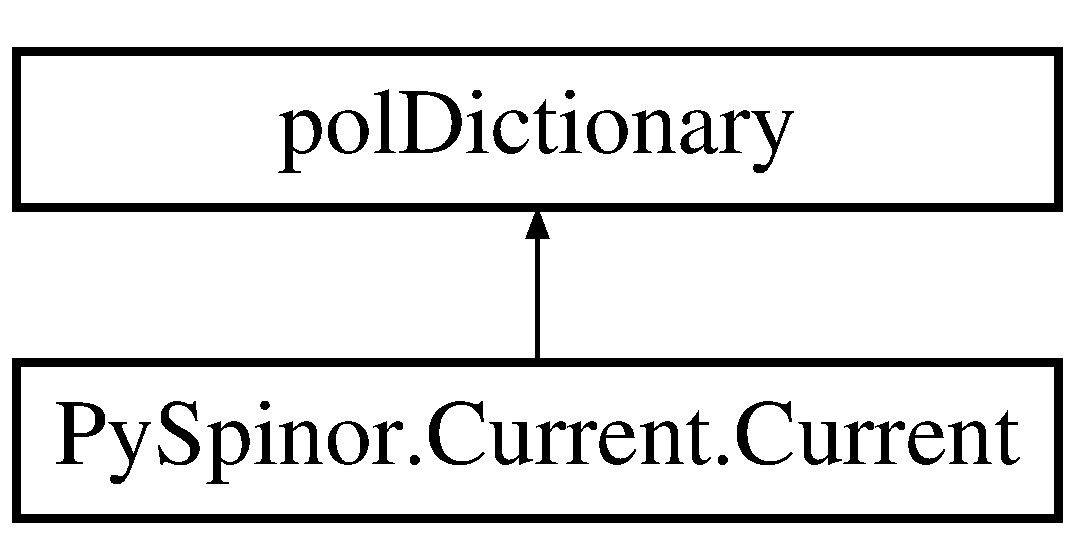
\includegraphics[height=2.000000cm]{class_py_spinor_1_1_current_1_1_current}
\end{center}
\end{figure}
\subsection*{Classes}
\begin{DoxyCompactItemize}
\item 
class \hyperlink{class_py_spinor_1_1_current_1_1_current_1_1current}{current}
\begin{DoxyCompactList}\small\item\em Lorentz vector currents. \end{DoxyCompactList}\end{DoxyCompactItemize}
\subsection*{Public Member Functions}
\begin{DoxyCompactItemize}
\item 
def \hyperlink{class_py_spinor_1_1_current_1_1_current_a5a4c380b36f9757b46a434a4c42ea3ed}{init\+From\+Dict} (cls, instance, Dict)
\item 
def \hyperlink{class_py_spinor_1_1_current_1_1_current_a6f8c8e4850fda84bc354636c2c47f57a}{\+\_\+\+\_\+init\+\_\+\+\_\+}
\begin{DoxyCompactList}\small\item\em \hyperlink{class_py_spinor_1_1_current_1_1_current}{Current} constructor. \end{DoxyCompactList}\item 
def \hyperlink{class_py_spinor_1_1_current_1_1_current_a8d0a4648405116998091d1e1de6a6b58}{\+\_\+\+\_\+rmul\+\_\+\+\_\+} (self, other)
\item 
def \hyperlink{class_py_spinor_1_1_current_1_1_current_ac24728ae3294273b179751ee920df9c8}{\+\_\+\+\_\+div\+\_\+\+\_\+} (self, other)
\end{DoxyCompactItemize}
\subsection*{Public Attributes}
\begin{DoxyCompactItemize}
\item 
\hyperlink{class_py_spinor_1_1_current_1_1_current_af39cbee6c5dffe193c6b741958161abb}{index}
\item 
\hyperlink{class_py_spinor_1_1_current_1_1_current_a1d7c4ad7c95a09c99a5ac532fb667da1}{upper}
\item 
\hyperlink{class_py_spinor_1_1_current_1_1_current_a3e56175e0c447734990b0da3791448df}{spin1}
\item 
\hyperlink{class_py_spinor_1_1_current_1_1_current_afdb9923c8f80cc9031e8874a601f04a9}{spin2}
\item 
\hyperlink{class_py_spinor_1_1_current_1_1_current_a9de458c8ced89ac2051796ea7b737873}{polarisations}
\end{DoxyCompactItemize}


\subsection{Detailed Description}
Class storing spinor current information. 

\subsection{Constructor \& Destructor Documentation}
\hypertarget{class_py_spinor_1_1_current_1_1_current_a6f8c8e4850fda84bc354636c2c47f57a}{}\index{Py\+Spinor\+::\+Current\+::\+Current@{Py\+Spinor\+::\+Current\+::\+Current}!\+\_\+\+\_\+init\+\_\+\+\_\+@{\+\_\+\+\_\+init\+\_\+\+\_\+}}
\index{\+\_\+\+\_\+init\+\_\+\+\_\+@{\+\_\+\+\_\+init\+\_\+\+\_\+}!Py\+Spinor\+::\+Current\+::\+Current@{Py\+Spinor\+::\+Current\+::\+Current}}
\subsubsection[{\+\_\+\+\_\+init\+\_\+\+\_\+}]{\setlength{\rightskip}{0pt plus 5cm}def Py\+Spinor.\+Current.\+Current.\+\_\+\+\_\+init\+\_\+\+\_\+ (
\begin{DoxyParamCaption}
\item[{}]{self, }
\item[{}]{spin1, }
\item[{}]{index, }
\item[{}]{spin2, }
\item[{}]{upper = {\ttfamily True}, }
\item[{}]{Dict = {\ttfamily None}}
\end{DoxyParamCaption}
)}\label{class_py_spinor_1_1_current_1_1_current_a6f8c8e4850fda84bc354636c2c47f57a}


\hyperlink{class_py_spinor_1_1_current_1_1_current}{Current} constructor. 



\subsection{Member Function Documentation}
\hypertarget{class_py_spinor_1_1_current_1_1_current_ac24728ae3294273b179751ee920df9c8}{}\index{Py\+Spinor\+::\+Current\+::\+Current@{Py\+Spinor\+::\+Current\+::\+Current}!\+\_\+\+\_\+div\+\_\+\+\_\+@{\+\_\+\+\_\+div\+\_\+\+\_\+}}
\index{\+\_\+\+\_\+div\+\_\+\+\_\+@{\+\_\+\+\_\+div\+\_\+\+\_\+}!Py\+Spinor\+::\+Current\+::\+Current@{Py\+Spinor\+::\+Current\+::\+Current}}
\subsubsection[{\+\_\+\+\_\+div\+\_\+\+\_\+}]{\setlength{\rightskip}{0pt plus 5cm}def Py\+Spinor.\+Current.\+Current.\+\_\+\+\_\+div\+\_\+\+\_\+ (
\begin{DoxyParamCaption}
\item[{}]{self, }
\item[{}]{other}
\end{DoxyParamCaption}
)}\label{class_py_spinor_1_1_current_1_1_current_ac24728ae3294273b179751ee920df9c8}
\hypertarget{class_py_spinor_1_1_current_1_1_current_a8d0a4648405116998091d1e1de6a6b58}{}\index{Py\+Spinor\+::\+Current\+::\+Current@{Py\+Spinor\+::\+Current\+::\+Current}!\+\_\+\+\_\+rmul\+\_\+\+\_\+@{\+\_\+\+\_\+rmul\+\_\+\+\_\+}}
\index{\+\_\+\+\_\+rmul\+\_\+\+\_\+@{\+\_\+\+\_\+rmul\+\_\+\+\_\+}!Py\+Spinor\+::\+Current\+::\+Current@{Py\+Spinor\+::\+Current\+::\+Current}}
\subsubsection[{\+\_\+\+\_\+rmul\+\_\+\+\_\+}]{\setlength{\rightskip}{0pt plus 5cm}def Py\+Spinor.\+Current.\+Current.\+\_\+\+\_\+rmul\+\_\+\+\_\+ (
\begin{DoxyParamCaption}
\item[{}]{self, }
\item[{}]{other}
\end{DoxyParamCaption}
)}\label{class_py_spinor_1_1_current_1_1_current_a8d0a4648405116998091d1e1de6a6b58}
\hypertarget{class_py_spinor_1_1_current_1_1_current_a5a4c380b36f9757b46a434a4c42ea3ed}{}\index{Py\+Spinor\+::\+Current\+::\+Current@{Py\+Spinor\+::\+Current\+::\+Current}!init\+From\+Dict@{init\+From\+Dict}}
\index{init\+From\+Dict@{init\+From\+Dict}!Py\+Spinor\+::\+Current\+::\+Current@{Py\+Spinor\+::\+Current\+::\+Current}}
\subsubsection[{init\+From\+Dict}]{\setlength{\rightskip}{0pt plus 5cm}def Py\+Spinor.\+Current.\+Current.\+init\+From\+Dict (
\begin{DoxyParamCaption}
\item[{}]{cls, }
\item[{}]{instance, }
\item[{}]{Dict}
\end{DoxyParamCaption}
)}\label{class_py_spinor_1_1_current_1_1_current_a5a4c380b36f9757b46a434a4c42ea3ed}


\subsection{Member Data Documentation}
\hypertarget{class_py_spinor_1_1_current_1_1_current_af39cbee6c5dffe193c6b741958161abb}{}\index{Py\+Spinor\+::\+Current\+::\+Current@{Py\+Spinor\+::\+Current\+::\+Current}!index@{index}}
\index{index@{index}!Py\+Spinor\+::\+Current\+::\+Current@{Py\+Spinor\+::\+Current\+::\+Current}}
\subsubsection[{index}]{\setlength{\rightskip}{0pt plus 5cm}Py\+Spinor.\+Current.\+Current.\+index}\label{class_py_spinor_1_1_current_1_1_current_af39cbee6c5dffe193c6b741958161abb}
\hypertarget{class_py_spinor_1_1_current_1_1_current_a9de458c8ced89ac2051796ea7b737873}{}\index{Py\+Spinor\+::\+Current\+::\+Current@{Py\+Spinor\+::\+Current\+::\+Current}!polarisations@{polarisations}}
\index{polarisations@{polarisations}!Py\+Spinor\+::\+Current\+::\+Current@{Py\+Spinor\+::\+Current\+::\+Current}}
\subsubsection[{polarisations}]{\setlength{\rightskip}{0pt plus 5cm}Py\+Spinor.\+Current.\+Current.\+polarisations}\label{class_py_spinor_1_1_current_1_1_current_a9de458c8ced89ac2051796ea7b737873}
\hypertarget{class_py_spinor_1_1_current_1_1_current_a3e56175e0c447734990b0da3791448df}{}\index{Py\+Spinor\+::\+Current\+::\+Current@{Py\+Spinor\+::\+Current\+::\+Current}!spin1@{spin1}}
\index{spin1@{spin1}!Py\+Spinor\+::\+Current\+::\+Current@{Py\+Spinor\+::\+Current\+::\+Current}}
\subsubsection[{spin1}]{\setlength{\rightskip}{0pt plus 5cm}Py\+Spinor.\+Current.\+Current.\+spin1}\label{class_py_spinor_1_1_current_1_1_current_a3e56175e0c447734990b0da3791448df}
\hypertarget{class_py_spinor_1_1_current_1_1_current_afdb9923c8f80cc9031e8874a601f04a9}{}\index{Py\+Spinor\+::\+Current\+::\+Current@{Py\+Spinor\+::\+Current\+::\+Current}!spin2@{spin2}}
\index{spin2@{spin2}!Py\+Spinor\+::\+Current\+::\+Current@{Py\+Spinor\+::\+Current\+::\+Current}}
\subsubsection[{spin2}]{\setlength{\rightskip}{0pt plus 5cm}Py\+Spinor.\+Current.\+Current.\+spin2}\label{class_py_spinor_1_1_current_1_1_current_afdb9923c8f80cc9031e8874a601f04a9}
\hypertarget{class_py_spinor_1_1_current_1_1_current_a1d7c4ad7c95a09c99a5ac532fb667da1}{}\index{Py\+Spinor\+::\+Current\+::\+Current@{Py\+Spinor\+::\+Current\+::\+Current}!upper@{upper}}
\index{upper@{upper}!Py\+Spinor\+::\+Current\+::\+Current@{Py\+Spinor\+::\+Current\+::\+Current}}
\subsubsection[{upper}]{\setlength{\rightskip}{0pt plus 5cm}Py\+Spinor.\+Current.\+Current.\+upper}\label{class_py_spinor_1_1_current_1_1_current_a1d7c4ad7c95a09c99a5ac532fb667da1}


The documentation for this class was generated from the following file\+:\begin{DoxyCompactItemize}
\item 
Py\+Spinor/\hyperlink{_current_8py}{Current.\+py}\end{DoxyCompactItemize}

\hypertarget{class_py_spinor_1_1_current_1_1_current_1_1current}{}\section{Py\+Spinor.\+Current.\+Current.\+current Class Reference}
\label{class_py_spinor_1_1_current_1_1_current_1_1current}\index{Py\+Spinor.\+Current.\+Current.\+current@{Py\+Spinor.\+Current.\+Current.\+current}}


Lorentz vector currents.  


Inheritance diagram for Py\+Spinor.\+Current.\+Current.\+current\+:\begin{figure}[H]
\begin{center}
\leavevmode
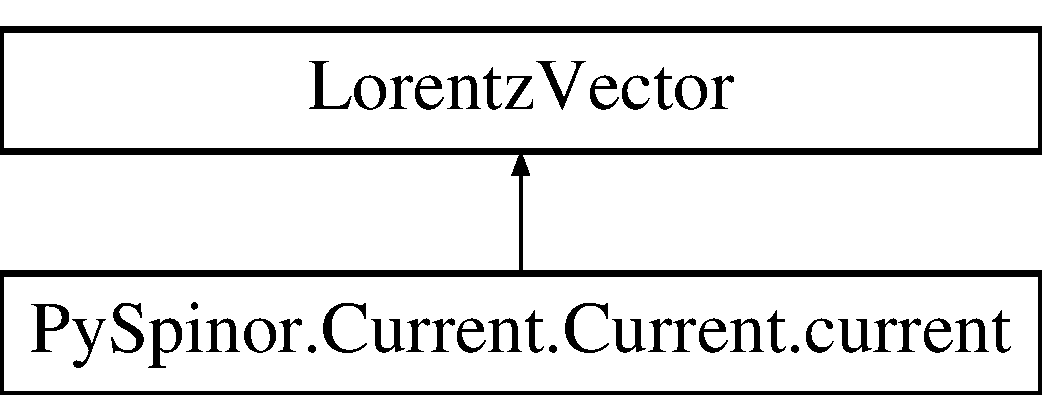
\includegraphics[height=2.000000cm]{class_py_spinor_1_1_current_1_1_current_1_1current}
\end{center}
\end{figure}
\subsection*{Public Member Functions}
\begin{DoxyCompactItemize}
\item 
def \hyperlink{class_py_spinor_1_1_current_1_1_current_1_1current_ae3b366c2162861b95a9e153ea12e7dfa}{\+\_\+\+\_\+init\+\_\+\+\_\+}
\end{DoxyCompactItemize}
\subsection*{Public Attributes}
\begin{DoxyCompactItemize}
\item 
\hyperlink{class_py_spinor_1_1_current_1_1_current_1_1current_afb15d94b551fdbc5f8aeb7bf995202f4}{spin1}
\item 
\hyperlink{class_py_spinor_1_1_current_1_1_current_1_1current_a0bebca6b3a193936ea6f4feb0fca1fb2}{spin2}
\item 
\hyperlink{class_py_spinor_1_1_current_1_1_current_1_1current_a6c01b0e5a656cbd005b1612db36d6abb}{upper}
\item 
\hyperlink{class_py_spinor_1_1_current_1_1_current_1_1current_ab20a21fcc050dc05b3ec49c429a932e6}{index}
\end{DoxyCompactItemize}
\subsection*{Static Public Attributes}
\begin{DoxyCompactItemize}
\item 
dictionary \hyperlink{class_py_spinor_1_1_current_1_1_current_1_1current_a0e70234795fa01a35b0ce9da4862daf9}{indices} = \{\}
\end{DoxyCompactItemize}


\subsection{Detailed Description}
Lorentz vector currents. 

\subsection{Constructor \& Destructor Documentation}
\hypertarget{class_py_spinor_1_1_current_1_1_current_1_1current_ae3b366c2162861b95a9e153ea12e7dfa}{}\index{Py\+Spinor\+::\+Current\+::\+Current\+::current@{Py\+Spinor\+::\+Current\+::\+Current\+::current}!\+\_\+\+\_\+init\+\_\+\+\_\+@{\+\_\+\+\_\+init\+\_\+\+\_\+}}
\index{\+\_\+\+\_\+init\+\_\+\+\_\+@{\+\_\+\+\_\+init\+\_\+\+\_\+}!Py\+Spinor\+::\+Current\+::\+Current\+::current@{Py\+Spinor\+::\+Current\+::\+Current\+::current}}
\subsubsection[{\+\_\+\+\_\+init\+\_\+\+\_\+}]{\setlength{\rightskip}{0pt plus 5cm}def Py\+Spinor.\+Current.\+Current.\+current.\+\_\+\+\_\+init\+\_\+\+\_\+ (
\begin{DoxyParamCaption}
\item[{}]{self, }
\item[{}]{spin1, }
\item[{}]{index, }
\item[{}]{spin2, }
\item[{}]{upper = {\ttfamily True}, }
\item[{}]{Vector = {\ttfamily None}}
\end{DoxyParamCaption}
)}\label{class_py_spinor_1_1_current_1_1_current_1_1current_ae3b366c2162861b95a9e153ea12e7dfa}


\subsection{Member Data Documentation}
\hypertarget{class_py_spinor_1_1_current_1_1_current_1_1current_ab20a21fcc050dc05b3ec49c429a932e6}{}\index{Py\+Spinor\+::\+Current\+::\+Current\+::current@{Py\+Spinor\+::\+Current\+::\+Current\+::current}!index@{index}}
\index{index@{index}!Py\+Spinor\+::\+Current\+::\+Current\+::current@{Py\+Spinor\+::\+Current\+::\+Current\+::current}}
\subsubsection[{index}]{\setlength{\rightskip}{0pt plus 5cm}Py\+Spinor.\+Current.\+Current.\+current.\+index}\label{class_py_spinor_1_1_current_1_1_current_1_1current_ab20a21fcc050dc05b3ec49c429a932e6}
\hypertarget{class_py_spinor_1_1_current_1_1_current_1_1current_a0e70234795fa01a35b0ce9da4862daf9}{}\index{Py\+Spinor\+::\+Current\+::\+Current\+::current@{Py\+Spinor\+::\+Current\+::\+Current\+::current}!indices@{indices}}
\index{indices@{indices}!Py\+Spinor\+::\+Current\+::\+Current\+::current@{Py\+Spinor\+::\+Current\+::\+Current\+::current}}
\subsubsection[{indices}]{\setlength{\rightskip}{0pt plus 5cm}dictionary Py\+Spinor.\+Current.\+Current.\+current.\+indices = \{\}\hspace{0.3cm}{\ttfamily [static]}}\label{class_py_spinor_1_1_current_1_1_current_1_1current_a0e70234795fa01a35b0ce9da4862daf9}
\hypertarget{class_py_spinor_1_1_current_1_1_current_1_1current_afb15d94b551fdbc5f8aeb7bf995202f4}{}\index{Py\+Spinor\+::\+Current\+::\+Current\+::current@{Py\+Spinor\+::\+Current\+::\+Current\+::current}!spin1@{spin1}}
\index{spin1@{spin1}!Py\+Spinor\+::\+Current\+::\+Current\+::current@{Py\+Spinor\+::\+Current\+::\+Current\+::current}}
\subsubsection[{spin1}]{\setlength{\rightskip}{0pt plus 5cm}Py\+Spinor.\+Current.\+Current.\+current.\+spin1}\label{class_py_spinor_1_1_current_1_1_current_1_1current_afb15d94b551fdbc5f8aeb7bf995202f4}
\hypertarget{class_py_spinor_1_1_current_1_1_current_1_1current_a0bebca6b3a193936ea6f4feb0fca1fb2}{}\index{Py\+Spinor\+::\+Current\+::\+Current\+::current@{Py\+Spinor\+::\+Current\+::\+Current\+::current}!spin2@{spin2}}
\index{spin2@{spin2}!Py\+Spinor\+::\+Current\+::\+Current\+::current@{Py\+Spinor\+::\+Current\+::\+Current\+::current}}
\subsubsection[{spin2}]{\setlength{\rightskip}{0pt plus 5cm}Py\+Spinor.\+Current.\+Current.\+current.\+spin2}\label{class_py_spinor_1_1_current_1_1_current_1_1current_a0bebca6b3a193936ea6f4feb0fca1fb2}
\hypertarget{class_py_spinor_1_1_current_1_1_current_1_1current_a6c01b0e5a656cbd005b1612db36d6abb}{}\index{Py\+Spinor\+::\+Current\+::\+Current\+::current@{Py\+Spinor\+::\+Current\+::\+Current\+::current}!upper@{upper}}
\index{upper@{upper}!Py\+Spinor\+::\+Current\+::\+Current\+::current@{Py\+Spinor\+::\+Current\+::\+Current\+::current}}
\subsubsection[{upper}]{\setlength{\rightskip}{0pt plus 5cm}Py\+Spinor.\+Current.\+Current.\+current.\+upper}\label{class_py_spinor_1_1_current_1_1_current_1_1current_a6c01b0e5a656cbd005b1612db36d6abb}


The documentation for this class was generated from the following file\+:\begin{DoxyCompactItemize}
\item 
Py\+Spinor/\hyperlink{_current_8py}{Current.\+py}\end{DoxyCompactItemize}

\hypertarget{class_py_spinor_1_1_gluon_1_1_gluon}{}\section{Py\+Spinor.\+Gluon.\+Gluon Class Reference}
\label{class_py_spinor_1_1_gluon_1_1_gluon}\index{Py\+Spinor.\+Gluon.\+Gluon@{Py\+Spinor.\+Gluon.\+Gluon}}


\hyperlink{class_py_spinor_1_1_gluon_1_1_gluon}{Gluon} class.  


Inheritance diagram for Py\+Spinor.\+Gluon.\+Gluon\+:\begin{figure}[H]
\begin{center}
\leavevmode
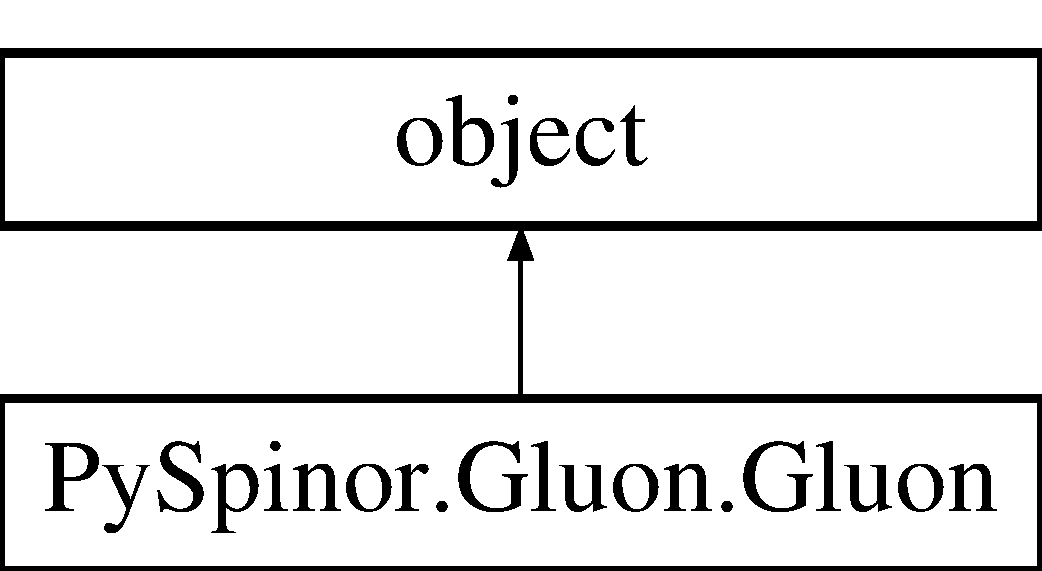
\includegraphics[height=2.000000cm]{class_py_spinor_1_1_gluon_1_1_gluon}
\end{center}
\end{figure}
\subsection*{Public Member Functions}
\begin{DoxyCompactItemize}
\item 
def \hyperlink{class_py_spinor_1_1_gluon_1_1_gluon_a57608c7c1b5c7d7bc10f3924059686be}{\+\_\+\+\_\+init\+\_\+\+\_\+}
\item 
def \hyperlink{class_py_spinor_1_1_gluon_1_1_gluon_aeee21fbdf614f791756ec5bfc25aec7c}{\+\_\+\+\_\+str\+\_\+\+\_\+} (self)
\item 
def \hyperlink{class_py_spinor_1_1_gluon_1_1_gluon_a89302eeb19dc10b7fb1ffe2a1affc678}{\+\_\+\+\_\+getitem\+\_\+\+\_\+} (self, pol)
\end{DoxyCompactItemize}
\subsection*{Public Attributes}
\begin{DoxyCompactItemize}
\item 
\hyperlink{class_py_spinor_1_1_gluon_1_1_gluon_ab6e6d38292b6b8e63ed888df78fa23ff}{p}
\item 
\hyperlink{class_py_spinor_1_1_gluon_1_1_gluon_a4cc0aee09287cfb077f59e2c6665145d}{r}
\item 
\hyperlink{class_py_spinor_1_1_gluon_1_1_gluon_a890f8133ad0546d319f9319789def113}{index}
\item 
\hyperlink{class_py_spinor_1_1_gluon_1_1_gluon_afc4fcbb98438d15efdfea2df9702c6ac}{upper}
\item 
\hyperlink{class_py_spinor_1_1_gluon_1_1_gluon_aa77d6b321ed6a1cb5dbf72bd1f6645f0}{vector}
\end{DoxyCompactItemize}


\subsection{Detailed Description}
\hyperlink{class_py_spinor_1_1_gluon_1_1_gluon}{Gluon} class. 

\subsection{Constructor \& Destructor Documentation}
\hypertarget{class_py_spinor_1_1_gluon_1_1_gluon_a57608c7c1b5c7d7bc10f3924059686be}{}\index{Py\+Spinor\+::\+Gluon\+::\+Gluon@{Py\+Spinor\+::\+Gluon\+::\+Gluon}!\+\_\+\+\_\+init\+\_\+\+\_\+@{\+\_\+\+\_\+init\+\_\+\+\_\+}}
\index{\+\_\+\+\_\+init\+\_\+\+\_\+@{\+\_\+\+\_\+init\+\_\+\+\_\+}!Py\+Spinor\+::\+Gluon\+::\+Gluon@{Py\+Spinor\+::\+Gluon\+::\+Gluon}}
\subsubsection[{\+\_\+\+\_\+init\+\_\+\+\_\+}]{\setlength{\rightskip}{0pt plus 5cm}def Py\+Spinor.\+Gluon.\+Gluon.\+\_\+\+\_\+init\+\_\+\+\_\+ (
\begin{DoxyParamCaption}
\item[{}]{self, }
\item[{}]{p, }
\item[{}]{r, }
\item[{}]{index, }
\item[{}]{upper = {\ttfamily True}}
\end{DoxyParamCaption}
)}\label{class_py_spinor_1_1_gluon_1_1_gluon_a57608c7c1b5c7d7bc10f3924059686be}


\subsection{Member Function Documentation}
\hypertarget{class_py_spinor_1_1_gluon_1_1_gluon_a89302eeb19dc10b7fb1ffe2a1affc678}{}\index{Py\+Spinor\+::\+Gluon\+::\+Gluon@{Py\+Spinor\+::\+Gluon\+::\+Gluon}!\+\_\+\+\_\+getitem\+\_\+\+\_\+@{\+\_\+\+\_\+getitem\+\_\+\+\_\+}}
\index{\+\_\+\+\_\+getitem\+\_\+\+\_\+@{\+\_\+\+\_\+getitem\+\_\+\+\_\+}!Py\+Spinor\+::\+Gluon\+::\+Gluon@{Py\+Spinor\+::\+Gluon\+::\+Gluon}}
\subsubsection[{\+\_\+\+\_\+getitem\+\_\+\+\_\+}]{\setlength{\rightskip}{0pt plus 5cm}def Py\+Spinor.\+Gluon.\+Gluon.\+\_\+\+\_\+getitem\+\_\+\+\_\+ (
\begin{DoxyParamCaption}
\item[{}]{self, }
\item[{}]{pol}
\end{DoxyParamCaption}
)}\label{class_py_spinor_1_1_gluon_1_1_gluon_a89302eeb19dc10b7fb1ffe2a1affc678}
\hypertarget{class_py_spinor_1_1_gluon_1_1_gluon_aeee21fbdf614f791756ec5bfc25aec7c}{}\index{Py\+Spinor\+::\+Gluon\+::\+Gluon@{Py\+Spinor\+::\+Gluon\+::\+Gluon}!\+\_\+\+\_\+str\+\_\+\+\_\+@{\+\_\+\+\_\+str\+\_\+\+\_\+}}
\index{\+\_\+\+\_\+str\+\_\+\+\_\+@{\+\_\+\+\_\+str\+\_\+\+\_\+}!Py\+Spinor\+::\+Gluon\+::\+Gluon@{Py\+Spinor\+::\+Gluon\+::\+Gluon}}
\subsubsection[{\+\_\+\+\_\+str\+\_\+\+\_\+}]{\setlength{\rightskip}{0pt plus 5cm}def Py\+Spinor.\+Gluon.\+Gluon.\+\_\+\+\_\+str\+\_\+\+\_\+ (
\begin{DoxyParamCaption}
\item[{}]{self}
\end{DoxyParamCaption}
)}\label{class_py_spinor_1_1_gluon_1_1_gluon_aeee21fbdf614f791756ec5bfc25aec7c}


\subsection{Member Data Documentation}
\hypertarget{class_py_spinor_1_1_gluon_1_1_gluon_a890f8133ad0546d319f9319789def113}{}\index{Py\+Spinor\+::\+Gluon\+::\+Gluon@{Py\+Spinor\+::\+Gluon\+::\+Gluon}!index@{index}}
\index{index@{index}!Py\+Spinor\+::\+Gluon\+::\+Gluon@{Py\+Spinor\+::\+Gluon\+::\+Gluon}}
\subsubsection[{index}]{\setlength{\rightskip}{0pt plus 5cm}Py\+Spinor.\+Gluon.\+Gluon.\+index}\label{class_py_spinor_1_1_gluon_1_1_gluon_a890f8133ad0546d319f9319789def113}
\hypertarget{class_py_spinor_1_1_gluon_1_1_gluon_ab6e6d38292b6b8e63ed888df78fa23ff}{}\index{Py\+Spinor\+::\+Gluon\+::\+Gluon@{Py\+Spinor\+::\+Gluon\+::\+Gluon}!p@{p}}
\index{p@{p}!Py\+Spinor\+::\+Gluon\+::\+Gluon@{Py\+Spinor\+::\+Gluon\+::\+Gluon}}
\subsubsection[{p}]{\setlength{\rightskip}{0pt plus 5cm}Py\+Spinor.\+Gluon.\+Gluon.\+p}\label{class_py_spinor_1_1_gluon_1_1_gluon_ab6e6d38292b6b8e63ed888df78fa23ff}
\hypertarget{class_py_spinor_1_1_gluon_1_1_gluon_a4cc0aee09287cfb077f59e2c6665145d}{}\index{Py\+Spinor\+::\+Gluon\+::\+Gluon@{Py\+Spinor\+::\+Gluon\+::\+Gluon}!r@{r}}
\index{r@{r}!Py\+Spinor\+::\+Gluon\+::\+Gluon@{Py\+Spinor\+::\+Gluon\+::\+Gluon}}
\subsubsection[{r}]{\setlength{\rightskip}{0pt plus 5cm}Py\+Spinor.\+Gluon.\+Gluon.\+r}\label{class_py_spinor_1_1_gluon_1_1_gluon_a4cc0aee09287cfb077f59e2c6665145d}
\hypertarget{class_py_spinor_1_1_gluon_1_1_gluon_afc4fcbb98438d15efdfea2df9702c6ac}{}\index{Py\+Spinor\+::\+Gluon\+::\+Gluon@{Py\+Spinor\+::\+Gluon\+::\+Gluon}!upper@{upper}}
\index{upper@{upper}!Py\+Spinor\+::\+Gluon\+::\+Gluon@{Py\+Spinor\+::\+Gluon\+::\+Gluon}}
\subsubsection[{upper}]{\setlength{\rightskip}{0pt plus 5cm}Py\+Spinor.\+Gluon.\+Gluon.\+upper}\label{class_py_spinor_1_1_gluon_1_1_gluon_afc4fcbb98438d15efdfea2df9702c6ac}
\hypertarget{class_py_spinor_1_1_gluon_1_1_gluon_aa77d6b321ed6a1cb5dbf72bd1f6645f0}{}\index{Py\+Spinor\+::\+Gluon\+::\+Gluon@{Py\+Spinor\+::\+Gluon\+::\+Gluon}!vector@{vector}}
\index{vector@{vector}!Py\+Spinor\+::\+Gluon\+::\+Gluon@{Py\+Spinor\+::\+Gluon\+::\+Gluon}}
\subsubsection[{vector}]{\setlength{\rightskip}{0pt plus 5cm}Py\+Spinor.\+Gluon.\+Gluon.\+vector}\label{class_py_spinor_1_1_gluon_1_1_gluon_aa77d6b321ed6a1cb5dbf72bd1f6645f0}


The documentation for this class was generated from the following file\+:\begin{DoxyCompactItemize}
\item 
Py\+Spinor/\hyperlink{_gluon_8py}{Gluon.\+py}\end{DoxyCompactItemize}

\hypertarget{class_py_spinor_1_1_lorentz_vector_1_1_lorentz_vector}{}\section{Py\+Spinor.\+Lorentz\+Vector.\+Lorentz\+Vector Class Reference}
\label{class_py_spinor_1_1_lorentz_vector_1_1_lorentz_vector}\index{Py\+Spinor.\+Lorentz\+Vector.\+Lorentz\+Vector@{Py\+Spinor.\+Lorentz\+Vector.\+Lorentz\+Vector}}


Parent class for anything with a Lorentz index Will require full rewrite inheriting from new \hyperlink{namespace_py_spinor_1_1_tensor}{Tensor} class and likely with Lorentz\+Index class to be written.  


Inheritance diagram for Py\+Spinor.\+Lorentz\+Vector.\+Lorentz\+Vector\+:\begin{figure}[H]
\begin{center}
\leavevmode
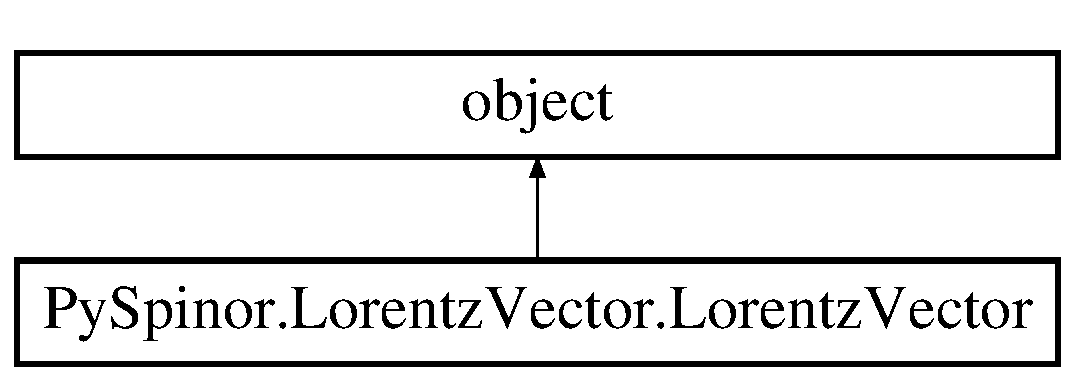
\includegraphics[height=2.000000cm]{class_py_spinor_1_1_lorentz_vector_1_1_lorentz_vector}
\end{center}
\end{figure}
\subsection*{Public Member Functions}
\begin{DoxyCompactItemize}
\item 
def \hyperlink{class_py_spinor_1_1_lorentz_vector_1_1_lorentz_vector_aae8d47664e6e334ffc3765e081f77c4f}{\+\_\+\+\_\+init\+\_\+\+\_\+}
\item 
def \hyperlink{class_py_spinor_1_1_lorentz_vector_1_1_lorentz_vector_a8adef627e38fbef234c90de0378bdf40}{T}
\item 
def \hyperlink{class_py_spinor_1_1_lorentz_vector_1_1_lorentz_vector_abb4ed2b7f72ceea64756d9e27ef59e3a}{X}
\item 
def \hyperlink{class_py_spinor_1_1_lorentz_vector_1_1_lorentz_vector_ac2449f2d40ae954dc7be2e3ab335ad18}{Y}
\item 
def \hyperlink{class_py_spinor_1_1_lorentz_vector_1_1_lorentz_vector_ad05ad87908b5c645af2ae67cbf5ea269}{Z}
\item 
def \hyperlink{class_py_spinor_1_1_lorentz_vector_1_1_lorentz_vector_a89043007a937453bbc9adc76fa4d3276}{conjugate} (self)
\item 
def \hyperlink{class_py_spinor_1_1_lorentz_vector_1_1_lorentz_vector_a83544cd8c242999f7be5cfc29e61e31c}{\+\_\+\+\_\+call\+\_\+\+\_\+} (self, \hyperlink{class_py_spinor_1_1_lorentz_vector_1_1_lorentz_vector_a11da34cf107e38100b3bfb509eac2d1f}{index})
\begin{DoxyCompactList}\small\item\em Allows vector to be called with specific index name given by string argument. \end{DoxyCompactList}\item 
def \hyperlink{class_py_spinor_1_1_lorentz_vector_1_1_lorentz_vector_af7e9f0d16494f38a0c8aab1290e73b51}{\+\_\+\+\_\+str\+\_\+\+\_\+} (self)
\item 
def \hyperlink{class_py_spinor_1_1_lorentz_vector_1_1_lorentz_vector_ab127e64670ad904cd9fc85afdf78cd79}{\+\_\+\+\_\+sub\+\_\+\+\_\+} (self, other)
\begin{DoxyCompactList}\small\item\em Subtraction for co-\/ and contra-\/variant vectors (resp) \end{DoxyCompactList}\item 
def \hyperlink{class_py_spinor_1_1_lorentz_vector_1_1_lorentz_vector_aa0925be56ef69c512eb861129b37fcb0}{\+\_\+\+\_\+add\+\_\+\+\_\+} (self, other)
\begin{DoxyCompactList}\small\item\em Addition for co-\/ and contra-\/variant vectors (resp) \end{DoxyCompactList}\item 
def \hyperlink{class_py_spinor_1_1_lorentz_vector_1_1_lorentz_vector_af7178d2be820ce5c50e01c8c03fb3cef}{\+\_\+\+\_\+neg\+\_\+\+\_\+} (self)
\begin{DoxyCompactList}\small\item\em Negation of vector elements. \end{DoxyCompactList}\item 
def \hyperlink{class_py_spinor_1_1_lorentz_vector_1_1_lorentz_vector_a4b6ca093f716869de228bd9611e8cd40}{\+\_\+\+\_\+mul\+\_\+\+\_\+} (self, other)
\begin{DoxyCompactList}\small\item\em Defines vector-\/scalar and vector-\/matrix multiplication (numpy matrix input required for latter) \end{DoxyCompactList}\item 
def \hyperlink{class_py_spinor_1_1_lorentz_vector_1_1_lorentz_vector_a9c2aeb0c1d496ffd0d6fe4e3d551f451}{\+\_\+\+\_\+pow\+\_\+\+\_\+} (self, exponent)
\begin{DoxyCompactList}\small\item\em Allows for powers of vectors through the vector self inner product. \end{DoxyCompactList}\item 
def \hyperlink{class_py_spinor_1_1_lorentz_vector_1_1_lorentz_vector_a1affc9d1cf09f3f7dbe85742c7ce7a6c}{\+\_\+\+\_\+getitem\+\_\+\+\_\+} (self, \hyperlink{class_py_spinor_1_1_lorentz_vector_1_1_lorentz_vector_a11da34cf107e38100b3bfb509eac2d1f}{index})
\begin{DoxyCompactList}\small\item\em Returns particular element of vector specified by numerical index. \end{DoxyCompactList}\item 
def \hyperlink{class_py_spinor_1_1_lorentz_vector_1_1_lorentz_vector_a8c669764e80ef2c4100a898e9b1ab7d6}{\+\_\+\+\_\+rmul\+\_\+\+\_\+} (self, other)
\begin{DoxyCompactList}\small\item\em Scalar-\/vector and matrix-\/vector multiplication. \end{DoxyCompactList}\item 
def \hyperlink{class_py_spinor_1_1_lorentz_vector_1_1_lorentz_vector_a8fbfe5ece750a1a53a99f609972ad616}{\+\_\+\+\_\+eq\+\_\+\+\_\+} (self, other)
\begin{DoxyCompactList}\small\item\em Comparison of float elements of a vector up to some degree of tolerance T\+O\+L\+E\+R\+A\+N\+C\+E defined in \hyperlink{_common_8py}{Common.\+py}. \end{DoxyCompactList}\item 
def \hyperlink{class_py_spinor_1_1_lorentz_vector_1_1_lorentz_vector_ad011c74a579e139893eb6705b9b70af1}{dot} (self, other)
\begin{DoxyCompactList}\small\item\em Dot product for two four vectors. \end{DoxyCompactList}\item 
def \hyperlink{class_py_spinor_1_1_lorentz_vector_1_1_lorentz_vector_a9ce48fd10a5b006f9a42423d689c7e38}{slashed} (self)
\begin{DoxyCompactList}\small\item\em Feynman slash notation. \end{DoxyCompactList}\item 
def \hyperlink{class_py_spinor_1_1_lorentz_vector_1_1_lorentz_vector_af7c7e87a6ca9cd879f5f17edd1e474af}{\+\_\+\+\_\+div\+\_\+\+\_\+} (self, other)
\begin{DoxyCompactList}\small\item\em Division by scalar. \end{DoxyCompactList}\item 
def \hyperlink{class_py_spinor_1_1_lorentz_vector_1_1_lorentz_vector_a1a40b84d71110ea6280f0d53a371e8ff}{Lower} (self)
\begin{DoxyCompactList}\small\item\em Lower index. \end{DoxyCompactList}\item 
def \hyperlink{class_py_spinor_1_1_lorentz_vector_1_1_lorentz_vector_a2de4017ffc816aeed0ebf7e8dd189464}{Raise} (self)
\begin{DoxyCompactList}\small\item\em Raise index. \end{DoxyCompactList}\item 
def \hyperlink{class_py_spinor_1_1_lorentz_vector_1_1_lorentz_vector_ab8854208c107ed5ef4fec5d3036e0220}{co} (self)
\begin{DoxyCompactList}\small\item\em Bool\+: Is the \hyperlink{class_py_spinor_1_1_lorentz_vector_1_1_lorentz_vector}{Lorentz\+Vector} covariant? \end{DoxyCompactList}\item 
def \hyperlink{class_py_spinor_1_1_lorentz_vector_1_1_lorentz_vector_ab2fcc827cfd71331e8f62e9c6bf95197}{contra} (self)
\begin{DoxyCompactList}\small\item\em Bool\+: Is the \hyperlink{class_py_spinor_1_1_lorentz_vector_1_1_lorentz_vector}{Lorentz\+Vector} contravariant? \end{DoxyCompactList}\item 
def \hyperlink{class_py_spinor_1_1_lorentz_vector_1_1_lorentz_vector_acf1bb09347d6e573c95e8e4c1c9d99c6}{set\+Vector} (self, \hyperlink{class_py_spinor_1_1_lorentz_vector_1_1_lorentz_vector_a094448bd25db3631dfda6402c7c258e1}{vector})
\begin{DoxyCompactList}\small\item\em Sets elements given 1-\/d numpy array. \end{DoxyCompactList}\item 
def \hyperlink{class_py_spinor_1_1_lorentz_vector_1_1_lorentz_vector_aa37cd941a7f2cbd8369f0a5e28925576}{print\+Index} (self)
\begin{DoxyCompactList}\small\item\em Print the index for this current. \end{DoxyCompactList}\item 
def \hyperlink{class_py_spinor_1_1_lorentz_vector_1_1_lorentz_vector_ae739123740bfd3809dd9b885afad90eb}{set\+Index} (self, \hyperlink{class_py_spinor_1_1_lorentz_vector_1_1_lorentz_vector_a11da34cf107e38100b3bfb509eac2d1f}{index})
\begin{DoxyCompactList}\small\item\em Change the index for an instance. \end{DoxyCompactList}\item 
def \hyperlink{class_py_spinor_1_1_lorentz_vector_1_1_lorentz_vector_a5a7c97faead7b3e7f08885b4ebb1f24d}{boost} (\hyperlink{class_py_spinor_1_1_lorentz_vector_1_1_lorentz_vector_a094448bd25db3631dfda6402c7c258e1}{vector}, b\+X, b\+Y, b\+Z)
\begin{DoxyCompactList}\small\item\em Perform a Lorentz boost. \end{DoxyCompactList}\end{DoxyCompactItemize}
\subsection*{Public Attributes}
\begin{DoxyCompactItemize}
\item 
\hyperlink{class_py_spinor_1_1_lorentz_vector_1_1_lorentz_vector_ad789506f2bd56ab54bb743d84092aa77}{upper}
\item 
\hyperlink{class_py_spinor_1_1_lorentz_vector_1_1_lorentz_vector_a11da34cf107e38100b3bfb509eac2d1f}{index}
\item 
\hyperlink{class_py_spinor_1_1_lorentz_vector_1_1_lorentz_vector_a094448bd25db3631dfda6402c7c258e1}{vector}
\end{DoxyCompactItemize}


\subsection{Detailed Description}
Parent class for anything with a Lorentz index Will require full rewrite inheriting from new \hyperlink{namespace_py_spinor_1_1_tensor}{Tensor} class and likely with Lorentz\+Index class to be written. 

\subsection{Constructor \& Destructor Documentation}
\hypertarget{class_py_spinor_1_1_lorentz_vector_1_1_lorentz_vector_aae8d47664e6e334ffc3765e081f77c4f}{}\index{Py\+Spinor\+::\+Lorentz\+Vector\+::\+Lorentz\+Vector@{Py\+Spinor\+::\+Lorentz\+Vector\+::\+Lorentz\+Vector}!\+\_\+\+\_\+init\+\_\+\+\_\+@{\+\_\+\+\_\+init\+\_\+\+\_\+}}
\index{\+\_\+\+\_\+init\+\_\+\+\_\+@{\+\_\+\+\_\+init\+\_\+\+\_\+}!Py\+Spinor\+::\+Lorentz\+Vector\+::\+Lorentz\+Vector@{Py\+Spinor\+::\+Lorentz\+Vector\+::\+Lorentz\+Vector}}
\subsubsection[{\+\_\+\+\_\+init\+\_\+\+\_\+}]{\setlength{\rightskip}{0pt plus 5cm}def Py\+Spinor.\+Lorentz\+Vector.\+Lorentz\+Vector.\+\_\+\+\_\+init\+\_\+\+\_\+ (
\begin{DoxyParamCaption}
\item[{}]{self, }
\item[{}]{E, }
\item[{}]{X, }
\item[{}]{Y, }
\item[{}]{Z, }
\item[{}]{upper, }
\item[{}]{index = {\ttfamily \textquotesingle{}mu\textquotesingle{}}}
\end{DoxyParamCaption}
)}\label{class_py_spinor_1_1_lorentz_vector_1_1_lorentz_vector_aae8d47664e6e334ffc3765e081f77c4f}


\subsection{Member Function Documentation}
\hypertarget{class_py_spinor_1_1_lorentz_vector_1_1_lorentz_vector_aa0925be56ef69c512eb861129b37fcb0}{}\index{Py\+Spinor\+::\+Lorentz\+Vector\+::\+Lorentz\+Vector@{Py\+Spinor\+::\+Lorentz\+Vector\+::\+Lorentz\+Vector}!\+\_\+\+\_\+add\+\_\+\+\_\+@{\+\_\+\+\_\+add\+\_\+\+\_\+}}
\index{\+\_\+\+\_\+add\+\_\+\+\_\+@{\+\_\+\+\_\+add\+\_\+\+\_\+}!Py\+Spinor\+::\+Lorentz\+Vector\+::\+Lorentz\+Vector@{Py\+Spinor\+::\+Lorentz\+Vector\+::\+Lorentz\+Vector}}
\subsubsection[{\+\_\+\+\_\+add\+\_\+\+\_\+}]{\setlength{\rightskip}{0pt plus 5cm}def Py\+Spinor.\+Lorentz\+Vector.\+Lorentz\+Vector.\+\_\+\+\_\+add\+\_\+\+\_\+ (
\begin{DoxyParamCaption}
\item[{}]{self, }
\item[{}]{other}
\end{DoxyParamCaption}
)}\label{class_py_spinor_1_1_lorentz_vector_1_1_lorentz_vector_aa0925be56ef69c512eb861129b37fcb0}


Addition for co-\/ and contra-\/variant vectors (resp) 

\hypertarget{class_py_spinor_1_1_lorentz_vector_1_1_lorentz_vector_a83544cd8c242999f7be5cfc29e61e31c}{}\index{Py\+Spinor\+::\+Lorentz\+Vector\+::\+Lorentz\+Vector@{Py\+Spinor\+::\+Lorentz\+Vector\+::\+Lorentz\+Vector}!\+\_\+\+\_\+call\+\_\+\+\_\+@{\+\_\+\+\_\+call\+\_\+\+\_\+}}
\index{\+\_\+\+\_\+call\+\_\+\+\_\+@{\+\_\+\+\_\+call\+\_\+\+\_\+}!Py\+Spinor\+::\+Lorentz\+Vector\+::\+Lorentz\+Vector@{Py\+Spinor\+::\+Lorentz\+Vector\+::\+Lorentz\+Vector}}
\subsubsection[{\+\_\+\+\_\+call\+\_\+\+\_\+}]{\setlength{\rightskip}{0pt plus 5cm}def Py\+Spinor.\+Lorentz\+Vector.\+Lorentz\+Vector.\+\_\+\+\_\+call\+\_\+\+\_\+ (
\begin{DoxyParamCaption}
\item[{}]{self, }
\item[{}]{index}
\end{DoxyParamCaption}
)}\label{class_py_spinor_1_1_lorentz_vector_1_1_lorentz_vector_a83544cd8c242999f7be5cfc29e61e31c}


Allows vector to be called with specific index name given by string argument. 

\hypertarget{class_py_spinor_1_1_lorentz_vector_1_1_lorentz_vector_af7c7e87a6ca9cd879f5f17edd1e474af}{}\index{Py\+Spinor\+::\+Lorentz\+Vector\+::\+Lorentz\+Vector@{Py\+Spinor\+::\+Lorentz\+Vector\+::\+Lorentz\+Vector}!\+\_\+\+\_\+div\+\_\+\+\_\+@{\+\_\+\+\_\+div\+\_\+\+\_\+}}
\index{\+\_\+\+\_\+div\+\_\+\+\_\+@{\+\_\+\+\_\+div\+\_\+\+\_\+}!Py\+Spinor\+::\+Lorentz\+Vector\+::\+Lorentz\+Vector@{Py\+Spinor\+::\+Lorentz\+Vector\+::\+Lorentz\+Vector}}
\subsubsection[{\+\_\+\+\_\+div\+\_\+\+\_\+}]{\setlength{\rightskip}{0pt plus 5cm}def Py\+Spinor.\+Lorentz\+Vector.\+Lorentz\+Vector.\+\_\+\+\_\+div\+\_\+\+\_\+ (
\begin{DoxyParamCaption}
\item[{}]{self, }
\item[{}]{other}
\end{DoxyParamCaption}
)}\label{class_py_spinor_1_1_lorentz_vector_1_1_lorentz_vector_af7c7e87a6ca9cd879f5f17edd1e474af}


Division by scalar. 

\hypertarget{class_py_spinor_1_1_lorentz_vector_1_1_lorentz_vector_a8fbfe5ece750a1a53a99f609972ad616}{}\index{Py\+Spinor\+::\+Lorentz\+Vector\+::\+Lorentz\+Vector@{Py\+Spinor\+::\+Lorentz\+Vector\+::\+Lorentz\+Vector}!\+\_\+\+\_\+eq\+\_\+\+\_\+@{\+\_\+\+\_\+eq\+\_\+\+\_\+}}
\index{\+\_\+\+\_\+eq\+\_\+\+\_\+@{\+\_\+\+\_\+eq\+\_\+\+\_\+}!Py\+Spinor\+::\+Lorentz\+Vector\+::\+Lorentz\+Vector@{Py\+Spinor\+::\+Lorentz\+Vector\+::\+Lorentz\+Vector}}
\subsubsection[{\+\_\+\+\_\+eq\+\_\+\+\_\+}]{\setlength{\rightskip}{0pt plus 5cm}def Py\+Spinor.\+Lorentz\+Vector.\+Lorentz\+Vector.\+\_\+\+\_\+eq\+\_\+\+\_\+ (
\begin{DoxyParamCaption}
\item[{}]{self, }
\item[{}]{other}
\end{DoxyParamCaption}
)}\label{class_py_spinor_1_1_lorentz_vector_1_1_lorentz_vector_a8fbfe5ece750a1a53a99f609972ad616}


Comparison of float elements of a vector up to some degree of tolerance T\+O\+L\+E\+R\+A\+N\+C\+E defined in \hyperlink{_common_8py}{Common.\+py}. 

\hypertarget{class_py_spinor_1_1_lorentz_vector_1_1_lorentz_vector_a1affc9d1cf09f3f7dbe85742c7ce7a6c}{}\index{Py\+Spinor\+::\+Lorentz\+Vector\+::\+Lorentz\+Vector@{Py\+Spinor\+::\+Lorentz\+Vector\+::\+Lorentz\+Vector}!\+\_\+\+\_\+getitem\+\_\+\+\_\+@{\+\_\+\+\_\+getitem\+\_\+\+\_\+}}
\index{\+\_\+\+\_\+getitem\+\_\+\+\_\+@{\+\_\+\+\_\+getitem\+\_\+\+\_\+}!Py\+Spinor\+::\+Lorentz\+Vector\+::\+Lorentz\+Vector@{Py\+Spinor\+::\+Lorentz\+Vector\+::\+Lorentz\+Vector}}
\subsubsection[{\+\_\+\+\_\+getitem\+\_\+\+\_\+}]{\setlength{\rightskip}{0pt plus 5cm}def Py\+Spinor.\+Lorentz\+Vector.\+Lorentz\+Vector.\+\_\+\+\_\+getitem\+\_\+\+\_\+ (
\begin{DoxyParamCaption}
\item[{}]{self, }
\item[{}]{index}
\end{DoxyParamCaption}
)}\label{class_py_spinor_1_1_lorentz_vector_1_1_lorentz_vector_a1affc9d1cf09f3f7dbe85742c7ce7a6c}


Returns particular element of vector specified by numerical index. 

\hypertarget{class_py_spinor_1_1_lorentz_vector_1_1_lorentz_vector_a4b6ca093f716869de228bd9611e8cd40}{}\index{Py\+Spinor\+::\+Lorentz\+Vector\+::\+Lorentz\+Vector@{Py\+Spinor\+::\+Lorentz\+Vector\+::\+Lorentz\+Vector}!\+\_\+\+\_\+mul\+\_\+\+\_\+@{\+\_\+\+\_\+mul\+\_\+\+\_\+}}
\index{\+\_\+\+\_\+mul\+\_\+\+\_\+@{\+\_\+\+\_\+mul\+\_\+\+\_\+}!Py\+Spinor\+::\+Lorentz\+Vector\+::\+Lorentz\+Vector@{Py\+Spinor\+::\+Lorentz\+Vector\+::\+Lorentz\+Vector}}
\subsubsection[{\+\_\+\+\_\+mul\+\_\+\+\_\+}]{\setlength{\rightskip}{0pt plus 5cm}def Py\+Spinor.\+Lorentz\+Vector.\+Lorentz\+Vector.\+\_\+\+\_\+mul\+\_\+\+\_\+ (
\begin{DoxyParamCaption}
\item[{}]{self, }
\item[{}]{other}
\end{DoxyParamCaption}
)}\label{class_py_spinor_1_1_lorentz_vector_1_1_lorentz_vector_a4b6ca093f716869de228bd9611e8cd40}


Defines vector-\/scalar and vector-\/matrix multiplication (numpy matrix input required for latter) 

\hypertarget{class_py_spinor_1_1_lorentz_vector_1_1_lorentz_vector_af7178d2be820ce5c50e01c8c03fb3cef}{}\index{Py\+Spinor\+::\+Lorentz\+Vector\+::\+Lorentz\+Vector@{Py\+Spinor\+::\+Lorentz\+Vector\+::\+Lorentz\+Vector}!\+\_\+\+\_\+neg\+\_\+\+\_\+@{\+\_\+\+\_\+neg\+\_\+\+\_\+}}
\index{\+\_\+\+\_\+neg\+\_\+\+\_\+@{\+\_\+\+\_\+neg\+\_\+\+\_\+}!Py\+Spinor\+::\+Lorentz\+Vector\+::\+Lorentz\+Vector@{Py\+Spinor\+::\+Lorentz\+Vector\+::\+Lorentz\+Vector}}
\subsubsection[{\+\_\+\+\_\+neg\+\_\+\+\_\+}]{\setlength{\rightskip}{0pt plus 5cm}def Py\+Spinor.\+Lorentz\+Vector.\+Lorentz\+Vector.\+\_\+\+\_\+neg\+\_\+\+\_\+ (
\begin{DoxyParamCaption}
\item[{}]{self}
\end{DoxyParamCaption}
)}\label{class_py_spinor_1_1_lorentz_vector_1_1_lorentz_vector_af7178d2be820ce5c50e01c8c03fb3cef}


Negation of vector elements. 

\hypertarget{class_py_spinor_1_1_lorentz_vector_1_1_lorentz_vector_a9c2aeb0c1d496ffd0d6fe4e3d551f451}{}\index{Py\+Spinor\+::\+Lorentz\+Vector\+::\+Lorentz\+Vector@{Py\+Spinor\+::\+Lorentz\+Vector\+::\+Lorentz\+Vector}!\+\_\+\+\_\+pow\+\_\+\+\_\+@{\+\_\+\+\_\+pow\+\_\+\+\_\+}}
\index{\+\_\+\+\_\+pow\+\_\+\+\_\+@{\+\_\+\+\_\+pow\+\_\+\+\_\+}!Py\+Spinor\+::\+Lorentz\+Vector\+::\+Lorentz\+Vector@{Py\+Spinor\+::\+Lorentz\+Vector\+::\+Lorentz\+Vector}}
\subsubsection[{\+\_\+\+\_\+pow\+\_\+\+\_\+}]{\setlength{\rightskip}{0pt plus 5cm}def Py\+Spinor.\+Lorentz\+Vector.\+Lorentz\+Vector.\+\_\+\+\_\+pow\+\_\+\+\_\+ (
\begin{DoxyParamCaption}
\item[{}]{self, }
\item[{}]{exponent}
\end{DoxyParamCaption}
)}\label{class_py_spinor_1_1_lorentz_vector_1_1_lorentz_vector_a9c2aeb0c1d496ffd0d6fe4e3d551f451}


Allows for powers of vectors through the vector self inner product. 

\hypertarget{class_py_spinor_1_1_lorentz_vector_1_1_lorentz_vector_a8c669764e80ef2c4100a898e9b1ab7d6}{}\index{Py\+Spinor\+::\+Lorentz\+Vector\+::\+Lorentz\+Vector@{Py\+Spinor\+::\+Lorentz\+Vector\+::\+Lorentz\+Vector}!\+\_\+\+\_\+rmul\+\_\+\+\_\+@{\+\_\+\+\_\+rmul\+\_\+\+\_\+}}
\index{\+\_\+\+\_\+rmul\+\_\+\+\_\+@{\+\_\+\+\_\+rmul\+\_\+\+\_\+}!Py\+Spinor\+::\+Lorentz\+Vector\+::\+Lorentz\+Vector@{Py\+Spinor\+::\+Lorentz\+Vector\+::\+Lorentz\+Vector}}
\subsubsection[{\+\_\+\+\_\+rmul\+\_\+\+\_\+}]{\setlength{\rightskip}{0pt plus 5cm}def Py\+Spinor.\+Lorentz\+Vector.\+Lorentz\+Vector.\+\_\+\+\_\+rmul\+\_\+\+\_\+ (
\begin{DoxyParamCaption}
\item[{}]{self, }
\item[{}]{other}
\end{DoxyParamCaption}
)}\label{class_py_spinor_1_1_lorentz_vector_1_1_lorentz_vector_a8c669764e80ef2c4100a898e9b1ab7d6}


Scalar-\/vector and matrix-\/vector multiplication. 

\hypertarget{class_py_spinor_1_1_lorentz_vector_1_1_lorentz_vector_af7e9f0d16494f38a0c8aab1290e73b51}{}\index{Py\+Spinor\+::\+Lorentz\+Vector\+::\+Lorentz\+Vector@{Py\+Spinor\+::\+Lorentz\+Vector\+::\+Lorentz\+Vector}!\+\_\+\+\_\+str\+\_\+\+\_\+@{\+\_\+\+\_\+str\+\_\+\+\_\+}}
\index{\+\_\+\+\_\+str\+\_\+\+\_\+@{\+\_\+\+\_\+str\+\_\+\+\_\+}!Py\+Spinor\+::\+Lorentz\+Vector\+::\+Lorentz\+Vector@{Py\+Spinor\+::\+Lorentz\+Vector\+::\+Lorentz\+Vector}}
\subsubsection[{\+\_\+\+\_\+str\+\_\+\+\_\+}]{\setlength{\rightskip}{0pt plus 5cm}def Py\+Spinor.\+Lorentz\+Vector.\+Lorentz\+Vector.\+\_\+\+\_\+str\+\_\+\+\_\+ (
\begin{DoxyParamCaption}
\item[{}]{self}
\end{DoxyParamCaption}
)}\label{class_py_spinor_1_1_lorentz_vector_1_1_lorentz_vector_af7e9f0d16494f38a0c8aab1290e73b51}
\hypertarget{class_py_spinor_1_1_lorentz_vector_1_1_lorentz_vector_ab127e64670ad904cd9fc85afdf78cd79}{}\index{Py\+Spinor\+::\+Lorentz\+Vector\+::\+Lorentz\+Vector@{Py\+Spinor\+::\+Lorentz\+Vector\+::\+Lorentz\+Vector}!\+\_\+\+\_\+sub\+\_\+\+\_\+@{\+\_\+\+\_\+sub\+\_\+\+\_\+}}
\index{\+\_\+\+\_\+sub\+\_\+\+\_\+@{\+\_\+\+\_\+sub\+\_\+\+\_\+}!Py\+Spinor\+::\+Lorentz\+Vector\+::\+Lorentz\+Vector@{Py\+Spinor\+::\+Lorentz\+Vector\+::\+Lorentz\+Vector}}
\subsubsection[{\+\_\+\+\_\+sub\+\_\+\+\_\+}]{\setlength{\rightskip}{0pt plus 5cm}def Py\+Spinor.\+Lorentz\+Vector.\+Lorentz\+Vector.\+\_\+\+\_\+sub\+\_\+\+\_\+ (
\begin{DoxyParamCaption}
\item[{}]{self, }
\item[{}]{other}
\end{DoxyParamCaption}
)}\label{class_py_spinor_1_1_lorentz_vector_1_1_lorentz_vector_ab127e64670ad904cd9fc85afdf78cd79}


Subtraction for co-\/ and contra-\/variant vectors (resp) 

\hypertarget{class_py_spinor_1_1_lorentz_vector_1_1_lorentz_vector_a5a7c97faead7b3e7f08885b4ebb1f24d}{}\index{Py\+Spinor\+::\+Lorentz\+Vector\+::\+Lorentz\+Vector@{Py\+Spinor\+::\+Lorentz\+Vector\+::\+Lorentz\+Vector}!boost@{boost}}
\index{boost@{boost}!Py\+Spinor\+::\+Lorentz\+Vector\+::\+Lorentz\+Vector@{Py\+Spinor\+::\+Lorentz\+Vector\+::\+Lorentz\+Vector}}
\subsubsection[{boost}]{\setlength{\rightskip}{0pt plus 5cm}def Py\+Spinor.\+Lorentz\+Vector.\+Lorentz\+Vector.\+boost (
\begin{DoxyParamCaption}
\item[{}]{vector, }
\item[{}]{b\+X, }
\item[{}]{b\+Y, }
\item[{}]{b\+Z}
\end{DoxyParamCaption}
)}\label{class_py_spinor_1_1_lorentz_vector_1_1_lorentz_vector_a5a7c97faead7b3e7f08885b4ebb1f24d}


Perform a Lorentz boost. 

\hypertarget{class_py_spinor_1_1_lorentz_vector_1_1_lorentz_vector_ab8854208c107ed5ef4fec5d3036e0220}{}\index{Py\+Spinor\+::\+Lorentz\+Vector\+::\+Lorentz\+Vector@{Py\+Spinor\+::\+Lorentz\+Vector\+::\+Lorentz\+Vector}!co@{co}}
\index{co@{co}!Py\+Spinor\+::\+Lorentz\+Vector\+::\+Lorentz\+Vector@{Py\+Spinor\+::\+Lorentz\+Vector\+::\+Lorentz\+Vector}}
\subsubsection[{co}]{\setlength{\rightskip}{0pt plus 5cm}def Py\+Spinor.\+Lorentz\+Vector.\+Lorentz\+Vector.\+co (
\begin{DoxyParamCaption}
\item[{}]{self}
\end{DoxyParamCaption}
)}\label{class_py_spinor_1_1_lorentz_vector_1_1_lorentz_vector_ab8854208c107ed5ef4fec5d3036e0220}


Bool\+: Is the \hyperlink{class_py_spinor_1_1_lorentz_vector_1_1_lorentz_vector}{Lorentz\+Vector} covariant? 

\hypertarget{class_py_spinor_1_1_lorentz_vector_1_1_lorentz_vector_a89043007a937453bbc9adc76fa4d3276}{}\index{Py\+Spinor\+::\+Lorentz\+Vector\+::\+Lorentz\+Vector@{Py\+Spinor\+::\+Lorentz\+Vector\+::\+Lorentz\+Vector}!conjugate@{conjugate}}
\index{conjugate@{conjugate}!Py\+Spinor\+::\+Lorentz\+Vector\+::\+Lorentz\+Vector@{Py\+Spinor\+::\+Lorentz\+Vector\+::\+Lorentz\+Vector}}
\subsubsection[{conjugate}]{\setlength{\rightskip}{0pt plus 5cm}def Py\+Spinor.\+Lorentz\+Vector.\+Lorentz\+Vector.\+conjugate (
\begin{DoxyParamCaption}
\item[{}]{self}
\end{DoxyParamCaption}
)}\label{class_py_spinor_1_1_lorentz_vector_1_1_lorentz_vector_a89043007a937453bbc9adc76fa4d3276}
\hypertarget{class_py_spinor_1_1_lorentz_vector_1_1_lorentz_vector_ab2fcc827cfd71331e8f62e9c6bf95197}{}\index{Py\+Spinor\+::\+Lorentz\+Vector\+::\+Lorentz\+Vector@{Py\+Spinor\+::\+Lorentz\+Vector\+::\+Lorentz\+Vector}!contra@{contra}}
\index{contra@{contra}!Py\+Spinor\+::\+Lorentz\+Vector\+::\+Lorentz\+Vector@{Py\+Spinor\+::\+Lorentz\+Vector\+::\+Lorentz\+Vector}}
\subsubsection[{contra}]{\setlength{\rightskip}{0pt plus 5cm}def Py\+Spinor.\+Lorentz\+Vector.\+Lorentz\+Vector.\+contra (
\begin{DoxyParamCaption}
\item[{}]{self}
\end{DoxyParamCaption}
)}\label{class_py_spinor_1_1_lorentz_vector_1_1_lorentz_vector_ab2fcc827cfd71331e8f62e9c6bf95197}


Bool\+: Is the \hyperlink{class_py_spinor_1_1_lorentz_vector_1_1_lorentz_vector}{Lorentz\+Vector} contravariant? 

\hypertarget{class_py_spinor_1_1_lorentz_vector_1_1_lorentz_vector_ad011c74a579e139893eb6705b9b70af1}{}\index{Py\+Spinor\+::\+Lorentz\+Vector\+::\+Lorentz\+Vector@{Py\+Spinor\+::\+Lorentz\+Vector\+::\+Lorentz\+Vector}!dot@{dot}}
\index{dot@{dot}!Py\+Spinor\+::\+Lorentz\+Vector\+::\+Lorentz\+Vector@{Py\+Spinor\+::\+Lorentz\+Vector\+::\+Lorentz\+Vector}}
\subsubsection[{dot}]{\setlength{\rightskip}{0pt plus 5cm}def Py\+Spinor.\+Lorentz\+Vector.\+Lorentz\+Vector.\+dot (
\begin{DoxyParamCaption}
\item[{}]{self, }
\item[{}]{other}
\end{DoxyParamCaption}
)}\label{class_py_spinor_1_1_lorentz_vector_1_1_lorentz_vector_ad011c74a579e139893eb6705b9b70af1}


Dot product for two four vectors. 

\hypertarget{class_py_spinor_1_1_lorentz_vector_1_1_lorentz_vector_a1a40b84d71110ea6280f0d53a371e8ff}{}\index{Py\+Spinor\+::\+Lorentz\+Vector\+::\+Lorentz\+Vector@{Py\+Spinor\+::\+Lorentz\+Vector\+::\+Lorentz\+Vector}!Lower@{Lower}}
\index{Lower@{Lower}!Py\+Spinor\+::\+Lorentz\+Vector\+::\+Lorentz\+Vector@{Py\+Spinor\+::\+Lorentz\+Vector\+::\+Lorentz\+Vector}}
\subsubsection[{Lower}]{\setlength{\rightskip}{0pt plus 5cm}def Py\+Spinor.\+Lorentz\+Vector.\+Lorentz\+Vector.\+Lower (
\begin{DoxyParamCaption}
\item[{}]{self}
\end{DoxyParamCaption}
)}\label{class_py_spinor_1_1_lorentz_vector_1_1_lorentz_vector_a1a40b84d71110ea6280f0d53a371e8ff}


Lower index. 

\hypertarget{class_py_spinor_1_1_lorentz_vector_1_1_lorentz_vector_aa37cd941a7f2cbd8369f0a5e28925576}{}\index{Py\+Spinor\+::\+Lorentz\+Vector\+::\+Lorentz\+Vector@{Py\+Spinor\+::\+Lorentz\+Vector\+::\+Lorentz\+Vector}!print\+Index@{print\+Index}}
\index{print\+Index@{print\+Index}!Py\+Spinor\+::\+Lorentz\+Vector\+::\+Lorentz\+Vector@{Py\+Spinor\+::\+Lorentz\+Vector\+::\+Lorentz\+Vector}}
\subsubsection[{print\+Index}]{\setlength{\rightskip}{0pt plus 5cm}def Py\+Spinor.\+Lorentz\+Vector.\+Lorentz\+Vector.\+print\+Index (
\begin{DoxyParamCaption}
\item[{}]{self}
\end{DoxyParamCaption}
)}\label{class_py_spinor_1_1_lorentz_vector_1_1_lorentz_vector_aa37cd941a7f2cbd8369f0a5e28925576}


Print the index for this current. 

\hypertarget{class_py_spinor_1_1_lorentz_vector_1_1_lorentz_vector_a2de4017ffc816aeed0ebf7e8dd189464}{}\index{Py\+Spinor\+::\+Lorentz\+Vector\+::\+Lorentz\+Vector@{Py\+Spinor\+::\+Lorentz\+Vector\+::\+Lorentz\+Vector}!Raise@{Raise}}
\index{Raise@{Raise}!Py\+Spinor\+::\+Lorentz\+Vector\+::\+Lorentz\+Vector@{Py\+Spinor\+::\+Lorentz\+Vector\+::\+Lorentz\+Vector}}
\subsubsection[{Raise}]{\setlength{\rightskip}{0pt plus 5cm}def Py\+Spinor.\+Lorentz\+Vector.\+Lorentz\+Vector.\+Raise (
\begin{DoxyParamCaption}
\item[{}]{self}
\end{DoxyParamCaption}
)}\label{class_py_spinor_1_1_lorentz_vector_1_1_lorentz_vector_a2de4017ffc816aeed0ebf7e8dd189464}


Raise index. 

\hypertarget{class_py_spinor_1_1_lorentz_vector_1_1_lorentz_vector_ae739123740bfd3809dd9b885afad90eb}{}\index{Py\+Spinor\+::\+Lorentz\+Vector\+::\+Lorentz\+Vector@{Py\+Spinor\+::\+Lorentz\+Vector\+::\+Lorentz\+Vector}!set\+Index@{set\+Index}}
\index{set\+Index@{set\+Index}!Py\+Spinor\+::\+Lorentz\+Vector\+::\+Lorentz\+Vector@{Py\+Spinor\+::\+Lorentz\+Vector\+::\+Lorentz\+Vector}}
\subsubsection[{set\+Index}]{\setlength{\rightskip}{0pt plus 5cm}def Py\+Spinor.\+Lorentz\+Vector.\+Lorentz\+Vector.\+set\+Index (
\begin{DoxyParamCaption}
\item[{}]{self, }
\item[{}]{index}
\end{DoxyParamCaption}
)}\label{class_py_spinor_1_1_lorentz_vector_1_1_lorentz_vector_ae739123740bfd3809dd9b885afad90eb}


Change the index for an instance. 

\hypertarget{class_py_spinor_1_1_lorentz_vector_1_1_lorentz_vector_acf1bb09347d6e573c95e8e4c1c9d99c6}{}\index{Py\+Spinor\+::\+Lorentz\+Vector\+::\+Lorentz\+Vector@{Py\+Spinor\+::\+Lorentz\+Vector\+::\+Lorentz\+Vector}!set\+Vector@{set\+Vector}}
\index{set\+Vector@{set\+Vector}!Py\+Spinor\+::\+Lorentz\+Vector\+::\+Lorentz\+Vector@{Py\+Spinor\+::\+Lorentz\+Vector\+::\+Lorentz\+Vector}}
\subsubsection[{set\+Vector}]{\setlength{\rightskip}{0pt plus 5cm}def Py\+Spinor.\+Lorentz\+Vector.\+Lorentz\+Vector.\+set\+Vector (
\begin{DoxyParamCaption}
\item[{}]{self, }
\item[{}]{vector}
\end{DoxyParamCaption}
)}\label{class_py_spinor_1_1_lorentz_vector_1_1_lorentz_vector_acf1bb09347d6e573c95e8e4c1c9d99c6}


Sets elements given 1-\/d numpy array. 

\hypertarget{class_py_spinor_1_1_lorentz_vector_1_1_lorentz_vector_a9ce48fd10a5b006f9a42423d689c7e38}{}\index{Py\+Spinor\+::\+Lorentz\+Vector\+::\+Lorentz\+Vector@{Py\+Spinor\+::\+Lorentz\+Vector\+::\+Lorentz\+Vector}!slashed@{slashed}}
\index{slashed@{slashed}!Py\+Spinor\+::\+Lorentz\+Vector\+::\+Lorentz\+Vector@{Py\+Spinor\+::\+Lorentz\+Vector\+::\+Lorentz\+Vector}}
\subsubsection[{slashed}]{\setlength{\rightskip}{0pt plus 5cm}def Py\+Spinor.\+Lorentz\+Vector.\+Lorentz\+Vector.\+slashed (
\begin{DoxyParamCaption}
\item[{}]{self}
\end{DoxyParamCaption}
)}\label{class_py_spinor_1_1_lorentz_vector_1_1_lorentz_vector_a9ce48fd10a5b006f9a42423d689c7e38}


Feynman slash notation. 

\hypertarget{class_py_spinor_1_1_lorentz_vector_1_1_lorentz_vector_a8adef627e38fbef234c90de0378bdf40}{}\index{Py\+Spinor\+::\+Lorentz\+Vector\+::\+Lorentz\+Vector@{Py\+Spinor\+::\+Lorentz\+Vector\+::\+Lorentz\+Vector}!T@{T}}
\index{T@{T}!Py\+Spinor\+::\+Lorentz\+Vector\+::\+Lorentz\+Vector@{Py\+Spinor\+::\+Lorentz\+Vector\+::\+Lorentz\+Vector}}
\subsubsection[{T}]{\setlength{\rightskip}{0pt plus 5cm}def Py\+Spinor.\+Lorentz\+Vector.\+Lorentz\+Vector.\+T (
\begin{DoxyParamCaption}
\item[{}]{self, }
\item[{}]{value = {\ttfamily None}}
\end{DoxyParamCaption}
)}\label{class_py_spinor_1_1_lorentz_vector_1_1_lorentz_vector_a8adef627e38fbef234c90de0378bdf40}
\hypertarget{class_py_spinor_1_1_lorentz_vector_1_1_lorentz_vector_abb4ed2b7f72ceea64756d9e27ef59e3a}{}\index{Py\+Spinor\+::\+Lorentz\+Vector\+::\+Lorentz\+Vector@{Py\+Spinor\+::\+Lorentz\+Vector\+::\+Lorentz\+Vector}!X@{X}}
\index{X@{X}!Py\+Spinor\+::\+Lorentz\+Vector\+::\+Lorentz\+Vector@{Py\+Spinor\+::\+Lorentz\+Vector\+::\+Lorentz\+Vector}}
\subsubsection[{X}]{\setlength{\rightskip}{0pt plus 5cm}def Py\+Spinor.\+Lorentz\+Vector.\+Lorentz\+Vector.\+X (
\begin{DoxyParamCaption}
\item[{}]{self, }
\item[{}]{value = {\ttfamily None}}
\end{DoxyParamCaption}
)}\label{class_py_spinor_1_1_lorentz_vector_1_1_lorentz_vector_abb4ed2b7f72ceea64756d9e27ef59e3a}
\hypertarget{class_py_spinor_1_1_lorentz_vector_1_1_lorentz_vector_ac2449f2d40ae954dc7be2e3ab335ad18}{}\index{Py\+Spinor\+::\+Lorentz\+Vector\+::\+Lorentz\+Vector@{Py\+Spinor\+::\+Lorentz\+Vector\+::\+Lorentz\+Vector}!Y@{Y}}
\index{Y@{Y}!Py\+Spinor\+::\+Lorentz\+Vector\+::\+Lorentz\+Vector@{Py\+Spinor\+::\+Lorentz\+Vector\+::\+Lorentz\+Vector}}
\subsubsection[{Y}]{\setlength{\rightskip}{0pt plus 5cm}def Py\+Spinor.\+Lorentz\+Vector.\+Lorentz\+Vector.\+Y (
\begin{DoxyParamCaption}
\item[{}]{self, }
\item[{}]{value = {\ttfamily None}}
\end{DoxyParamCaption}
)}\label{class_py_spinor_1_1_lorentz_vector_1_1_lorentz_vector_ac2449f2d40ae954dc7be2e3ab335ad18}
\hypertarget{class_py_spinor_1_1_lorentz_vector_1_1_lorentz_vector_ad05ad87908b5c645af2ae67cbf5ea269}{}\index{Py\+Spinor\+::\+Lorentz\+Vector\+::\+Lorentz\+Vector@{Py\+Spinor\+::\+Lorentz\+Vector\+::\+Lorentz\+Vector}!Z@{Z}}
\index{Z@{Z}!Py\+Spinor\+::\+Lorentz\+Vector\+::\+Lorentz\+Vector@{Py\+Spinor\+::\+Lorentz\+Vector\+::\+Lorentz\+Vector}}
\subsubsection[{Z}]{\setlength{\rightskip}{0pt plus 5cm}def Py\+Spinor.\+Lorentz\+Vector.\+Lorentz\+Vector.\+Z (
\begin{DoxyParamCaption}
\item[{}]{self, }
\item[{}]{value = {\ttfamily None}}
\end{DoxyParamCaption}
)}\label{class_py_spinor_1_1_lorentz_vector_1_1_lorentz_vector_ad05ad87908b5c645af2ae67cbf5ea269}


\subsection{Member Data Documentation}
\hypertarget{class_py_spinor_1_1_lorentz_vector_1_1_lorentz_vector_a11da34cf107e38100b3bfb509eac2d1f}{}\index{Py\+Spinor\+::\+Lorentz\+Vector\+::\+Lorentz\+Vector@{Py\+Spinor\+::\+Lorentz\+Vector\+::\+Lorentz\+Vector}!index@{index}}
\index{index@{index}!Py\+Spinor\+::\+Lorentz\+Vector\+::\+Lorentz\+Vector@{Py\+Spinor\+::\+Lorentz\+Vector\+::\+Lorentz\+Vector}}
\subsubsection[{index}]{\setlength{\rightskip}{0pt plus 5cm}Py\+Spinor.\+Lorentz\+Vector.\+Lorentz\+Vector.\+index}\label{class_py_spinor_1_1_lorentz_vector_1_1_lorentz_vector_a11da34cf107e38100b3bfb509eac2d1f}
\hypertarget{class_py_spinor_1_1_lorentz_vector_1_1_lorentz_vector_ad789506f2bd56ab54bb743d84092aa77}{}\index{Py\+Spinor\+::\+Lorentz\+Vector\+::\+Lorentz\+Vector@{Py\+Spinor\+::\+Lorentz\+Vector\+::\+Lorentz\+Vector}!upper@{upper}}
\index{upper@{upper}!Py\+Spinor\+::\+Lorentz\+Vector\+::\+Lorentz\+Vector@{Py\+Spinor\+::\+Lorentz\+Vector\+::\+Lorentz\+Vector}}
\subsubsection[{upper}]{\setlength{\rightskip}{0pt plus 5cm}Py\+Spinor.\+Lorentz\+Vector.\+Lorentz\+Vector.\+upper}\label{class_py_spinor_1_1_lorentz_vector_1_1_lorentz_vector_ad789506f2bd56ab54bb743d84092aa77}
\hypertarget{class_py_spinor_1_1_lorentz_vector_1_1_lorentz_vector_a094448bd25db3631dfda6402c7c258e1}{}\index{Py\+Spinor\+::\+Lorentz\+Vector\+::\+Lorentz\+Vector@{Py\+Spinor\+::\+Lorentz\+Vector\+::\+Lorentz\+Vector}!vector@{vector}}
\index{vector@{vector}!Py\+Spinor\+::\+Lorentz\+Vector\+::\+Lorentz\+Vector@{Py\+Spinor\+::\+Lorentz\+Vector\+::\+Lorentz\+Vector}}
\subsubsection[{vector}]{\setlength{\rightskip}{0pt plus 5cm}Py\+Spinor.\+Lorentz\+Vector.\+Lorentz\+Vector.\+vector}\label{class_py_spinor_1_1_lorentz_vector_1_1_lorentz_vector_a094448bd25db3631dfda6402c7c258e1}


The documentation for this class was generated from the following file\+:\begin{DoxyCompactItemize}
\item 
Py\+Spinor/\hyperlink{_lorentz_vector_8py}{Lorentz\+Vector.\+py}\end{DoxyCompactItemize}

\hypertarget{class_py_spinor_1_1_momenta_1_1_momenta}{}\section{Py\+Spinor.\+Momenta.\+Momenta Class Reference}
\label{class_py_spinor_1_1_momenta_1_1_momenta}\index{Py\+Spinor.\+Momenta.\+Momenta@{Py\+Spinor.\+Momenta.\+Momenta}}


Derived class for particle momenta.  


Inheritance diagram for Py\+Spinor.\+Momenta.\+Momenta\+:\begin{figure}[H]
\begin{center}
\leavevmode
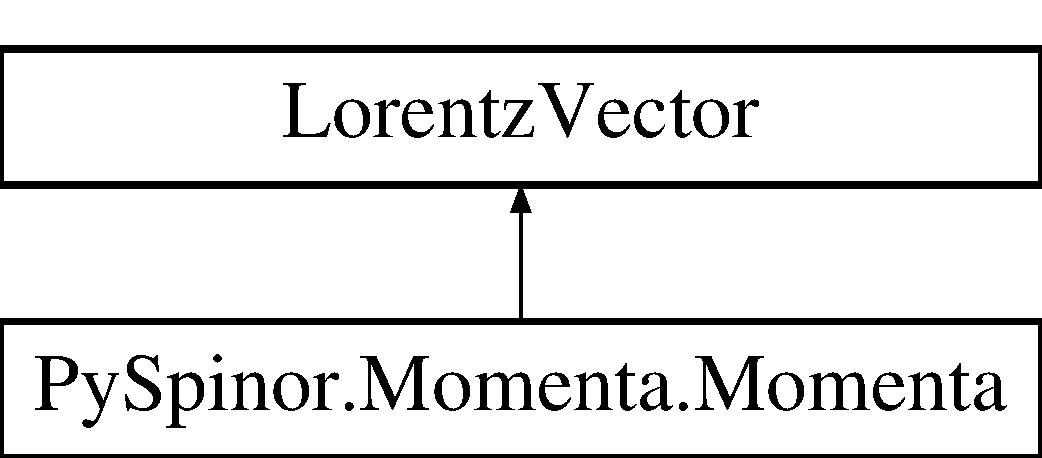
\includegraphics[height=2.000000cm]{class_py_spinor_1_1_momenta_1_1_momenta}
\end{center}
\end{figure}
\subsection*{Public Member Functions}
\begin{DoxyCompactItemize}
\item 
def \hyperlink{class_py_spinor_1_1_momenta_1_1_momenta_a58f6631f07a77727193b8cd3040869b2}{\+\_\+\+\_\+init\+\_\+\+\_\+}
\item 
def \hyperlink{class_py_spinor_1_1_momenta_1_1_momenta_a52d0a5b0986124edaa369b82bfc793b4}{Conserved} (cls)
\item 
def \hyperlink{class_py_spinor_1_1_momenta_1_1_momenta_a7540ed7b06c619de35e7727517f07d47}{is\+Incoming} (self)
\begin{DoxyCompactList}\small\item\em Bool\+: Is the momentum incoming? \end{DoxyCompactList}\item 
def \hyperlink{class_py_spinor_1_1_momenta_1_1_momenta_a670123d7eed72133654307b9b36c5daa}{mass} (self)
\begin{DoxyCompactList}\small\item\em  \+Determine mass from vector squared. \end{DoxyCompactList}\item 
def \hyperlink{class_py_spinor_1_1_momenta_1_1_momenta_ac2eb2567e99f8d68adaafc358672e2e2}{mass2} (self)
\begin{DoxyCompactList}\small\item\em Determing mass squared Why do this though the sqrt of the inner prod? \end{DoxyCompactList}\item 
def \hyperlink{class_py_spinor_1_1_momenta_1_1_momenta_a3710564fb7b6ea3054884395e316ca36}{is\+Massless} (self)
\begin{DoxyCompactList}\small\item\em Bool\+: Is the momentum null? \end{DoxyCompactList}\item 
def \hyperlink{class_py_spinor_1_1_momenta_1_1_momenta_af43d67ac68750a1bf9489886fd5882ca}{plus} (self)
\begin{DoxyCompactList}\small\item\em Lightcone coord plus component. \end{DoxyCompactList}\item 
def \hyperlink{class_py_spinor_1_1_momenta_1_1_momenta_ac812f3fb38392ef3ec74a24513f0afe0}{minus} (self)
\begin{DoxyCompactList}\small\item\em Lightcone coord minus component. \end{DoxyCompactList}\item 
def \hyperlink{class_py_spinor_1_1_momenta_1_1_momenta_a8c2b3a331198822100b2c40e2c3bfafe}{perp} (self)
\begin{DoxyCompactList}\small\item\em Lightcone coord perpendicular components. \end{DoxyCompactList}\item 
def \hyperlink{class_py_spinor_1_1_momenta_1_1_momenta_a8d9de08e70234df6af0d5f52ec793ec8}{boost} (vector, b\+X, b\+Y, b\+Z)
\begin{DoxyCompactList}\small\item\em Lorentz boost momentum. \end{DoxyCompactList}\item 
def \hyperlink{class_py_spinor_1_1_momenta_1_1_momenta_a9c45e296964970075bff55375f5fa083}{decompose} (self)
\begin{DoxyCompactList}\small\item\em Decompost onto special basis. \end{DoxyCompactList}\item 
def \hyperlink{class_py_spinor_1_1_momenta_1_1_momenta_aeb69846d3abfbdc89c2b00edee57d1bf}{\+\_\+\+\_\+add\+\_\+\+\_\+} (self, other)
\item 
def \hyperlink{class_py_spinor_1_1_momenta_1_1_momenta_a6216736ecda0d13749b256cf7c5e1063}{\+\_\+\+\_\+sub\+\_\+\+\_\+} (self, other)
\item 
def \hyperlink{class_py_spinor_1_1_momenta_1_1_momenta_ab2e817c69a9fcd21e926b8bee794c522}{\+\_\+\+\_\+mul\+\_\+\+\_\+} (self, other)
\item 
def \hyperlink{class_py_spinor_1_1_momenta_1_1_momenta_a60fdd62c88311ad0fe38db1972d69433}{\+\_\+\+\_\+rmul\+\_\+\+\_\+} (self, other)
\item 
def \hyperlink{class_py_spinor_1_1_momenta_1_1_momenta_a90d55b09d7dee4e246bc8068a292659c}{\+\_\+\+\_\+div\+\_\+\+\_\+} (self, other)
\end{DoxyCompactItemize}
\subsection*{Public Attributes}
\begin{DoxyCompactItemize}
\item 
\hyperlink{class_py_spinor_1_1_momenta_1_1_momenta_a47a027268693ec412866afb5ec99c6ac}{p\+Count}
\item 
\hyperlink{class_py_spinor_1_1_momenta_1_1_momenta_a642dd7f01f97afc7fb43e23c15b9e576}{incoming}
\item 
\hyperlink{class_py_spinor_1_1_momenta_1_1_momenta_a8365280594940c7a2bc30bfd6d247361}{label}
\item 
\hyperlink{class_py_spinor_1_1_momenta_1_1_momenta_aea79186448bbfcd670922e1aa315ec48}{I\+D}
\item 
\hyperlink{class_py_spinor_1_1_momenta_1_1_momenta_a37f0257e8d4157a9df6d7cb893209ed5}{m}
\item 
\hyperlink{class_py_spinor_1_1_momenta_1_1_momenta_aec5ba529ec5c2c293dd3629aca2555f7}{upper}
\end{DoxyCompactItemize}
\subsection*{Static Public Attributes}
\begin{DoxyCompactItemize}
\item 
int \hyperlink{class_py_spinor_1_1_momenta_1_1_momenta_a4014a366badf6e2ab61a9f17812be24d}{p\+Count} = 0
\item 
int \hyperlink{class_py_spinor_1_1_momenta_1_1_momenta_a51a30a9ee288e132d5fc662ce118e49a}{i\+Count} = 0
\item 
list \hyperlink{class_py_spinor_1_1_momenta_1_1_momenta_a48dd0e5ea8fa35c0826b595a57151331}{i\+List} = \mbox{[}$\,$\mbox{]}
\item 
list \hyperlink{class_py_spinor_1_1_momenta_1_1_momenta_a52ae72a567ca41d83942ce5bcf840f6b}{o\+List} = \mbox{[}$\,$\mbox{]}
\end{DoxyCompactItemize}


\subsection{Detailed Description}
Derived class for particle momenta. 

\subsection{Constructor \& Destructor Documentation}
\hypertarget{class_py_spinor_1_1_momenta_1_1_momenta_a58f6631f07a77727193b8cd3040869b2}{}\index{Py\+Spinor\+::\+Momenta\+::\+Momenta@{Py\+Spinor\+::\+Momenta\+::\+Momenta}!\+\_\+\+\_\+init\+\_\+\+\_\+@{\+\_\+\+\_\+init\+\_\+\+\_\+}}
\index{\+\_\+\+\_\+init\+\_\+\+\_\+@{\+\_\+\+\_\+init\+\_\+\+\_\+}!Py\+Spinor\+::\+Momenta\+::\+Momenta@{Py\+Spinor\+::\+Momenta\+::\+Momenta}}
\subsubsection[{\+\_\+\+\_\+init\+\_\+\+\_\+}]{\setlength{\rightskip}{0pt plus 5cm}def Py\+Spinor.\+Momenta.\+Momenta.\+\_\+\+\_\+init\+\_\+\+\_\+ (
\begin{DoxyParamCaption}
\item[{}]{self, }
\item[{}]{E, }
\item[{}]{p\+X, }
\item[{}]{p\+Y, }
\item[{}]{p\+Z, }
\item[{}]{label = {\ttfamily \textquotesingle{}\textquotesingle{}}, }
\item[{}]{incoming = {\ttfamily False}, }
\item[{}]{upper = {\ttfamily True}, }
\item[{}]{physical = {\ttfamily True}}
\end{DoxyParamCaption}
)}\label{class_py_spinor_1_1_momenta_1_1_momenta_a58f6631f07a77727193b8cd3040869b2}


\subsection{Member Function Documentation}
\hypertarget{class_py_spinor_1_1_momenta_1_1_momenta_aeb69846d3abfbdc89c2b00edee57d1bf}{}\index{Py\+Spinor\+::\+Momenta\+::\+Momenta@{Py\+Spinor\+::\+Momenta\+::\+Momenta}!\+\_\+\+\_\+add\+\_\+\+\_\+@{\+\_\+\+\_\+add\+\_\+\+\_\+}}
\index{\+\_\+\+\_\+add\+\_\+\+\_\+@{\+\_\+\+\_\+add\+\_\+\+\_\+}!Py\+Spinor\+::\+Momenta\+::\+Momenta@{Py\+Spinor\+::\+Momenta\+::\+Momenta}}
\subsubsection[{\+\_\+\+\_\+add\+\_\+\+\_\+}]{\setlength{\rightskip}{0pt plus 5cm}def Py\+Spinor.\+Momenta.\+Momenta.\+\_\+\+\_\+add\+\_\+\+\_\+ (
\begin{DoxyParamCaption}
\item[{}]{self, }
\item[{}]{other}
\end{DoxyParamCaption}
)}\label{class_py_spinor_1_1_momenta_1_1_momenta_aeb69846d3abfbdc89c2b00edee57d1bf}
\hypertarget{class_py_spinor_1_1_momenta_1_1_momenta_a90d55b09d7dee4e246bc8068a292659c}{}\index{Py\+Spinor\+::\+Momenta\+::\+Momenta@{Py\+Spinor\+::\+Momenta\+::\+Momenta}!\+\_\+\+\_\+div\+\_\+\+\_\+@{\+\_\+\+\_\+div\+\_\+\+\_\+}}
\index{\+\_\+\+\_\+div\+\_\+\+\_\+@{\+\_\+\+\_\+div\+\_\+\+\_\+}!Py\+Spinor\+::\+Momenta\+::\+Momenta@{Py\+Spinor\+::\+Momenta\+::\+Momenta}}
\subsubsection[{\+\_\+\+\_\+div\+\_\+\+\_\+}]{\setlength{\rightskip}{0pt plus 5cm}def Py\+Spinor.\+Momenta.\+Momenta.\+\_\+\+\_\+div\+\_\+\+\_\+ (
\begin{DoxyParamCaption}
\item[{}]{self, }
\item[{}]{other}
\end{DoxyParamCaption}
)}\label{class_py_spinor_1_1_momenta_1_1_momenta_a90d55b09d7dee4e246bc8068a292659c}
\hypertarget{class_py_spinor_1_1_momenta_1_1_momenta_ab2e817c69a9fcd21e926b8bee794c522}{}\index{Py\+Spinor\+::\+Momenta\+::\+Momenta@{Py\+Spinor\+::\+Momenta\+::\+Momenta}!\+\_\+\+\_\+mul\+\_\+\+\_\+@{\+\_\+\+\_\+mul\+\_\+\+\_\+}}
\index{\+\_\+\+\_\+mul\+\_\+\+\_\+@{\+\_\+\+\_\+mul\+\_\+\+\_\+}!Py\+Spinor\+::\+Momenta\+::\+Momenta@{Py\+Spinor\+::\+Momenta\+::\+Momenta}}
\subsubsection[{\+\_\+\+\_\+mul\+\_\+\+\_\+}]{\setlength{\rightskip}{0pt plus 5cm}def Py\+Spinor.\+Momenta.\+Momenta.\+\_\+\+\_\+mul\+\_\+\+\_\+ (
\begin{DoxyParamCaption}
\item[{}]{self, }
\item[{}]{other}
\end{DoxyParamCaption}
)}\label{class_py_spinor_1_1_momenta_1_1_momenta_ab2e817c69a9fcd21e926b8bee794c522}
\hypertarget{class_py_spinor_1_1_momenta_1_1_momenta_a60fdd62c88311ad0fe38db1972d69433}{}\index{Py\+Spinor\+::\+Momenta\+::\+Momenta@{Py\+Spinor\+::\+Momenta\+::\+Momenta}!\+\_\+\+\_\+rmul\+\_\+\+\_\+@{\+\_\+\+\_\+rmul\+\_\+\+\_\+}}
\index{\+\_\+\+\_\+rmul\+\_\+\+\_\+@{\+\_\+\+\_\+rmul\+\_\+\+\_\+}!Py\+Spinor\+::\+Momenta\+::\+Momenta@{Py\+Spinor\+::\+Momenta\+::\+Momenta}}
\subsubsection[{\+\_\+\+\_\+rmul\+\_\+\+\_\+}]{\setlength{\rightskip}{0pt plus 5cm}def Py\+Spinor.\+Momenta.\+Momenta.\+\_\+\+\_\+rmul\+\_\+\+\_\+ (
\begin{DoxyParamCaption}
\item[{}]{self, }
\item[{}]{other}
\end{DoxyParamCaption}
)}\label{class_py_spinor_1_1_momenta_1_1_momenta_a60fdd62c88311ad0fe38db1972d69433}
\hypertarget{class_py_spinor_1_1_momenta_1_1_momenta_a6216736ecda0d13749b256cf7c5e1063}{}\index{Py\+Spinor\+::\+Momenta\+::\+Momenta@{Py\+Spinor\+::\+Momenta\+::\+Momenta}!\+\_\+\+\_\+sub\+\_\+\+\_\+@{\+\_\+\+\_\+sub\+\_\+\+\_\+}}
\index{\+\_\+\+\_\+sub\+\_\+\+\_\+@{\+\_\+\+\_\+sub\+\_\+\+\_\+}!Py\+Spinor\+::\+Momenta\+::\+Momenta@{Py\+Spinor\+::\+Momenta\+::\+Momenta}}
\subsubsection[{\+\_\+\+\_\+sub\+\_\+\+\_\+}]{\setlength{\rightskip}{0pt plus 5cm}def Py\+Spinor.\+Momenta.\+Momenta.\+\_\+\+\_\+sub\+\_\+\+\_\+ (
\begin{DoxyParamCaption}
\item[{}]{self, }
\item[{}]{other}
\end{DoxyParamCaption}
)}\label{class_py_spinor_1_1_momenta_1_1_momenta_a6216736ecda0d13749b256cf7c5e1063}
\hypertarget{class_py_spinor_1_1_momenta_1_1_momenta_a8d9de08e70234df6af0d5f52ec793ec8}{}\index{Py\+Spinor\+::\+Momenta\+::\+Momenta@{Py\+Spinor\+::\+Momenta\+::\+Momenta}!boost@{boost}}
\index{boost@{boost}!Py\+Spinor\+::\+Momenta\+::\+Momenta@{Py\+Spinor\+::\+Momenta\+::\+Momenta}}
\subsubsection[{boost}]{\setlength{\rightskip}{0pt plus 5cm}def Py\+Spinor.\+Momenta.\+Momenta.\+boost (
\begin{DoxyParamCaption}
\item[{}]{vector, }
\item[{}]{b\+X, }
\item[{}]{b\+Y, }
\item[{}]{b\+Z}
\end{DoxyParamCaption}
)}\label{class_py_spinor_1_1_momenta_1_1_momenta_a8d9de08e70234df6af0d5f52ec793ec8}


Lorentz boost momentum. 

\hypertarget{class_py_spinor_1_1_momenta_1_1_momenta_a52d0a5b0986124edaa369b82bfc793b4}{}\index{Py\+Spinor\+::\+Momenta\+::\+Momenta@{Py\+Spinor\+::\+Momenta\+::\+Momenta}!Conserved@{Conserved}}
\index{Conserved@{Conserved}!Py\+Spinor\+::\+Momenta\+::\+Momenta@{Py\+Spinor\+::\+Momenta\+::\+Momenta}}
\subsubsection[{Conserved}]{\setlength{\rightskip}{0pt plus 5cm}def Py\+Spinor.\+Momenta.\+Momenta.\+Conserved (
\begin{DoxyParamCaption}
\item[{}]{cls}
\end{DoxyParamCaption}
)}\label{class_py_spinor_1_1_momenta_1_1_momenta_a52d0a5b0986124edaa369b82bfc793b4}
\hypertarget{class_py_spinor_1_1_momenta_1_1_momenta_a9c45e296964970075bff55375f5fa083}{}\index{Py\+Spinor\+::\+Momenta\+::\+Momenta@{Py\+Spinor\+::\+Momenta\+::\+Momenta}!decompose@{decompose}}
\index{decompose@{decompose}!Py\+Spinor\+::\+Momenta\+::\+Momenta@{Py\+Spinor\+::\+Momenta\+::\+Momenta}}
\subsubsection[{decompose}]{\setlength{\rightskip}{0pt plus 5cm}def Py\+Spinor.\+Momenta.\+Momenta.\+decompose (
\begin{DoxyParamCaption}
\item[{}]{self}
\end{DoxyParamCaption}
)}\label{class_py_spinor_1_1_momenta_1_1_momenta_a9c45e296964970075bff55375f5fa083}


Decompost onto special basis. 

\hypertarget{class_py_spinor_1_1_momenta_1_1_momenta_a7540ed7b06c619de35e7727517f07d47}{}\index{Py\+Spinor\+::\+Momenta\+::\+Momenta@{Py\+Spinor\+::\+Momenta\+::\+Momenta}!is\+Incoming@{is\+Incoming}}
\index{is\+Incoming@{is\+Incoming}!Py\+Spinor\+::\+Momenta\+::\+Momenta@{Py\+Spinor\+::\+Momenta\+::\+Momenta}}
\subsubsection[{is\+Incoming}]{\setlength{\rightskip}{0pt plus 5cm}def Py\+Spinor.\+Momenta.\+Momenta.\+is\+Incoming (
\begin{DoxyParamCaption}
\item[{}]{self}
\end{DoxyParamCaption}
)}\label{class_py_spinor_1_1_momenta_1_1_momenta_a7540ed7b06c619de35e7727517f07d47}


Bool\+: Is the momentum incoming? 

\hypertarget{class_py_spinor_1_1_momenta_1_1_momenta_a3710564fb7b6ea3054884395e316ca36}{}\index{Py\+Spinor\+::\+Momenta\+::\+Momenta@{Py\+Spinor\+::\+Momenta\+::\+Momenta}!is\+Massless@{is\+Massless}}
\index{is\+Massless@{is\+Massless}!Py\+Spinor\+::\+Momenta\+::\+Momenta@{Py\+Spinor\+::\+Momenta\+::\+Momenta}}
\subsubsection[{is\+Massless}]{\setlength{\rightskip}{0pt plus 5cm}def Py\+Spinor.\+Momenta.\+Momenta.\+is\+Massless (
\begin{DoxyParamCaption}
\item[{}]{self}
\end{DoxyParamCaption}
)}\label{class_py_spinor_1_1_momenta_1_1_momenta_a3710564fb7b6ea3054884395e316ca36}


Bool\+: Is the momentum null? 

\hypertarget{class_py_spinor_1_1_momenta_1_1_momenta_a670123d7eed72133654307b9b36c5daa}{}\index{Py\+Spinor\+::\+Momenta\+::\+Momenta@{Py\+Spinor\+::\+Momenta\+::\+Momenta}!mass@{mass}}
\index{mass@{mass}!Py\+Spinor\+::\+Momenta\+::\+Momenta@{Py\+Spinor\+::\+Momenta\+::\+Momenta}}
\subsubsection[{mass}]{\setlength{\rightskip}{0pt plus 5cm}def Py\+Spinor.\+Momenta.\+Momenta.\+mass (
\begin{DoxyParamCaption}
\item[{}]{self}
\end{DoxyParamCaption}
)}\label{class_py_spinor_1_1_momenta_1_1_momenta_a670123d7eed72133654307b9b36c5daa}


 \+Determine mass from vector squared. 

\hypertarget{class_py_spinor_1_1_momenta_1_1_momenta_ac2eb2567e99f8d68adaafc358672e2e2}{}\index{Py\+Spinor\+::\+Momenta\+::\+Momenta@{Py\+Spinor\+::\+Momenta\+::\+Momenta}!mass2@{mass2}}
\index{mass2@{mass2}!Py\+Spinor\+::\+Momenta\+::\+Momenta@{Py\+Spinor\+::\+Momenta\+::\+Momenta}}
\subsubsection[{mass2}]{\setlength{\rightskip}{0pt plus 5cm}def Py\+Spinor.\+Momenta.\+Momenta.\+mass2 (
\begin{DoxyParamCaption}
\item[{}]{self}
\end{DoxyParamCaption}
)}\label{class_py_spinor_1_1_momenta_1_1_momenta_ac2eb2567e99f8d68adaafc358672e2e2}


Determing mass squared Why do this though the sqrt of the inner prod? 

\hypertarget{class_py_spinor_1_1_momenta_1_1_momenta_ac812f3fb38392ef3ec74a24513f0afe0}{}\index{Py\+Spinor\+::\+Momenta\+::\+Momenta@{Py\+Spinor\+::\+Momenta\+::\+Momenta}!minus@{minus}}
\index{minus@{minus}!Py\+Spinor\+::\+Momenta\+::\+Momenta@{Py\+Spinor\+::\+Momenta\+::\+Momenta}}
\subsubsection[{minus}]{\setlength{\rightskip}{0pt plus 5cm}def Py\+Spinor.\+Momenta.\+Momenta.\+minus (
\begin{DoxyParamCaption}
\item[{}]{self}
\end{DoxyParamCaption}
)}\label{class_py_spinor_1_1_momenta_1_1_momenta_ac812f3fb38392ef3ec74a24513f0afe0}


Lightcone coord minus component. 

\hypertarget{class_py_spinor_1_1_momenta_1_1_momenta_a8c2b3a331198822100b2c40e2c3bfafe}{}\index{Py\+Spinor\+::\+Momenta\+::\+Momenta@{Py\+Spinor\+::\+Momenta\+::\+Momenta}!perp@{perp}}
\index{perp@{perp}!Py\+Spinor\+::\+Momenta\+::\+Momenta@{Py\+Spinor\+::\+Momenta\+::\+Momenta}}
\subsubsection[{perp}]{\setlength{\rightskip}{0pt plus 5cm}def Py\+Spinor.\+Momenta.\+Momenta.\+perp (
\begin{DoxyParamCaption}
\item[{}]{self}
\end{DoxyParamCaption}
)}\label{class_py_spinor_1_1_momenta_1_1_momenta_a8c2b3a331198822100b2c40e2c3bfafe}


Lightcone coord perpendicular components. 

\hypertarget{class_py_spinor_1_1_momenta_1_1_momenta_af43d67ac68750a1bf9489886fd5882ca}{}\index{Py\+Spinor\+::\+Momenta\+::\+Momenta@{Py\+Spinor\+::\+Momenta\+::\+Momenta}!plus@{plus}}
\index{plus@{plus}!Py\+Spinor\+::\+Momenta\+::\+Momenta@{Py\+Spinor\+::\+Momenta\+::\+Momenta}}
\subsubsection[{plus}]{\setlength{\rightskip}{0pt plus 5cm}def Py\+Spinor.\+Momenta.\+Momenta.\+plus (
\begin{DoxyParamCaption}
\item[{}]{self}
\end{DoxyParamCaption}
)}\label{class_py_spinor_1_1_momenta_1_1_momenta_af43d67ac68750a1bf9489886fd5882ca}


Lightcone coord plus component. 



\subsection{Member Data Documentation}
\hypertarget{class_py_spinor_1_1_momenta_1_1_momenta_a51a30a9ee288e132d5fc662ce118e49a}{}\index{Py\+Spinor\+::\+Momenta\+::\+Momenta@{Py\+Spinor\+::\+Momenta\+::\+Momenta}!i\+Count@{i\+Count}}
\index{i\+Count@{i\+Count}!Py\+Spinor\+::\+Momenta\+::\+Momenta@{Py\+Spinor\+::\+Momenta\+::\+Momenta}}
\subsubsection[{i\+Count}]{\setlength{\rightskip}{0pt plus 5cm}int Py\+Spinor.\+Momenta.\+Momenta.\+i\+Count = 0\hspace{0.3cm}{\ttfamily [static]}}\label{class_py_spinor_1_1_momenta_1_1_momenta_a51a30a9ee288e132d5fc662ce118e49a}
\hypertarget{class_py_spinor_1_1_momenta_1_1_momenta_aea79186448bbfcd670922e1aa315ec48}{}\index{Py\+Spinor\+::\+Momenta\+::\+Momenta@{Py\+Spinor\+::\+Momenta\+::\+Momenta}!I\+D@{I\+D}}
\index{I\+D@{I\+D}!Py\+Spinor\+::\+Momenta\+::\+Momenta@{Py\+Spinor\+::\+Momenta\+::\+Momenta}}
\subsubsection[{I\+D}]{\setlength{\rightskip}{0pt plus 5cm}Py\+Spinor.\+Momenta.\+Momenta.\+I\+D}\label{class_py_spinor_1_1_momenta_1_1_momenta_aea79186448bbfcd670922e1aa315ec48}
\hypertarget{class_py_spinor_1_1_momenta_1_1_momenta_a48dd0e5ea8fa35c0826b595a57151331}{}\index{Py\+Spinor\+::\+Momenta\+::\+Momenta@{Py\+Spinor\+::\+Momenta\+::\+Momenta}!i\+List@{i\+List}}
\index{i\+List@{i\+List}!Py\+Spinor\+::\+Momenta\+::\+Momenta@{Py\+Spinor\+::\+Momenta\+::\+Momenta}}
\subsubsection[{i\+List}]{\setlength{\rightskip}{0pt plus 5cm}list Py\+Spinor.\+Momenta.\+Momenta.\+i\+List = \mbox{[}$\,$\mbox{]}\hspace{0.3cm}{\ttfamily [static]}}\label{class_py_spinor_1_1_momenta_1_1_momenta_a48dd0e5ea8fa35c0826b595a57151331}
\hypertarget{class_py_spinor_1_1_momenta_1_1_momenta_a642dd7f01f97afc7fb43e23c15b9e576}{}\index{Py\+Spinor\+::\+Momenta\+::\+Momenta@{Py\+Spinor\+::\+Momenta\+::\+Momenta}!incoming@{incoming}}
\index{incoming@{incoming}!Py\+Spinor\+::\+Momenta\+::\+Momenta@{Py\+Spinor\+::\+Momenta\+::\+Momenta}}
\subsubsection[{incoming}]{\setlength{\rightskip}{0pt plus 5cm}Py\+Spinor.\+Momenta.\+Momenta.\+incoming}\label{class_py_spinor_1_1_momenta_1_1_momenta_a642dd7f01f97afc7fb43e23c15b9e576}
\hypertarget{class_py_spinor_1_1_momenta_1_1_momenta_a8365280594940c7a2bc30bfd6d247361}{}\index{Py\+Spinor\+::\+Momenta\+::\+Momenta@{Py\+Spinor\+::\+Momenta\+::\+Momenta}!label@{label}}
\index{label@{label}!Py\+Spinor\+::\+Momenta\+::\+Momenta@{Py\+Spinor\+::\+Momenta\+::\+Momenta}}
\subsubsection[{label}]{\setlength{\rightskip}{0pt plus 5cm}Py\+Spinor.\+Momenta.\+Momenta.\+label}\label{class_py_spinor_1_1_momenta_1_1_momenta_a8365280594940c7a2bc30bfd6d247361}
\hypertarget{class_py_spinor_1_1_momenta_1_1_momenta_a37f0257e8d4157a9df6d7cb893209ed5}{}\index{Py\+Spinor\+::\+Momenta\+::\+Momenta@{Py\+Spinor\+::\+Momenta\+::\+Momenta}!m@{m}}
\index{m@{m}!Py\+Spinor\+::\+Momenta\+::\+Momenta@{Py\+Spinor\+::\+Momenta\+::\+Momenta}}
\subsubsection[{m}]{\setlength{\rightskip}{0pt plus 5cm}Py\+Spinor.\+Momenta.\+Momenta.\+m}\label{class_py_spinor_1_1_momenta_1_1_momenta_a37f0257e8d4157a9df6d7cb893209ed5}
\hypertarget{class_py_spinor_1_1_momenta_1_1_momenta_a52ae72a567ca41d83942ce5bcf840f6b}{}\index{Py\+Spinor\+::\+Momenta\+::\+Momenta@{Py\+Spinor\+::\+Momenta\+::\+Momenta}!o\+List@{o\+List}}
\index{o\+List@{o\+List}!Py\+Spinor\+::\+Momenta\+::\+Momenta@{Py\+Spinor\+::\+Momenta\+::\+Momenta}}
\subsubsection[{o\+List}]{\setlength{\rightskip}{0pt plus 5cm}list Py\+Spinor.\+Momenta.\+Momenta.\+o\+List = \mbox{[}$\,$\mbox{]}\hspace{0.3cm}{\ttfamily [static]}}\label{class_py_spinor_1_1_momenta_1_1_momenta_a52ae72a567ca41d83942ce5bcf840f6b}
\hypertarget{class_py_spinor_1_1_momenta_1_1_momenta_a4014a366badf6e2ab61a9f17812be24d}{}\index{Py\+Spinor\+::\+Momenta\+::\+Momenta@{Py\+Spinor\+::\+Momenta\+::\+Momenta}!p\+Count@{p\+Count}}
\index{p\+Count@{p\+Count}!Py\+Spinor\+::\+Momenta\+::\+Momenta@{Py\+Spinor\+::\+Momenta\+::\+Momenta}}
\subsubsection[{p\+Count}]{\setlength{\rightskip}{0pt plus 5cm}int Py\+Spinor.\+Momenta.\+Momenta.\+p\+Count = 0\hspace{0.3cm}{\ttfamily [static]}}\label{class_py_spinor_1_1_momenta_1_1_momenta_a4014a366badf6e2ab61a9f17812be24d}
\hypertarget{class_py_spinor_1_1_momenta_1_1_momenta_a47a027268693ec412866afb5ec99c6ac}{}\index{Py\+Spinor\+::\+Momenta\+::\+Momenta@{Py\+Spinor\+::\+Momenta\+::\+Momenta}!p\+Count@{p\+Count}}
\index{p\+Count@{p\+Count}!Py\+Spinor\+::\+Momenta\+::\+Momenta@{Py\+Spinor\+::\+Momenta\+::\+Momenta}}
\subsubsection[{p\+Count}]{\setlength{\rightskip}{0pt plus 5cm}Py\+Spinor.\+Momenta.\+Momenta.\+p\+Count}\label{class_py_spinor_1_1_momenta_1_1_momenta_a47a027268693ec412866afb5ec99c6ac}
\hypertarget{class_py_spinor_1_1_momenta_1_1_momenta_aec5ba529ec5c2c293dd3629aca2555f7}{}\index{Py\+Spinor\+::\+Momenta\+::\+Momenta@{Py\+Spinor\+::\+Momenta\+::\+Momenta}!upper@{upper}}
\index{upper@{upper}!Py\+Spinor\+::\+Momenta\+::\+Momenta@{Py\+Spinor\+::\+Momenta\+::\+Momenta}}
\subsubsection[{upper}]{\setlength{\rightskip}{0pt plus 5cm}Py\+Spinor.\+Momenta.\+Momenta.\+upper}\label{class_py_spinor_1_1_momenta_1_1_momenta_aec5ba529ec5c2c293dd3629aca2555f7}


The documentation for this class was generated from the following file\+:\begin{DoxyCompactItemize}
\item 
Py\+Spinor/\hyperlink{_momenta_8py}{Momenta.\+py}\end{DoxyCompactItemize}

\hypertarget{class_py_spinor_1_1pol_dictionary_1_1pol_dictionary}{}\section{Py\+Spinor.\+pol\+Dictionary.\+pol\+Dictionary Class Reference}
\label{class_py_spinor_1_1pol_dictionary_1_1pol_dictionary}\index{Py\+Spinor.\+pol\+Dictionary.\+pol\+Dictionary@{Py\+Spinor.\+pol\+Dictionary.\+pol\+Dictionary}}


A functor class whick holds an item (a current or a \hyperlink{namespace_py_spinor_1_1_lorentz_vector}{Lorentz\+Vector}, ...) for each polarisation in the problem.  


Inheritance diagram for Py\+Spinor.\+pol\+Dictionary.\+pol\+Dictionary\+:\begin{figure}[H]
\begin{center}
\leavevmode
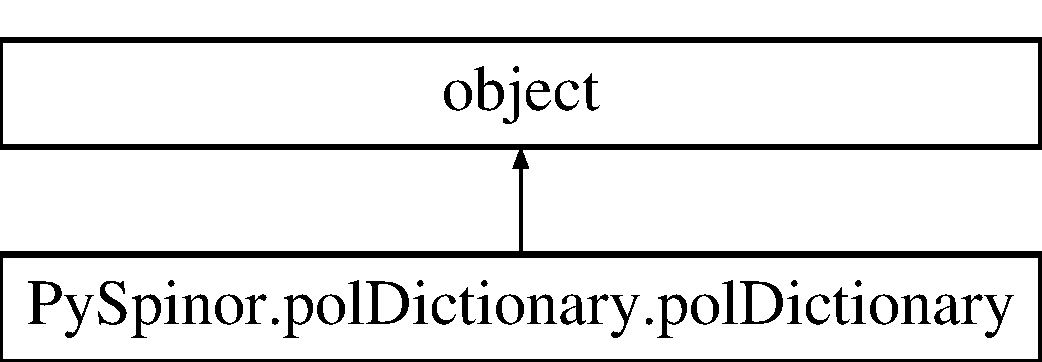
\includegraphics[height=2.000000cm]{class_py_spinor_1_1pol_dictionary_1_1pol_dictionary}
\end{center}
\end{figure}
\subsection*{Public Member Functions}
\begin{DoxyCompactItemize}
\item 
def \hyperlink{class_py_spinor_1_1pol_dictionary_1_1pol_dictionary_aa591099c2d162baef26e4c3a0f1d953e}{\+\_\+\+\_\+init\+\_\+\+\_\+} (self, Dict)
\item 
def \hyperlink{class_py_spinor_1_1pol_dictionary_1_1pol_dictionary_a42794ddf8460d756c5431d6700e7123b}{real} (self)
\item 
def \hyperlink{class_py_spinor_1_1pol_dictionary_1_1pol_dictionary_a704983b1069c410cebb66b83f5449c07}{imag} (self)
\item 
def \hyperlink{class_py_spinor_1_1pol_dictionary_1_1pol_dictionary_a892916dbb6cc54e0c365903e37abf3a9}{zero\+Checker} (self)
\begin{DoxyCompactList}\small\item\em Zero(ish) checker to fix screwed up numerics where things are basically zero but not quite. \end{DoxyCompactList}\item 
def \hyperlink{class_py_spinor_1_1pol_dictionary_1_1pol_dictionary_adccb979d3dcd442690a49ad3ba6e4e23}{\+\_\+\+\_\+call\+\_\+\+\_\+} (self, index)
\begin{DoxyCompactList}\small\item\em Define functor behaviour. \end{DoxyCompactList}\item 
def \hyperlink{class_py_spinor_1_1pol_dictionary_1_1pol_dictionary_a7575411d14bf8c5e4a2d58efe4d175b5}{\+\_\+\+\_\+getitem\+\_\+\+\_\+} (self, i)
\item 
def \hyperlink{class_py_spinor_1_1pol_dictionary_1_1pol_dictionary_ac1d4dc87c1027660422a4af2d46fd78f}{\+\_\+\+\_\+neg\+\_\+\+\_\+} (self)
\item 
def \hyperlink{class_py_spinor_1_1pol_dictionary_1_1pol_dictionary_a2fc7e0be7463d98e2510430261990f50}{\+\_\+\+\_\+pos\+\_\+\+\_\+} (self)
\item 
def \hyperlink{class_py_spinor_1_1pol_dictionary_1_1pol_dictionary_a2c44d12d920ba64d314e10d8827604bf}{\+\_\+\+\_\+iadd\+\_\+\+\_\+} (self, other)
\item 
def \hyperlink{class_py_spinor_1_1pol_dictionary_1_1pol_dictionary_ade193f2738984f6a3df528b64690435a}{\+\_\+\+\_\+str\+\_\+\+\_\+} (self)
\item 
def \hyperlink{class_py_spinor_1_1pol_dictionary_1_1pol_dictionary_a94a6ab60c306097e4df90cf20ff68049}{\+\_\+\+\_\+pow\+\_\+\+\_\+} (self, other)
\item 
def \hyperlink{class_py_spinor_1_1pol_dictionary_1_1pol_dictionary_ae0daee8a58d2276a21361b485d116d16}{\+\_\+\+\_\+eq\+\_\+\+\_\+} (self, other)
\item 
def \hyperlink{class_py_spinor_1_1pol_dictionary_1_1pol_dictionary_ac768f267649ef1eb18069e05b01523bf}{\+\_\+\+\_\+add\+\_\+\+\_\+} (self, other)
\item 
def \hyperlink{class_py_spinor_1_1pol_dictionary_1_1pol_dictionary_ae28a8853b036efc88bdf3088fe1a319f}{\+\_\+\+\_\+sub\+\_\+\+\_\+} (self, other)
\item 
def \hyperlink{class_py_spinor_1_1pol_dictionary_1_1pol_dictionary_a9bfd6a64b42a35c3c9c048a1fa6340fd}{\+\_\+\+\_\+mul\+\_\+\+\_\+} (self, other)
\item 
def \hyperlink{class_py_spinor_1_1pol_dictionary_1_1pol_dictionary_a678e776af32f540e70b5d2731885580b}{\+\_\+\+\_\+rmul\+\_\+\+\_\+} (self, other)
\item 
def \hyperlink{class_py_spinor_1_1pol_dictionary_1_1pol_dictionary_ac36e04fe18bd3b018360c2520cbf9476}{\+\_\+\+\_\+div\+\_\+\+\_\+} (self, other)
\item 
def \hyperlink{class_py_spinor_1_1pol_dictionary_1_1pol_dictionary_a727a579d4b80d6e9086d6972be9481d2}{dot} (self, other)
\item 
def \hyperlink{class_py_spinor_1_1pol_dictionary_1_1pol_dictionary_acca12ba92e7d4582d580f9d49afddc0d}{conjugate} (self)
\item 
def \hyperlink{class_py_spinor_1_1pol_dictionary_1_1pol_dictionary_a18adf99ec4125f4bca8b6435ac893c75}{set\+Polarisations} (self, List)
\item 
def \hyperlink{class_py_spinor_1_1pol_dictionary_1_1pol_dictionary_ad6894204400171c538f4b1266acfed28}{get\+Polarisations}
\end{DoxyCompactItemize}
\subsection*{Public Attributes}
\begin{DoxyCompactItemize}
\item 
\hyperlink{class_py_spinor_1_1pol_dictionary_1_1pol_dictionary_a4af4ee4e42c9fc945e688e94afc69222}{polarisations}
\end{DoxyCompactItemize}
\subsection*{Static Public Attributes}
\begin{DoxyCompactItemize}
\item 
\hyperlink{class_py_spinor_1_1pol_dictionary_1_1pol_dictionary_aa8533ad7b225385b3d7463ff598a594a}{Init} = False
\item 
\hyperlink{class_py_spinor_1_1pol_dictionary_1_1pol_dictionary_a2997e213a191212d4e76e02fe2c79440}{base\+Dict} = None
\end{DoxyCompactItemize}


\subsection{Detailed Description}
A functor class whick holds an item (a current or a \hyperlink{namespace_py_spinor_1_1_lorentz_vector}{Lorentz\+Vector}, ...) for each polarisation in the problem. 

\subsection{Constructor \& Destructor Documentation}
\hypertarget{class_py_spinor_1_1pol_dictionary_1_1pol_dictionary_aa591099c2d162baef26e4c3a0f1d953e}{}\index{Py\+Spinor\+::pol\+Dictionary\+::pol\+Dictionary@{Py\+Spinor\+::pol\+Dictionary\+::pol\+Dictionary}!\+\_\+\+\_\+init\+\_\+\+\_\+@{\+\_\+\+\_\+init\+\_\+\+\_\+}}
\index{\+\_\+\+\_\+init\+\_\+\+\_\+@{\+\_\+\+\_\+init\+\_\+\+\_\+}!Py\+Spinor\+::pol\+Dictionary\+::pol\+Dictionary@{Py\+Spinor\+::pol\+Dictionary\+::pol\+Dictionary}}
\subsubsection[{\+\_\+\+\_\+init\+\_\+\+\_\+}]{\setlength{\rightskip}{0pt plus 5cm}def Py\+Spinor.\+pol\+Dictionary.\+pol\+Dictionary.\+\_\+\+\_\+init\+\_\+\+\_\+ (
\begin{DoxyParamCaption}
\item[{}]{self, }
\item[{}]{Dict}
\end{DoxyParamCaption}
)}\label{class_py_spinor_1_1pol_dictionary_1_1pol_dictionary_aa591099c2d162baef26e4c3a0f1d953e}


\subsection{Member Function Documentation}
\hypertarget{class_py_spinor_1_1pol_dictionary_1_1pol_dictionary_ac768f267649ef1eb18069e05b01523bf}{}\index{Py\+Spinor\+::pol\+Dictionary\+::pol\+Dictionary@{Py\+Spinor\+::pol\+Dictionary\+::pol\+Dictionary}!\+\_\+\+\_\+add\+\_\+\+\_\+@{\+\_\+\+\_\+add\+\_\+\+\_\+}}
\index{\+\_\+\+\_\+add\+\_\+\+\_\+@{\+\_\+\+\_\+add\+\_\+\+\_\+}!Py\+Spinor\+::pol\+Dictionary\+::pol\+Dictionary@{Py\+Spinor\+::pol\+Dictionary\+::pol\+Dictionary}}
\subsubsection[{\+\_\+\+\_\+add\+\_\+\+\_\+}]{\setlength{\rightskip}{0pt plus 5cm}def Py\+Spinor.\+pol\+Dictionary.\+pol\+Dictionary.\+\_\+\+\_\+add\+\_\+\+\_\+ (
\begin{DoxyParamCaption}
\item[{}]{self, }
\item[{}]{other}
\end{DoxyParamCaption}
)}\label{class_py_spinor_1_1pol_dictionary_1_1pol_dictionary_ac768f267649ef1eb18069e05b01523bf}
\hypertarget{class_py_spinor_1_1pol_dictionary_1_1pol_dictionary_adccb979d3dcd442690a49ad3ba6e4e23}{}\index{Py\+Spinor\+::pol\+Dictionary\+::pol\+Dictionary@{Py\+Spinor\+::pol\+Dictionary\+::pol\+Dictionary}!\+\_\+\+\_\+call\+\_\+\+\_\+@{\+\_\+\+\_\+call\+\_\+\+\_\+}}
\index{\+\_\+\+\_\+call\+\_\+\+\_\+@{\+\_\+\+\_\+call\+\_\+\+\_\+}!Py\+Spinor\+::pol\+Dictionary\+::pol\+Dictionary@{Py\+Spinor\+::pol\+Dictionary\+::pol\+Dictionary}}
\subsubsection[{\+\_\+\+\_\+call\+\_\+\+\_\+}]{\setlength{\rightskip}{0pt plus 5cm}def Py\+Spinor.\+pol\+Dictionary.\+pol\+Dictionary.\+\_\+\+\_\+call\+\_\+\+\_\+ (
\begin{DoxyParamCaption}
\item[{}]{self, }
\item[{}]{index}
\end{DoxyParamCaption}
)}\label{class_py_spinor_1_1pol_dictionary_1_1pol_dictionary_adccb979d3dcd442690a49ad3ba6e4e23}


Define functor behaviour. 

\hypertarget{class_py_spinor_1_1pol_dictionary_1_1pol_dictionary_ac36e04fe18bd3b018360c2520cbf9476}{}\index{Py\+Spinor\+::pol\+Dictionary\+::pol\+Dictionary@{Py\+Spinor\+::pol\+Dictionary\+::pol\+Dictionary}!\+\_\+\+\_\+div\+\_\+\+\_\+@{\+\_\+\+\_\+div\+\_\+\+\_\+}}
\index{\+\_\+\+\_\+div\+\_\+\+\_\+@{\+\_\+\+\_\+div\+\_\+\+\_\+}!Py\+Spinor\+::pol\+Dictionary\+::pol\+Dictionary@{Py\+Spinor\+::pol\+Dictionary\+::pol\+Dictionary}}
\subsubsection[{\+\_\+\+\_\+div\+\_\+\+\_\+}]{\setlength{\rightskip}{0pt plus 5cm}def Py\+Spinor.\+pol\+Dictionary.\+pol\+Dictionary.\+\_\+\+\_\+div\+\_\+\+\_\+ (
\begin{DoxyParamCaption}
\item[{}]{self, }
\item[{}]{other}
\end{DoxyParamCaption}
)}\label{class_py_spinor_1_1pol_dictionary_1_1pol_dictionary_ac36e04fe18bd3b018360c2520cbf9476}
\hypertarget{class_py_spinor_1_1pol_dictionary_1_1pol_dictionary_ae0daee8a58d2276a21361b485d116d16}{}\index{Py\+Spinor\+::pol\+Dictionary\+::pol\+Dictionary@{Py\+Spinor\+::pol\+Dictionary\+::pol\+Dictionary}!\+\_\+\+\_\+eq\+\_\+\+\_\+@{\+\_\+\+\_\+eq\+\_\+\+\_\+}}
\index{\+\_\+\+\_\+eq\+\_\+\+\_\+@{\+\_\+\+\_\+eq\+\_\+\+\_\+}!Py\+Spinor\+::pol\+Dictionary\+::pol\+Dictionary@{Py\+Spinor\+::pol\+Dictionary\+::pol\+Dictionary}}
\subsubsection[{\+\_\+\+\_\+eq\+\_\+\+\_\+}]{\setlength{\rightskip}{0pt plus 5cm}def Py\+Spinor.\+pol\+Dictionary.\+pol\+Dictionary.\+\_\+\+\_\+eq\+\_\+\+\_\+ (
\begin{DoxyParamCaption}
\item[{}]{self, }
\item[{}]{other}
\end{DoxyParamCaption}
)}\label{class_py_spinor_1_1pol_dictionary_1_1pol_dictionary_ae0daee8a58d2276a21361b485d116d16}
\hypertarget{class_py_spinor_1_1pol_dictionary_1_1pol_dictionary_a7575411d14bf8c5e4a2d58efe4d175b5}{}\index{Py\+Spinor\+::pol\+Dictionary\+::pol\+Dictionary@{Py\+Spinor\+::pol\+Dictionary\+::pol\+Dictionary}!\+\_\+\+\_\+getitem\+\_\+\+\_\+@{\+\_\+\+\_\+getitem\+\_\+\+\_\+}}
\index{\+\_\+\+\_\+getitem\+\_\+\+\_\+@{\+\_\+\+\_\+getitem\+\_\+\+\_\+}!Py\+Spinor\+::pol\+Dictionary\+::pol\+Dictionary@{Py\+Spinor\+::pol\+Dictionary\+::pol\+Dictionary}}
\subsubsection[{\+\_\+\+\_\+getitem\+\_\+\+\_\+}]{\setlength{\rightskip}{0pt plus 5cm}def Py\+Spinor.\+pol\+Dictionary.\+pol\+Dictionary.\+\_\+\+\_\+getitem\+\_\+\+\_\+ (
\begin{DoxyParamCaption}
\item[{}]{self, }
\item[{}]{i}
\end{DoxyParamCaption}
)}\label{class_py_spinor_1_1pol_dictionary_1_1pol_dictionary_a7575411d14bf8c5e4a2d58efe4d175b5}
\hypertarget{class_py_spinor_1_1pol_dictionary_1_1pol_dictionary_a2c44d12d920ba64d314e10d8827604bf}{}\index{Py\+Spinor\+::pol\+Dictionary\+::pol\+Dictionary@{Py\+Spinor\+::pol\+Dictionary\+::pol\+Dictionary}!\+\_\+\+\_\+iadd\+\_\+\+\_\+@{\+\_\+\+\_\+iadd\+\_\+\+\_\+}}
\index{\+\_\+\+\_\+iadd\+\_\+\+\_\+@{\+\_\+\+\_\+iadd\+\_\+\+\_\+}!Py\+Spinor\+::pol\+Dictionary\+::pol\+Dictionary@{Py\+Spinor\+::pol\+Dictionary\+::pol\+Dictionary}}
\subsubsection[{\+\_\+\+\_\+iadd\+\_\+\+\_\+}]{\setlength{\rightskip}{0pt plus 5cm}def Py\+Spinor.\+pol\+Dictionary.\+pol\+Dictionary.\+\_\+\+\_\+iadd\+\_\+\+\_\+ (
\begin{DoxyParamCaption}
\item[{}]{self, }
\item[{}]{other}
\end{DoxyParamCaption}
)}\label{class_py_spinor_1_1pol_dictionary_1_1pol_dictionary_a2c44d12d920ba64d314e10d8827604bf}
\hypertarget{class_py_spinor_1_1pol_dictionary_1_1pol_dictionary_a9bfd6a64b42a35c3c9c048a1fa6340fd}{}\index{Py\+Spinor\+::pol\+Dictionary\+::pol\+Dictionary@{Py\+Spinor\+::pol\+Dictionary\+::pol\+Dictionary}!\+\_\+\+\_\+mul\+\_\+\+\_\+@{\+\_\+\+\_\+mul\+\_\+\+\_\+}}
\index{\+\_\+\+\_\+mul\+\_\+\+\_\+@{\+\_\+\+\_\+mul\+\_\+\+\_\+}!Py\+Spinor\+::pol\+Dictionary\+::pol\+Dictionary@{Py\+Spinor\+::pol\+Dictionary\+::pol\+Dictionary}}
\subsubsection[{\+\_\+\+\_\+mul\+\_\+\+\_\+}]{\setlength{\rightskip}{0pt plus 5cm}def Py\+Spinor.\+pol\+Dictionary.\+pol\+Dictionary.\+\_\+\+\_\+mul\+\_\+\+\_\+ (
\begin{DoxyParamCaption}
\item[{}]{self, }
\item[{}]{other}
\end{DoxyParamCaption}
)}\label{class_py_spinor_1_1pol_dictionary_1_1pol_dictionary_a9bfd6a64b42a35c3c9c048a1fa6340fd}
\hypertarget{class_py_spinor_1_1pol_dictionary_1_1pol_dictionary_ac1d4dc87c1027660422a4af2d46fd78f}{}\index{Py\+Spinor\+::pol\+Dictionary\+::pol\+Dictionary@{Py\+Spinor\+::pol\+Dictionary\+::pol\+Dictionary}!\+\_\+\+\_\+neg\+\_\+\+\_\+@{\+\_\+\+\_\+neg\+\_\+\+\_\+}}
\index{\+\_\+\+\_\+neg\+\_\+\+\_\+@{\+\_\+\+\_\+neg\+\_\+\+\_\+}!Py\+Spinor\+::pol\+Dictionary\+::pol\+Dictionary@{Py\+Spinor\+::pol\+Dictionary\+::pol\+Dictionary}}
\subsubsection[{\+\_\+\+\_\+neg\+\_\+\+\_\+}]{\setlength{\rightskip}{0pt plus 5cm}def Py\+Spinor.\+pol\+Dictionary.\+pol\+Dictionary.\+\_\+\+\_\+neg\+\_\+\+\_\+ (
\begin{DoxyParamCaption}
\item[{}]{self}
\end{DoxyParamCaption}
)}\label{class_py_spinor_1_1pol_dictionary_1_1pol_dictionary_ac1d4dc87c1027660422a4af2d46fd78f}
\hypertarget{class_py_spinor_1_1pol_dictionary_1_1pol_dictionary_a2fc7e0be7463d98e2510430261990f50}{}\index{Py\+Spinor\+::pol\+Dictionary\+::pol\+Dictionary@{Py\+Spinor\+::pol\+Dictionary\+::pol\+Dictionary}!\+\_\+\+\_\+pos\+\_\+\+\_\+@{\+\_\+\+\_\+pos\+\_\+\+\_\+}}
\index{\+\_\+\+\_\+pos\+\_\+\+\_\+@{\+\_\+\+\_\+pos\+\_\+\+\_\+}!Py\+Spinor\+::pol\+Dictionary\+::pol\+Dictionary@{Py\+Spinor\+::pol\+Dictionary\+::pol\+Dictionary}}
\subsubsection[{\+\_\+\+\_\+pos\+\_\+\+\_\+}]{\setlength{\rightskip}{0pt plus 5cm}def Py\+Spinor.\+pol\+Dictionary.\+pol\+Dictionary.\+\_\+\+\_\+pos\+\_\+\+\_\+ (
\begin{DoxyParamCaption}
\item[{}]{self}
\end{DoxyParamCaption}
)}\label{class_py_spinor_1_1pol_dictionary_1_1pol_dictionary_a2fc7e0be7463d98e2510430261990f50}
\hypertarget{class_py_spinor_1_1pol_dictionary_1_1pol_dictionary_a94a6ab60c306097e4df90cf20ff68049}{}\index{Py\+Spinor\+::pol\+Dictionary\+::pol\+Dictionary@{Py\+Spinor\+::pol\+Dictionary\+::pol\+Dictionary}!\+\_\+\+\_\+pow\+\_\+\+\_\+@{\+\_\+\+\_\+pow\+\_\+\+\_\+}}
\index{\+\_\+\+\_\+pow\+\_\+\+\_\+@{\+\_\+\+\_\+pow\+\_\+\+\_\+}!Py\+Spinor\+::pol\+Dictionary\+::pol\+Dictionary@{Py\+Spinor\+::pol\+Dictionary\+::pol\+Dictionary}}
\subsubsection[{\+\_\+\+\_\+pow\+\_\+\+\_\+}]{\setlength{\rightskip}{0pt plus 5cm}def Py\+Spinor.\+pol\+Dictionary.\+pol\+Dictionary.\+\_\+\+\_\+pow\+\_\+\+\_\+ (
\begin{DoxyParamCaption}
\item[{}]{self, }
\item[{}]{other}
\end{DoxyParamCaption}
)}\label{class_py_spinor_1_1pol_dictionary_1_1pol_dictionary_a94a6ab60c306097e4df90cf20ff68049}
\hypertarget{class_py_spinor_1_1pol_dictionary_1_1pol_dictionary_a678e776af32f540e70b5d2731885580b}{}\index{Py\+Spinor\+::pol\+Dictionary\+::pol\+Dictionary@{Py\+Spinor\+::pol\+Dictionary\+::pol\+Dictionary}!\+\_\+\+\_\+rmul\+\_\+\+\_\+@{\+\_\+\+\_\+rmul\+\_\+\+\_\+}}
\index{\+\_\+\+\_\+rmul\+\_\+\+\_\+@{\+\_\+\+\_\+rmul\+\_\+\+\_\+}!Py\+Spinor\+::pol\+Dictionary\+::pol\+Dictionary@{Py\+Spinor\+::pol\+Dictionary\+::pol\+Dictionary}}
\subsubsection[{\+\_\+\+\_\+rmul\+\_\+\+\_\+}]{\setlength{\rightskip}{0pt plus 5cm}def Py\+Spinor.\+pol\+Dictionary.\+pol\+Dictionary.\+\_\+\+\_\+rmul\+\_\+\+\_\+ (
\begin{DoxyParamCaption}
\item[{}]{self, }
\item[{}]{other}
\end{DoxyParamCaption}
)}\label{class_py_spinor_1_1pol_dictionary_1_1pol_dictionary_a678e776af32f540e70b5d2731885580b}
\hypertarget{class_py_spinor_1_1pol_dictionary_1_1pol_dictionary_ade193f2738984f6a3df528b64690435a}{}\index{Py\+Spinor\+::pol\+Dictionary\+::pol\+Dictionary@{Py\+Spinor\+::pol\+Dictionary\+::pol\+Dictionary}!\+\_\+\+\_\+str\+\_\+\+\_\+@{\+\_\+\+\_\+str\+\_\+\+\_\+}}
\index{\+\_\+\+\_\+str\+\_\+\+\_\+@{\+\_\+\+\_\+str\+\_\+\+\_\+}!Py\+Spinor\+::pol\+Dictionary\+::pol\+Dictionary@{Py\+Spinor\+::pol\+Dictionary\+::pol\+Dictionary}}
\subsubsection[{\+\_\+\+\_\+str\+\_\+\+\_\+}]{\setlength{\rightskip}{0pt plus 5cm}def Py\+Spinor.\+pol\+Dictionary.\+pol\+Dictionary.\+\_\+\+\_\+str\+\_\+\+\_\+ (
\begin{DoxyParamCaption}
\item[{}]{self}
\end{DoxyParamCaption}
)}\label{class_py_spinor_1_1pol_dictionary_1_1pol_dictionary_ade193f2738984f6a3df528b64690435a}
\hypertarget{class_py_spinor_1_1pol_dictionary_1_1pol_dictionary_ae28a8853b036efc88bdf3088fe1a319f}{}\index{Py\+Spinor\+::pol\+Dictionary\+::pol\+Dictionary@{Py\+Spinor\+::pol\+Dictionary\+::pol\+Dictionary}!\+\_\+\+\_\+sub\+\_\+\+\_\+@{\+\_\+\+\_\+sub\+\_\+\+\_\+}}
\index{\+\_\+\+\_\+sub\+\_\+\+\_\+@{\+\_\+\+\_\+sub\+\_\+\+\_\+}!Py\+Spinor\+::pol\+Dictionary\+::pol\+Dictionary@{Py\+Spinor\+::pol\+Dictionary\+::pol\+Dictionary}}
\subsubsection[{\+\_\+\+\_\+sub\+\_\+\+\_\+}]{\setlength{\rightskip}{0pt plus 5cm}def Py\+Spinor.\+pol\+Dictionary.\+pol\+Dictionary.\+\_\+\+\_\+sub\+\_\+\+\_\+ (
\begin{DoxyParamCaption}
\item[{}]{self, }
\item[{}]{other}
\end{DoxyParamCaption}
)}\label{class_py_spinor_1_1pol_dictionary_1_1pol_dictionary_ae28a8853b036efc88bdf3088fe1a319f}
\hypertarget{class_py_spinor_1_1pol_dictionary_1_1pol_dictionary_acca12ba92e7d4582d580f9d49afddc0d}{}\index{Py\+Spinor\+::pol\+Dictionary\+::pol\+Dictionary@{Py\+Spinor\+::pol\+Dictionary\+::pol\+Dictionary}!conjugate@{conjugate}}
\index{conjugate@{conjugate}!Py\+Spinor\+::pol\+Dictionary\+::pol\+Dictionary@{Py\+Spinor\+::pol\+Dictionary\+::pol\+Dictionary}}
\subsubsection[{conjugate}]{\setlength{\rightskip}{0pt plus 5cm}def Py\+Spinor.\+pol\+Dictionary.\+pol\+Dictionary.\+conjugate (
\begin{DoxyParamCaption}
\item[{}]{self}
\end{DoxyParamCaption}
)}\label{class_py_spinor_1_1pol_dictionary_1_1pol_dictionary_acca12ba92e7d4582d580f9d49afddc0d}
\hypertarget{class_py_spinor_1_1pol_dictionary_1_1pol_dictionary_a727a579d4b80d6e9086d6972be9481d2}{}\index{Py\+Spinor\+::pol\+Dictionary\+::pol\+Dictionary@{Py\+Spinor\+::pol\+Dictionary\+::pol\+Dictionary}!dot@{dot}}
\index{dot@{dot}!Py\+Spinor\+::pol\+Dictionary\+::pol\+Dictionary@{Py\+Spinor\+::pol\+Dictionary\+::pol\+Dictionary}}
\subsubsection[{dot}]{\setlength{\rightskip}{0pt plus 5cm}def Py\+Spinor.\+pol\+Dictionary.\+pol\+Dictionary.\+dot (
\begin{DoxyParamCaption}
\item[{}]{self, }
\item[{}]{other}
\end{DoxyParamCaption}
)}\label{class_py_spinor_1_1pol_dictionary_1_1pol_dictionary_a727a579d4b80d6e9086d6972be9481d2}
\hypertarget{class_py_spinor_1_1pol_dictionary_1_1pol_dictionary_ad6894204400171c538f4b1266acfed28}{}\index{Py\+Spinor\+::pol\+Dictionary\+::pol\+Dictionary@{Py\+Spinor\+::pol\+Dictionary\+::pol\+Dictionary}!get\+Polarisations@{get\+Polarisations}}
\index{get\+Polarisations@{get\+Polarisations}!Py\+Spinor\+::pol\+Dictionary\+::pol\+Dictionary@{Py\+Spinor\+::pol\+Dictionary\+::pol\+Dictionary}}
\subsubsection[{get\+Polarisations}]{\setlength{\rightskip}{0pt plus 5cm}def Py\+Spinor.\+pol\+Dictionary.\+pol\+Dictionary.\+get\+Polarisations (
\begin{DoxyParamCaption}
\item[{}]{self, }
\item[{}]{List = {\ttfamily False}, }
\item[{}]{Force\+New = {\ttfamily False}, }
\item[{}]{Fixed = {\ttfamily None}}
\end{DoxyParamCaption}
)}\label{class_py_spinor_1_1pol_dictionary_1_1pol_dictionary_ad6894204400171c538f4b1266acfed28}
\hypertarget{class_py_spinor_1_1pol_dictionary_1_1pol_dictionary_a704983b1069c410cebb66b83f5449c07}{}\index{Py\+Spinor\+::pol\+Dictionary\+::pol\+Dictionary@{Py\+Spinor\+::pol\+Dictionary\+::pol\+Dictionary}!imag@{imag}}
\index{imag@{imag}!Py\+Spinor\+::pol\+Dictionary\+::pol\+Dictionary@{Py\+Spinor\+::pol\+Dictionary\+::pol\+Dictionary}}
\subsubsection[{imag}]{\setlength{\rightskip}{0pt plus 5cm}def Py\+Spinor.\+pol\+Dictionary.\+pol\+Dictionary.\+imag (
\begin{DoxyParamCaption}
\item[{}]{self}
\end{DoxyParamCaption}
)}\label{class_py_spinor_1_1pol_dictionary_1_1pol_dictionary_a704983b1069c410cebb66b83f5449c07}
\hypertarget{class_py_spinor_1_1pol_dictionary_1_1pol_dictionary_a42794ddf8460d756c5431d6700e7123b}{}\index{Py\+Spinor\+::pol\+Dictionary\+::pol\+Dictionary@{Py\+Spinor\+::pol\+Dictionary\+::pol\+Dictionary}!real@{real}}
\index{real@{real}!Py\+Spinor\+::pol\+Dictionary\+::pol\+Dictionary@{Py\+Spinor\+::pol\+Dictionary\+::pol\+Dictionary}}
\subsubsection[{real}]{\setlength{\rightskip}{0pt plus 5cm}def Py\+Spinor.\+pol\+Dictionary.\+pol\+Dictionary.\+real (
\begin{DoxyParamCaption}
\item[{}]{self}
\end{DoxyParamCaption}
)}\label{class_py_spinor_1_1pol_dictionary_1_1pol_dictionary_a42794ddf8460d756c5431d6700e7123b}
\hypertarget{class_py_spinor_1_1pol_dictionary_1_1pol_dictionary_a18adf99ec4125f4bca8b6435ac893c75}{}\index{Py\+Spinor\+::pol\+Dictionary\+::pol\+Dictionary@{Py\+Spinor\+::pol\+Dictionary\+::pol\+Dictionary}!set\+Polarisations@{set\+Polarisations}}
\index{set\+Polarisations@{set\+Polarisations}!Py\+Spinor\+::pol\+Dictionary\+::pol\+Dictionary@{Py\+Spinor\+::pol\+Dictionary\+::pol\+Dictionary}}
\subsubsection[{set\+Polarisations}]{\setlength{\rightskip}{0pt plus 5cm}def Py\+Spinor.\+pol\+Dictionary.\+pol\+Dictionary.\+set\+Polarisations (
\begin{DoxyParamCaption}
\item[{}]{self, }
\item[{}]{List}
\end{DoxyParamCaption}
)}\label{class_py_spinor_1_1pol_dictionary_1_1pol_dictionary_a18adf99ec4125f4bca8b6435ac893c75}
\hypertarget{class_py_spinor_1_1pol_dictionary_1_1pol_dictionary_a892916dbb6cc54e0c365903e37abf3a9}{}\index{Py\+Spinor\+::pol\+Dictionary\+::pol\+Dictionary@{Py\+Spinor\+::pol\+Dictionary\+::pol\+Dictionary}!zero\+Checker@{zero\+Checker}}
\index{zero\+Checker@{zero\+Checker}!Py\+Spinor\+::pol\+Dictionary\+::pol\+Dictionary@{Py\+Spinor\+::pol\+Dictionary\+::pol\+Dictionary}}
\subsubsection[{zero\+Checker}]{\setlength{\rightskip}{0pt plus 5cm}def Py\+Spinor.\+pol\+Dictionary.\+pol\+Dictionary.\+zero\+Checker (
\begin{DoxyParamCaption}
\item[{}]{self}
\end{DoxyParamCaption}
)}\label{class_py_spinor_1_1pol_dictionary_1_1pol_dictionary_a892916dbb6cc54e0c365903e37abf3a9}


Zero(ish) checker to fix screwed up numerics where things are basically zero but not quite. 



\subsection{Member Data Documentation}
\hypertarget{class_py_spinor_1_1pol_dictionary_1_1pol_dictionary_a2997e213a191212d4e76e02fe2c79440}{}\index{Py\+Spinor\+::pol\+Dictionary\+::pol\+Dictionary@{Py\+Spinor\+::pol\+Dictionary\+::pol\+Dictionary}!base\+Dict@{base\+Dict}}
\index{base\+Dict@{base\+Dict}!Py\+Spinor\+::pol\+Dictionary\+::pol\+Dictionary@{Py\+Spinor\+::pol\+Dictionary\+::pol\+Dictionary}}
\subsubsection[{base\+Dict}]{\setlength{\rightskip}{0pt plus 5cm}Py\+Spinor.\+pol\+Dictionary.\+pol\+Dictionary.\+base\+Dict = None\hspace{0.3cm}{\ttfamily [static]}}\label{class_py_spinor_1_1pol_dictionary_1_1pol_dictionary_a2997e213a191212d4e76e02fe2c79440}
\hypertarget{class_py_spinor_1_1pol_dictionary_1_1pol_dictionary_aa8533ad7b225385b3d7463ff598a594a}{}\index{Py\+Spinor\+::pol\+Dictionary\+::pol\+Dictionary@{Py\+Spinor\+::pol\+Dictionary\+::pol\+Dictionary}!Init@{Init}}
\index{Init@{Init}!Py\+Spinor\+::pol\+Dictionary\+::pol\+Dictionary@{Py\+Spinor\+::pol\+Dictionary\+::pol\+Dictionary}}
\subsubsection[{Init}]{\setlength{\rightskip}{0pt plus 5cm}Py\+Spinor.\+pol\+Dictionary.\+pol\+Dictionary.\+Init = False\hspace{0.3cm}{\ttfamily [static]}}\label{class_py_spinor_1_1pol_dictionary_1_1pol_dictionary_aa8533ad7b225385b3d7463ff598a594a}
\hypertarget{class_py_spinor_1_1pol_dictionary_1_1pol_dictionary_a4af4ee4e42c9fc945e688e94afc69222}{}\index{Py\+Spinor\+::pol\+Dictionary\+::pol\+Dictionary@{Py\+Spinor\+::pol\+Dictionary\+::pol\+Dictionary}!polarisations@{polarisations}}
\index{polarisations@{polarisations}!Py\+Spinor\+::pol\+Dictionary\+::pol\+Dictionary@{Py\+Spinor\+::pol\+Dictionary\+::pol\+Dictionary}}
\subsubsection[{polarisations}]{\setlength{\rightskip}{0pt plus 5cm}Py\+Spinor.\+pol\+Dictionary.\+pol\+Dictionary.\+polarisations}\label{class_py_spinor_1_1pol_dictionary_1_1pol_dictionary_a4af4ee4e42c9fc945e688e94afc69222}


The documentation for this class was generated from the following file\+:\begin{DoxyCompactItemize}
\item 
Py\+Spinor/\hyperlink{pol_dictionary_8py}{pol\+Dictionary.\+py}\end{DoxyCompactItemize}

\hypertarget{class_py_spinor_1_1_spinor_1_1_spinor_1_1spinor}{}\section{Py\+Spinor.\+Spinor.\+Spinor.\+spinor Class Reference}
\label{class_py_spinor_1_1_spinor_1_1_spinor_1_1spinor}\index{Py\+Spinor.\+Spinor.\+Spinor.\+spinor@{Py\+Spinor.\+Spinor.\+Spinor.\+spinor}}
\subsection*{Public Member Functions}
\begin{DoxyCompactItemize}
\item 
def \hyperlink{class_py_spinor_1_1_spinor_1_1_spinor_1_1spinor_ac0ac1a9c34ee87ffdf28d0ccb75d70f6}{\+\_\+\+\_\+init\+\_\+\+\_\+}
\item 
def \hyperlink{class_py_spinor_1_1_spinor_1_1_spinor_1_1spinor_a25b5c7b4cb11c895cd7d52299e920109}{\+\_\+\+\_\+str\+\_\+\+\_\+} (self)
\item 
def \hyperlink{class_py_spinor_1_1_spinor_1_1_spinor_1_1spinor_aa24c84582fe66fb8c3faf9ac2d154d33}{get\+Polarisation} (self)
\item 
def \hyperlink{class_py_spinor_1_1_spinor_1_1_spinor_1_1spinor_a8978e7ce7a8062bc89a49869f56f6a7d}{get\+Vector} (self)
\item 
def \hyperlink{class_py_spinor_1_1_spinor_1_1_spinor_1_1spinor_a0d17e1251c4f618d0ec774afb81faeee}{bar} (self)
\item 
def \hyperlink{class_py_spinor_1_1_spinor_1_1_spinor_1_1spinor_af465a6725d4bacc98904a549aa3f7d11}{\+\_\+\+\_\+neg\+\_\+\+\_\+} (self)
\item 
def \hyperlink{class_py_spinor_1_1_spinor_1_1_spinor_1_1spinor_a6bbf536bf21e0cf2a07e4303c73005fc}{\+\_\+\+\_\+eq\+\_\+\+\_\+} (self, other)
\item 
def \hyperlink{class_py_spinor_1_1_spinor_1_1_spinor_1_1spinor_abdb11b78abbe44edc5a142bc3bc7a9f3}{\+\_\+\+\_\+add\+\_\+\+\_\+} (self, other)
\begin{DoxyCompactList}\small\item\em Addition. \end{DoxyCompactList}\item 
def \hyperlink{class_py_spinor_1_1_spinor_1_1_spinor_1_1spinor_ab5bdcc99b407f583ccc01b3bb1a8bab1}{\+\_\+\+\_\+sub\+\_\+\+\_\+} (self, other)
\begin{DoxyCompactList}\small\item\em Subtraction. \end{DoxyCompactList}\item 
def \hyperlink{class_py_spinor_1_1_spinor_1_1_spinor_1_1spinor_a5d6546fecf5c0457d02b4a903d0a850b}{\+\_\+\+\_\+radd\+\_\+\+\_\+} (self, other)
\item 
def \hyperlink{class_py_spinor_1_1_spinor_1_1_spinor_1_1spinor_a45fbedd6e65f08c465d791ad08e2e976}{\+\_\+\+\_\+rsub\+\_\+\+\_\+} (self, other)
\item 
def \hyperlink{class_py_spinor_1_1_spinor_1_1_spinor_1_1spinor_a825d92f2532b5bf5e0a1bb2c637e5376}{\+\_\+\+\_\+mul\+\_\+\+\_\+} (self, other)
\item 
def \hyperlink{class_py_spinor_1_1_spinor_1_1_spinor_1_1spinor_a28c2abeb6c45a5d1ba21250be157f7e7}{\+\_\+\+\_\+div\+\_\+\+\_\+} (self, other)
\item 
def \hyperlink{class_py_spinor_1_1_spinor_1_1_spinor_1_1spinor_a0bab993df788244b3901a80c0a395c69}{\+\_\+\+\_\+rmul\+\_\+\+\_\+} (self, other)
\item 
def \hyperlink{class_py_spinor_1_1_spinor_1_1_spinor_1_1spinor_a042d7392fe6ebf7e822971bb3050a3d2}{\+\_\+\+\_\+ne\+\_\+\+\_\+} (self, other)
\end{DoxyCompactItemize}
\subsection*{Public Attributes}
\begin{DoxyCompactItemize}
\item 
\hyperlink{class_py_spinor_1_1_spinor_1_1_spinor_1_1spinor_abe884cc066c6c81bfad50facf0f1abd4}{momentum}
\item 
\hyperlink{class_py_spinor_1_1_spinor_1_1_spinor_1_1spinor_a6d0116dfdbfd42c9593c742d84973e8c}{barred}
\item 
\hyperlink{class_py_spinor_1_1_spinor_1_1_spinor_1_1spinor_a44788846d9426038bd780f129ad388c6}{pol}
\item 
\hyperlink{class_py_spinor_1_1_spinor_1_1_spinor_1_1spinor_ab64828963b1152f66e897919680c082a}{I\+D}
\item 
\hyperlink{class_py_spinor_1_1_spinor_1_1_spinor_1_1spinor_ac1325eb3bbd07e47641e42fc150bed3f}{vector}
\end{DoxyCompactItemize}


\subsection{Constructor \& Destructor Documentation}
\hypertarget{class_py_spinor_1_1_spinor_1_1_spinor_1_1spinor_ac0ac1a9c34ee87ffdf28d0ccb75d70f6}{}\index{Py\+Spinor\+::\+Spinor\+::\+Spinor\+::spinor@{Py\+Spinor\+::\+Spinor\+::\+Spinor\+::spinor}!\+\_\+\+\_\+init\+\_\+\+\_\+@{\+\_\+\+\_\+init\+\_\+\+\_\+}}
\index{\+\_\+\+\_\+init\+\_\+\+\_\+@{\+\_\+\+\_\+init\+\_\+\+\_\+}!Py\+Spinor\+::\+Spinor\+::\+Spinor\+::spinor@{Py\+Spinor\+::\+Spinor\+::\+Spinor\+::spinor}}
\subsubsection[{\+\_\+\+\_\+init\+\_\+\+\_\+}]{\setlength{\rightskip}{0pt plus 5cm}def Py\+Spinor.\+Spinor.\+Spinor.\+spinor.\+\_\+\+\_\+init\+\_\+\+\_\+ (
\begin{DoxyParamCaption}
\item[{}]{self, }
\item[{}]{momentum, }
\item[{}]{pol, }
\item[{}]{barred = {\ttfamily False}, }
\item[{}]{vector = {\ttfamily None}, }
\item[{}]{I\+D = {\ttfamily None}}
\end{DoxyParamCaption}
)}\label{class_py_spinor_1_1_spinor_1_1_spinor_1_1spinor_ac0ac1a9c34ee87ffdf28d0ccb75d70f6}


\subsection{Member Function Documentation}
\hypertarget{class_py_spinor_1_1_spinor_1_1_spinor_1_1spinor_abdb11b78abbe44edc5a142bc3bc7a9f3}{}\index{Py\+Spinor\+::\+Spinor\+::\+Spinor\+::spinor@{Py\+Spinor\+::\+Spinor\+::\+Spinor\+::spinor}!\+\_\+\+\_\+add\+\_\+\+\_\+@{\+\_\+\+\_\+add\+\_\+\+\_\+}}
\index{\+\_\+\+\_\+add\+\_\+\+\_\+@{\+\_\+\+\_\+add\+\_\+\+\_\+}!Py\+Spinor\+::\+Spinor\+::\+Spinor\+::spinor@{Py\+Spinor\+::\+Spinor\+::\+Spinor\+::spinor}}
\subsubsection[{\+\_\+\+\_\+add\+\_\+\+\_\+}]{\setlength{\rightskip}{0pt plus 5cm}def Py\+Spinor.\+Spinor.\+Spinor.\+spinor.\+\_\+\+\_\+add\+\_\+\+\_\+ (
\begin{DoxyParamCaption}
\item[{}]{self, }
\item[{}]{other}
\end{DoxyParamCaption}
)}\label{class_py_spinor_1_1_spinor_1_1_spinor_1_1spinor_abdb11b78abbe44edc5a142bc3bc7a9f3}


Addition. 

\hypertarget{class_py_spinor_1_1_spinor_1_1_spinor_1_1spinor_a28c2abeb6c45a5d1ba21250be157f7e7}{}\index{Py\+Spinor\+::\+Spinor\+::\+Spinor\+::spinor@{Py\+Spinor\+::\+Spinor\+::\+Spinor\+::spinor}!\+\_\+\+\_\+div\+\_\+\+\_\+@{\+\_\+\+\_\+div\+\_\+\+\_\+}}
\index{\+\_\+\+\_\+div\+\_\+\+\_\+@{\+\_\+\+\_\+div\+\_\+\+\_\+}!Py\+Spinor\+::\+Spinor\+::\+Spinor\+::spinor@{Py\+Spinor\+::\+Spinor\+::\+Spinor\+::spinor}}
\subsubsection[{\+\_\+\+\_\+div\+\_\+\+\_\+}]{\setlength{\rightskip}{0pt plus 5cm}def Py\+Spinor.\+Spinor.\+Spinor.\+spinor.\+\_\+\+\_\+div\+\_\+\+\_\+ (
\begin{DoxyParamCaption}
\item[{}]{self, }
\item[{}]{other}
\end{DoxyParamCaption}
)}\label{class_py_spinor_1_1_spinor_1_1_spinor_1_1spinor_a28c2abeb6c45a5d1ba21250be157f7e7}
\hypertarget{class_py_spinor_1_1_spinor_1_1_spinor_1_1spinor_a6bbf536bf21e0cf2a07e4303c73005fc}{}\index{Py\+Spinor\+::\+Spinor\+::\+Spinor\+::spinor@{Py\+Spinor\+::\+Spinor\+::\+Spinor\+::spinor}!\+\_\+\+\_\+eq\+\_\+\+\_\+@{\+\_\+\+\_\+eq\+\_\+\+\_\+}}
\index{\+\_\+\+\_\+eq\+\_\+\+\_\+@{\+\_\+\+\_\+eq\+\_\+\+\_\+}!Py\+Spinor\+::\+Spinor\+::\+Spinor\+::spinor@{Py\+Spinor\+::\+Spinor\+::\+Spinor\+::spinor}}
\subsubsection[{\+\_\+\+\_\+eq\+\_\+\+\_\+}]{\setlength{\rightskip}{0pt plus 5cm}def Py\+Spinor.\+Spinor.\+Spinor.\+spinor.\+\_\+\+\_\+eq\+\_\+\+\_\+ (
\begin{DoxyParamCaption}
\item[{}]{self, }
\item[{}]{other}
\end{DoxyParamCaption}
)}\label{class_py_spinor_1_1_spinor_1_1_spinor_1_1spinor_a6bbf536bf21e0cf2a07e4303c73005fc}
\hypertarget{class_py_spinor_1_1_spinor_1_1_spinor_1_1spinor_a825d92f2532b5bf5e0a1bb2c637e5376}{}\index{Py\+Spinor\+::\+Spinor\+::\+Spinor\+::spinor@{Py\+Spinor\+::\+Spinor\+::\+Spinor\+::spinor}!\+\_\+\+\_\+mul\+\_\+\+\_\+@{\+\_\+\+\_\+mul\+\_\+\+\_\+}}
\index{\+\_\+\+\_\+mul\+\_\+\+\_\+@{\+\_\+\+\_\+mul\+\_\+\+\_\+}!Py\+Spinor\+::\+Spinor\+::\+Spinor\+::spinor@{Py\+Spinor\+::\+Spinor\+::\+Spinor\+::spinor}}
\subsubsection[{\+\_\+\+\_\+mul\+\_\+\+\_\+}]{\setlength{\rightskip}{0pt plus 5cm}def Py\+Spinor.\+Spinor.\+Spinor.\+spinor.\+\_\+\+\_\+mul\+\_\+\+\_\+ (
\begin{DoxyParamCaption}
\item[{}]{self, }
\item[{}]{other}
\end{DoxyParamCaption}
)}\label{class_py_spinor_1_1_spinor_1_1_spinor_1_1spinor_a825d92f2532b5bf5e0a1bb2c637e5376}
\hypertarget{class_py_spinor_1_1_spinor_1_1_spinor_1_1spinor_a042d7392fe6ebf7e822971bb3050a3d2}{}\index{Py\+Spinor\+::\+Spinor\+::\+Spinor\+::spinor@{Py\+Spinor\+::\+Spinor\+::\+Spinor\+::spinor}!\+\_\+\+\_\+ne\+\_\+\+\_\+@{\+\_\+\+\_\+ne\+\_\+\+\_\+}}
\index{\+\_\+\+\_\+ne\+\_\+\+\_\+@{\+\_\+\+\_\+ne\+\_\+\+\_\+}!Py\+Spinor\+::\+Spinor\+::\+Spinor\+::spinor@{Py\+Spinor\+::\+Spinor\+::\+Spinor\+::spinor}}
\subsubsection[{\+\_\+\+\_\+ne\+\_\+\+\_\+}]{\setlength{\rightskip}{0pt plus 5cm}def Py\+Spinor.\+Spinor.\+Spinor.\+spinor.\+\_\+\+\_\+ne\+\_\+\+\_\+ (
\begin{DoxyParamCaption}
\item[{}]{self, }
\item[{}]{other}
\end{DoxyParamCaption}
)}\label{class_py_spinor_1_1_spinor_1_1_spinor_1_1spinor_a042d7392fe6ebf7e822971bb3050a3d2}
\hypertarget{class_py_spinor_1_1_spinor_1_1_spinor_1_1spinor_af465a6725d4bacc98904a549aa3f7d11}{}\index{Py\+Spinor\+::\+Spinor\+::\+Spinor\+::spinor@{Py\+Spinor\+::\+Spinor\+::\+Spinor\+::spinor}!\+\_\+\+\_\+neg\+\_\+\+\_\+@{\+\_\+\+\_\+neg\+\_\+\+\_\+}}
\index{\+\_\+\+\_\+neg\+\_\+\+\_\+@{\+\_\+\+\_\+neg\+\_\+\+\_\+}!Py\+Spinor\+::\+Spinor\+::\+Spinor\+::spinor@{Py\+Spinor\+::\+Spinor\+::\+Spinor\+::spinor}}
\subsubsection[{\+\_\+\+\_\+neg\+\_\+\+\_\+}]{\setlength{\rightskip}{0pt plus 5cm}def Py\+Spinor.\+Spinor.\+Spinor.\+spinor.\+\_\+\+\_\+neg\+\_\+\+\_\+ (
\begin{DoxyParamCaption}
\item[{}]{self}
\end{DoxyParamCaption}
)}\label{class_py_spinor_1_1_spinor_1_1_spinor_1_1spinor_af465a6725d4bacc98904a549aa3f7d11}
\hypertarget{class_py_spinor_1_1_spinor_1_1_spinor_1_1spinor_a5d6546fecf5c0457d02b4a903d0a850b}{}\index{Py\+Spinor\+::\+Spinor\+::\+Spinor\+::spinor@{Py\+Spinor\+::\+Spinor\+::\+Spinor\+::spinor}!\+\_\+\+\_\+radd\+\_\+\+\_\+@{\+\_\+\+\_\+radd\+\_\+\+\_\+}}
\index{\+\_\+\+\_\+radd\+\_\+\+\_\+@{\+\_\+\+\_\+radd\+\_\+\+\_\+}!Py\+Spinor\+::\+Spinor\+::\+Spinor\+::spinor@{Py\+Spinor\+::\+Spinor\+::\+Spinor\+::spinor}}
\subsubsection[{\+\_\+\+\_\+radd\+\_\+\+\_\+}]{\setlength{\rightskip}{0pt plus 5cm}def Py\+Spinor.\+Spinor.\+Spinor.\+spinor.\+\_\+\+\_\+radd\+\_\+\+\_\+ (
\begin{DoxyParamCaption}
\item[{}]{self, }
\item[{}]{other}
\end{DoxyParamCaption}
)}\label{class_py_spinor_1_1_spinor_1_1_spinor_1_1spinor_a5d6546fecf5c0457d02b4a903d0a850b}
\hypertarget{class_py_spinor_1_1_spinor_1_1_spinor_1_1spinor_a0bab993df788244b3901a80c0a395c69}{}\index{Py\+Spinor\+::\+Spinor\+::\+Spinor\+::spinor@{Py\+Spinor\+::\+Spinor\+::\+Spinor\+::spinor}!\+\_\+\+\_\+rmul\+\_\+\+\_\+@{\+\_\+\+\_\+rmul\+\_\+\+\_\+}}
\index{\+\_\+\+\_\+rmul\+\_\+\+\_\+@{\+\_\+\+\_\+rmul\+\_\+\+\_\+}!Py\+Spinor\+::\+Spinor\+::\+Spinor\+::spinor@{Py\+Spinor\+::\+Spinor\+::\+Spinor\+::spinor}}
\subsubsection[{\+\_\+\+\_\+rmul\+\_\+\+\_\+}]{\setlength{\rightskip}{0pt plus 5cm}def Py\+Spinor.\+Spinor.\+Spinor.\+spinor.\+\_\+\+\_\+rmul\+\_\+\+\_\+ (
\begin{DoxyParamCaption}
\item[{}]{self, }
\item[{}]{other}
\end{DoxyParamCaption}
)}\label{class_py_spinor_1_1_spinor_1_1_spinor_1_1spinor_a0bab993df788244b3901a80c0a395c69}
\hypertarget{class_py_spinor_1_1_spinor_1_1_spinor_1_1spinor_a45fbedd6e65f08c465d791ad08e2e976}{}\index{Py\+Spinor\+::\+Spinor\+::\+Spinor\+::spinor@{Py\+Spinor\+::\+Spinor\+::\+Spinor\+::spinor}!\+\_\+\+\_\+rsub\+\_\+\+\_\+@{\+\_\+\+\_\+rsub\+\_\+\+\_\+}}
\index{\+\_\+\+\_\+rsub\+\_\+\+\_\+@{\+\_\+\+\_\+rsub\+\_\+\+\_\+}!Py\+Spinor\+::\+Spinor\+::\+Spinor\+::spinor@{Py\+Spinor\+::\+Spinor\+::\+Spinor\+::spinor}}
\subsubsection[{\+\_\+\+\_\+rsub\+\_\+\+\_\+}]{\setlength{\rightskip}{0pt plus 5cm}def Py\+Spinor.\+Spinor.\+Spinor.\+spinor.\+\_\+\+\_\+rsub\+\_\+\+\_\+ (
\begin{DoxyParamCaption}
\item[{}]{self, }
\item[{}]{other}
\end{DoxyParamCaption}
)}\label{class_py_spinor_1_1_spinor_1_1_spinor_1_1spinor_a45fbedd6e65f08c465d791ad08e2e976}
\hypertarget{class_py_spinor_1_1_spinor_1_1_spinor_1_1spinor_a25b5c7b4cb11c895cd7d52299e920109}{}\index{Py\+Spinor\+::\+Spinor\+::\+Spinor\+::spinor@{Py\+Spinor\+::\+Spinor\+::\+Spinor\+::spinor}!\+\_\+\+\_\+str\+\_\+\+\_\+@{\+\_\+\+\_\+str\+\_\+\+\_\+}}
\index{\+\_\+\+\_\+str\+\_\+\+\_\+@{\+\_\+\+\_\+str\+\_\+\+\_\+}!Py\+Spinor\+::\+Spinor\+::\+Spinor\+::spinor@{Py\+Spinor\+::\+Spinor\+::\+Spinor\+::spinor}}
\subsubsection[{\+\_\+\+\_\+str\+\_\+\+\_\+}]{\setlength{\rightskip}{0pt plus 5cm}def Py\+Spinor.\+Spinor.\+Spinor.\+spinor.\+\_\+\+\_\+str\+\_\+\+\_\+ (
\begin{DoxyParamCaption}
\item[{}]{self}
\end{DoxyParamCaption}
)}\label{class_py_spinor_1_1_spinor_1_1_spinor_1_1spinor_a25b5c7b4cb11c895cd7d52299e920109}
\hypertarget{class_py_spinor_1_1_spinor_1_1_spinor_1_1spinor_ab5bdcc99b407f583ccc01b3bb1a8bab1}{}\index{Py\+Spinor\+::\+Spinor\+::\+Spinor\+::spinor@{Py\+Spinor\+::\+Spinor\+::\+Spinor\+::spinor}!\+\_\+\+\_\+sub\+\_\+\+\_\+@{\+\_\+\+\_\+sub\+\_\+\+\_\+}}
\index{\+\_\+\+\_\+sub\+\_\+\+\_\+@{\+\_\+\+\_\+sub\+\_\+\+\_\+}!Py\+Spinor\+::\+Spinor\+::\+Spinor\+::spinor@{Py\+Spinor\+::\+Spinor\+::\+Spinor\+::spinor}}
\subsubsection[{\+\_\+\+\_\+sub\+\_\+\+\_\+}]{\setlength{\rightskip}{0pt plus 5cm}def Py\+Spinor.\+Spinor.\+Spinor.\+spinor.\+\_\+\+\_\+sub\+\_\+\+\_\+ (
\begin{DoxyParamCaption}
\item[{}]{self, }
\item[{}]{other}
\end{DoxyParamCaption}
)}\label{class_py_spinor_1_1_spinor_1_1_spinor_1_1spinor_ab5bdcc99b407f583ccc01b3bb1a8bab1}


Subtraction. 

\hypertarget{class_py_spinor_1_1_spinor_1_1_spinor_1_1spinor_a0d17e1251c4f618d0ec774afb81faeee}{}\index{Py\+Spinor\+::\+Spinor\+::\+Spinor\+::spinor@{Py\+Spinor\+::\+Spinor\+::\+Spinor\+::spinor}!bar@{bar}}
\index{bar@{bar}!Py\+Spinor\+::\+Spinor\+::\+Spinor\+::spinor@{Py\+Spinor\+::\+Spinor\+::\+Spinor\+::spinor}}
\subsubsection[{bar}]{\setlength{\rightskip}{0pt plus 5cm}def Py\+Spinor.\+Spinor.\+Spinor.\+spinor.\+bar (
\begin{DoxyParamCaption}
\item[{}]{self}
\end{DoxyParamCaption}
)}\label{class_py_spinor_1_1_spinor_1_1_spinor_1_1spinor_a0d17e1251c4f618d0ec774afb81faeee}
\hypertarget{class_py_spinor_1_1_spinor_1_1_spinor_1_1spinor_aa24c84582fe66fb8c3faf9ac2d154d33}{}\index{Py\+Spinor\+::\+Spinor\+::\+Spinor\+::spinor@{Py\+Spinor\+::\+Spinor\+::\+Spinor\+::spinor}!get\+Polarisation@{get\+Polarisation}}
\index{get\+Polarisation@{get\+Polarisation}!Py\+Spinor\+::\+Spinor\+::\+Spinor\+::spinor@{Py\+Spinor\+::\+Spinor\+::\+Spinor\+::spinor}}
\subsubsection[{get\+Polarisation}]{\setlength{\rightskip}{0pt plus 5cm}def Py\+Spinor.\+Spinor.\+Spinor.\+spinor.\+get\+Polarisation (
\begin{DoxyParamCaption}
\item[{}]{self}
\end{DoxyParamCaption}
)}\label{class_py_spinor_1_1_spinor_1_1_spinor_1_1spinor_aa24c84582fe66fb8c3faf9ac2d154d33}
\hypertarget{class_py_spinor_1_1_spinor_1_1_spinor_1_1spinor_a8978e7ce7a8062bc89a49869f56f6a7d}{}\index{Py\+Spinor\+::\+Spinor\+::\+Spinor\+::spinor@{Py\+Spinor\+::\+Spinor\+::\+Spinor\+::spinor}!get\+Vector@{get\+Vector}}
\index{get\+Vector@{get\+Vector}!Py\+Spinor\+::\+Spinor\+::\+Spinor\+::spinor@{Py\+Spinor\+::\+Spinor\+::\+Spinor\+::spinor}}
\subsubsection[{get\+Vector}]{\setlength{\rightskip}{0pt plus 5cm}def Py\+Spinor.\+Spinor.\+Spinor.\+spinor.\+get\+Vector (
\begin{DoxyParamCaption}
\item[{}]{self}
\end{DoxyParamCaption}
)}\label{class_py_spinor_1_1_spinor_1_1_spinor_1_1spinor_a8978e7ce7a8062bc89a49869f56f6a7d}


\subsection{Member Data Documentation}
\hypertarget{class_py_spinor_1_1_spinor_1_1_spinor_1_1spinor_a6d0116dfdbfd42c9593c742d84973e8c}{}\index{Py\+Spinor\+::\+Spinor\+::\+Spinor\+::spinor@{Py\+Spinor\+::\+Spinor\+::\+Spinor\+::spinor}!barred@{barred}}
\index{barred@{barred}!Py\+Spinor\+::\+Spinor\+::\+Spinor\+::spinor@{Py\+Spinor\+::\+Spinor\+::\+Spinor\+::spinor}}
\subsubsection[{barred}]{\setlength{\rightskip}{0pt plus 5cm}Py\+Spinor.\+Spinor.\+Spinor.\+spinor.\+barred}\label{class_py_spinor_1_1_spinor_1_1_spinor_1_1spinor_a6d0116dfdbfd42c9593c742d84973e8c}
\hypertarget{class_py_spinor_1_1_spinor_1_1_spinor_1_1spinor_ab64828963b1152f66e897919680c082a}{}\index{Py\+Spinor\+::\+Spinor\+::\+Spinor\+::spinor@{Py\+Spinor\+::\+Spinor\+::\+Spinor\+::spinor}!I\+D@{I\+D}}
\index{I\+D@{I\+D}!Py\+Spinor\+::\+Spinor\+::\+Spinor\+::spinor@{Py\+Spinor\+::\+Spinor\+::\+Spinor\+::spinor}}
\subsubsection[{I\+D}]{\setlength{\rightskip}{0pt plus 5cm}Py\+Spinor.\+Spinor.\+Spinor.\+spinor.\+I\+D}\label{class_py_spinor_1_1_spinor_1_1_spinor_1_1spinor_ab64828963b1152f66e897919680c082a}
\hypertarget{class_py_spinor_1_1_spinor_1_1_spinor_1_1spinor_abe884cc066c6c81bfad50facf0f1abd4}{}\index{Py\+Spinor\+::\+Spinor\+::\+Spinor\+::spinor@{Py\+Spinor\+::\+Spinor\+::\+Spinor\+::spinor}!momentum@{momentum}}
\index{momentum@{momentum}!Py\+Spinor\+::\+Spinor\+::\+Spinor\+::spinor@{Py\+Spinor\+::\+Spinor\+::\+Spinor\+::spinor}}
\subsubsection[{momentum}]{\setlength{\rightskip}{0pt plus 5cm}Py\+Spinor.\+Spinor.\+Spinor.\+spinor.\+momentum}\label{class_py_spinor_1_1_spinor_1_1_spinor_1_1spinor_abe884cc066c6c81bfad50facf0f1abd4}
\hypertarget{class_py_spinor_1_1_spinor_1_1_spinor_1_1spinor_a44788846d9426038bd780f129ad388c6}{}\index{Py\+Spinor\+::\+Spinor\+::\+Spinor\+::spinor@{Py\+Spinor\+::\+Spinor\+::\+Spinor\+::spinor}!pol@{pol}}
\index{pol@{pol}!Py\+Spinor\+::\+Spinor\+::\+Spinor\+::spinor@{Py\+Spinor\+::\+Spinor\+::\+Spinor\+::spinor}}
\subsubsection[{pol}]{\setlength{\rightskip}{0pt plus 5cm}Py\+Spinor.\+Spinor.\+Spinor.\+spinor.\+pol}\label{class_py_spinor_1_1_spinor_1_1_spinor_1_1spinor_a44788846d9426038bd780f129ad388c6}
\hypertarget{class_py_spinor_1_1_spinor_1_1_spinor_1_1spinor_ac1325eb3bbd07e47641e42fc150bed3f}{}\index{Py\+Spinor\+::\+Spinor\+::\+Spinor\+::spinor@{Py\+Spinor\+::\+Spinor\+::\+Spinor\+::spinor}!vector@{vector}}
\index{vector@{vector}!Py\+Spinor\+::\+Spinor\+::\+Spinor\+::spinor@{Py\+Spinor\+::\+Spinor\+::\+Spinor\+::spinor}}
\subsubsection[{vector}]{\setlength{\rightskip}{0pt plus 5cm}Py\+Spinor.\+Spinor.\+Spinor.\+spinor.\+vector}\label{class_py_spinor_1_1_spinor_1_1_spinor_1_1spinor_ac1325eb3bbd07e47641e42fc150bed3f}


The documentation for this class was generated from the following file\+:\begin{DoxyCompactItemize}
\item 
Py\+Spinor/\hyperlink{_spinor_8py}{Spinor.\+py}\end{DoxyCompactItemize}

\hypertarget{class_py_spinor_1_1_spinor_1_1_spinor}{}\section{Py\+Spinor.\+Spinor.\+Spinor Class Reference}
\label{class_py_spinor_1_1_spinor_1_1_spinor}\index{Py\+Spinor.\+Spinor.\+Spinor@{Py\+Spinor.\+Spinor.\+Spinor}}


\hyperlink{class_py_spinor_1_1_spinor_1_1_spinor}{Spinor} class Woo! Py\+Spinor! Spinors are defined using contravariant momenta.  


Inheritance diagram for Py\+Spinor.\+Spinor.\+Spinor\+:\begin{figure}[H]
\begin{center}
\leavevmode
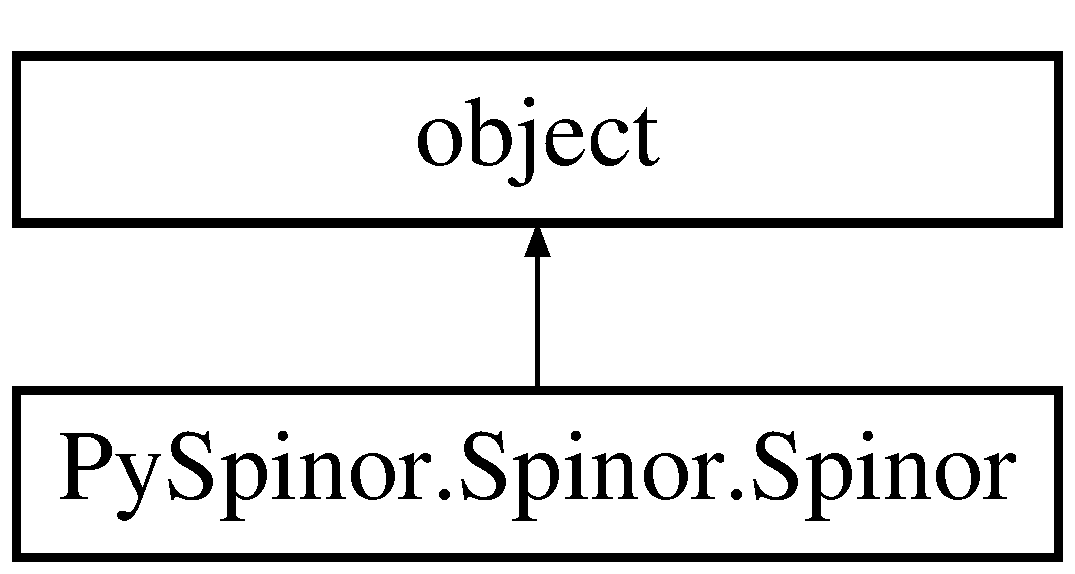
\includegraphics[height=2.000000cm]{class_py_spinor_1_1_spinor_1_1_spinor}
\end{center}
\end{figure}
\subsection*{Classes}
\begin{DoxyCompactItemize}
\item 
class \hyperlink{class_py_spinor_1_1_spinor_1_1_spinor_1_1spinor}{spinor}
\end{DoxyCompactItemize}
\subsection*{Public Member Functions}
\begin{DoxyCompactItemize}
\item 
def \hyperlink{class_py_spinor_1_1_spinor_1_1_spinor_a9b056b1d6a909bc378dfed5375eeb961}{\+\_\+\+\_\+init\+\_\+\+\_\+}
\item 
def \hyperlink{class_py_spinor_1_1_spinor_1_1_spinor_a3bd7138871861b01b8206982230c63ed}{\+\_\+\+\_\+call\+\_\+\+\_\+} (self, polarisation)
\begin{DoxyCompactList}\small\item\em Make the object a functor. \end{DoxyCompactList}\item 
def \hyperlink{class_py_spinor_1_1_spinor_1_1_spinor_ad5401a5668ab41cff0f76cc270ed96d1}{\+\_\+\+\_\+str\+\_\+\+\_\+} (self)
\item 
def \hyperlink{class_py_spinor_1_1_spinor_1_1_spinor_ad48c01a28f221b81c913bf2fbf2cea6d}{\+\_\+\+\_\+ne\+\_\+\+\_\+} (self, other)
\item 
def \hyperlink{class_py_spinor_1_1_spinor_1_1_spinor_ab3bdf966caa2b922ba9ac76952701ee9}{\+\_\+\+\_\+floordiv\+\_\+\+\_\+} (self, other)
\begin{DoxyCompactList}\small\item\em Overload the floor division operator to calculate spinor brackets like \mbox{[}21\mbox{]}. \end{DoxyCompactList}\item 
def \hyperlink{class_py_spinor_1_1_spinor_1_1_spinor_a26eed6b4fd1bfeee0974afbaefd02e40}{\+\_\+\+\_\+pow\+\_\+\+\_\+} (self, other)
\begin{DoxyCompactList}\small\item\em Overload the power operator to calculate spinor brackets like $<$21$>$ \end{DoxyCompactList}\item 
def \hyperlink{class_py_spinor_1_1_spinor_1_1_spinor_ab4a660f4882baa072d3c06845fae9fa7}{get\+Momentum} (self)
\item 
def \hyperlink{class_py_spinor_1_1_spinor_1_1_spinor_a429c47acf609aee5dd41aa580e688de4}{is\+Barred} (self)
\item 
def \hyperlink{class_py_spinor_1_1_spinor_1_1_spinor_abea59fee1e79b530008e25f7e43e737b}{is\+Massless} (self)
\item 
def \hyperlink{class_py_spinor_1_1_spinor_1_1_spinor_ad1202b23d67450b5d097fa5984f4972e}{bar}
\begin{DoxyCompactList}\small\item\em Clever barred calculation which makes the barred spinors look like functors too...but they arent really. \end{DoxyCompactList}\item 
def \hyperlink{class_py_spinor_1_1_spinor_1_1_spinor_a561a2bbb23e5f44bd04a68065da6cced}{dirac\+Eqn} (self)
\end{DoxyCompactItemize}
\subsection*{Public Attributes}
\begin{DoxyCompactItemize}
\item 
\hyperlink{class_py_spinor_1_1_spinor_1_1_spinor_a3a07111900e024ddfacd6b0562d36f11}{I\+D}
\item 
\hyperlink{class_py_spinor_1_1_spinor_1_1_spinor_a0e1deed1ae598a4bda4a648422975cee}{momentum}
\item 
\hyperlink{class_py_spinor_1_1_spinor_1_1_spinor_a40fd29a13815d67b8ee09391440d8781}{barred}
\item 
\hyperlink{class_py_spinor_1_1_spinor_1_1_spinor_a5dbc10a0e243e6b0e5039583fe4dd63f}{fermion}
\item 
\hyperlink{class_py_spinor_1_1_spinor_1_1_spinor_a519f8be747d03caa97141c1d0146cd1c}{mass}
\item 
\hyperlink{class_py_spinor_1_1_spinor_1_1_spinor_ade40e15caea3f801f46629f948e33137}{pols}
\end{DoxyCompactItemize}


\subsection{Detailed Description}
\hyperlink{class_py_spinor_1_1_spinor_1_1_spinor}{Spinor} class Woo! Py\+Spinor! Spinors are defined using contravariant momenta. 

\subsection{Constructor \& Destructor Documentation}
\hypertarget{class_py_spinor_1_1_spinor_1_1_spinor_a9b056b1d6a909bc378dfed5375eeb961}{}\index{Py\+Spinor\+::\+Spinor\+::\+Spinor@{Py\+Spinor\+::\+Spinor\+::\+Spinor}!\+\_\+\+\_\+init\+\_\+\+\_\+@{\+\_\+\+\_\+init\+\_\+\+\_\+}}
\index{\+\_\+\+\_\+init\+\_\+\+\_\+@{\+\_\+\+\_\+init\+\_\+\+\_\+}!Py\+Spinor\+::\+Spinor\+::\+Spinor@{Py\+Spinor\+::\+Spinor\+::\+Spinor}}
\subsubsection[{\+\_\+\+\_\+init\+\_\+\+\_\+}]{\setlength{\rightskip}{0pt plus 5cm}def Py\+Spinor.\+Spinor.\+Spinor.\+\_\+\+\_\+init\+\_\+\+\_\+ (
\begin{DoxyParamCaption}
\item[{}]{self, }
\item[{}]{momentum, }
\item[{}]{barred = {\ttfamily False}, }
\item[{}]{fermion = {\ttfamily True}, }
\item[{}]{I\+D = {\ttfamily None}}
\end{DoxyParamCaption}
)}\label{class_py_spinor_1_1_spinor_1_1_spinor_a9b056b1d6a909bc378dfed5375eeb961}


\subsection{Member Function Documentation}
\hypertarget{class_py_spinor_1_1_spinor_1_1_spinor_a3bd7138871861b01b8206982230c63ed}{}\index{Py\+Spinor\+::\+Spinor\+::\+Spinor@{Py\+Spinor\+::\+Spinor\+::\+Spinor}!\+\_\+\+\_\+call\+\_\+\+\_\+@{\+\_\+\+\_\+call\+\_\+\+\_\+}}
\index{\+\_\+\+\_\+call\+\_\+\+\_\+@{\+\_\+\+\_\+call\+\_\+\+\_\+}!Py\+Spinor\+::\+Spinor\+::\+Spinor@{Py\+Spinor\+::\+Spinor\+::\+Spinor}}
\subsubsection[{\+\_\+\+\_\+call\+\_\+\+\_\+}]{\setlength{\rightskip}{0pt plus 5cm}def Py\+Spinor.\+Spinor.\+Spinor.\+\_\+\+\_\+call\+\_\+\+\_\+ (
\begin{DoxyParamCaption}
\item[{}]{self, }
\item[{}]{polarisation}
\end{DoxyParamCaption}
)}\label{class_py_spinor_1_1_spinor_1_1_spinor_a3bd7138871861b01b8206982230c63ed}


Make the object a functor. 

\hypertarget{class_py_spinor_1_1_spinor_1_1_spinor_ab3bdf966caa2b922ba9ac76952701ee9}{}\index{Py\+Spinor\+::\+Spinor\+::\+Spinor@{Py\+Spinor\+::\+Spinor\+::\+Spinor}!\+\_\+\+\_\+floordiv\+\_\+\+\_\+@{\+\_\+\+\_\+floordiv\+\_\+\+\_\+}}
\index{\+\_\+\+\_\+floordiv\+\_\+\+\_\+@{\+\_\+\+\_\+floordiv\+\_\+\+\_\+}!Py\+Spinor\+::\+Spinor\+::\+Spinor@{Py\+Spinor\+::\+Spinor\+::\+Spinor}}
\subsubsection[{\+\_\+\+\_\+floordiv\+\_\+\+\_\+}]{\setlength{\rightskip}{0pt plus 5cm}def Py\+Spinor.\+Spinor.\+Spinor.\+\_\+\+\_\+floordiv\+\_\+\+\_\+ (
\begin{DoxyParamCaption}
\item[{}]{self, }
\item[{}]{other}
\end{DoxyParamCaption}
)}\label{class_py_spinor_1_1_spinor_1_1_spinor_ab3bdf966caa2b922ba9ac76952701ee9}


Overload the floor division operator to calculate spinor brackets like \mbox{[}21\mbox{]}. 

\hypertarget{class_py_spinor_1_1_spinor_1_1_spinor_ad48c01a28f221b81c913bf2fbf2cea6d}{}\index{Py\+Spinor\+::\+Spinor\+::\+Spinor@{Py\+Spinor\+::\+Spinor\+::\+Spinor}!\+\_\+\+\_\+ne\+\_\+\+\_\+@{\+\_\+\+\_\+ne\+\_\+\+\_\+}}
\index{\+\_\+\+\_\+ne\+\_\+\+\_\+@{\+\_\+\+\_\+ne\+\_\+\+\_\+}!Py\+Spinor\+::\+Spinor\+::\+Spinor@{Py\+Spinor\+::\+Spinor\+::\+Spinor}}
\subsubsection[{\+\_\+\+\_\+ne\+\_\+\+\_\+}]{\setlength{\rightskip}{0pt plus 5cm}def Py\+Spinor.\+Spinor.\+Spinor.\+\_\+\+\_\+ne\+\_\+\+\_\+ (
\begin{DoxyParamCaption}
\item[{}]{self, }
\item[{}]{other}
\end{DoxyParamCaption}
)}\label{class_py_spinor_1_1_spinor_1_1_spinor_ad48c01a28f221b81c913bf2fbf2cea6d}
\hypertarget{class_py_spinor_1_1_spinor_1_1_spinor_a26eed6b4fd1bfeee0974afbaefd02e40}{}\index{Py\+Spinor\+::\+Spinor\+::\+Spinor@{Py\+Spinor\+::\+Spinor\+::\+Spinor}!\+\_\+\+\_\+pow\+\_\+\+\_\+@{\+\_\+\+\_\+pow\+\_\+\+\_\+}}
\index{\+\_\+\+\_\+pow\+\_\+\+\_\+@{\+\_\+\+\_\+pow\+\_\+\+\_\+}!Py\+Spinor\+::\+Spinor\+::\+Spinor@{Py\+Spinor\+::\+Spinor\+::\+Spinor}}
\subsubsection[{\+\_\+\+\_\+pow\+\_\+\+\_\+}]{\setlength{\rightskip}{0pt plus 5cm}def Py\+Spinor.\+Spinor.\+Spinor.\+\_\+\+\_\+pow\+\_\+\+\_\+ (
\begin{DoxyParamCaption}
\item[{}]{self, }
\item[{}]{other}
\end{DoxyParamCaption}
)}\label{class_py_spinor_1_1_spinor_1_1_spinor_a26eed6b4fd1bfeee0974afbaefd02e40}


Overload the power operator to calculate spinor brackets like $<$21$>$ 

\hypertarget{class_py_spinor_1_1_spinor_1_1_spinor_ad5401a5668ab41cff0f76cc270ed96d1}{}\index{Py\+Spinor\+::\+Spinor\+::\+Spinor@{Py\+Spinor\+::\+Spinor\+::\+Spinor}!\+\_\+\+\_\+str\+\_\+\+\_\+@{\+\_\+\+\_\+str\+\_\+\+\_\+}}
\index{\+\_\+\+\_\+str\+\_\+\+\_\+@{\+\_\+\+\_\+str\+\_\+\+\_\+}!Py\+Spinor\+::\+Spinor\+::\+Spinor@{Py\+Spinor\+::\+Spinor\+::\+Spinor}}
\subsubsection[{\+\_\+\+\_\+str\+\_\+\+\_\+}]{\setlength{\rightskip}{0pt plus 5cm}def Py\+Spinor.\+Spinor.\+Spinor.\+\_\+\+\_\+str\+\_\+\+\_\+ (
\begin{DoxyParamCaption}
\item[{}]{self}
\end{DoxyParamCaption}
)}\label{class_py_spinor_1_1_spinor_1_1_spinor_ad5401a5668ab41cff0f76cc270ed96d1}
\hypertarget{class_py_spinor_1_1_spinor_1_1_spinor_ad1202b23d67450b5d097fa5984f4972e}{}\index{Py\+Spinor\+::\+Spinor\+::\+Spinor@{Py\+Spinor\+::\+Spinor\+::\+Spinor}!bar@{bar}}
\index{bar@{bar}!Py\+Spinor\+::\+Spinor\+::\+Spinor@{Py\+Spinor\+::\+Spinor\+::\+Spinor}}
\subsubsection[{bar}]{\setlength{\rightskip}{0pt plus 5cm}def Py\+Spinor.\+Spinor.\+Spinor.\+bar (
\begin{DoxyParamCaption}
\item[{}]{self, }
\item[{}]{pol = {\ttfamily None}}
\end{DoxyParamCaption}
)}\label{class_py_spinor_1_1_spinor_1_1_spinor_ad1202b23d67450b5d097fa5984f4972e}


Clever barred calculation which makes the barred spinors look like functors too...but they arent really. 

\hypertarget{class_py_spinor_1_1_spinor_1_1_spinor_a561a2bbb23e5f44bd04a68065da6cced}{}\index{Py\+Spinor\+::\+Spinor\+::\+Spinor@{Py\+Spinor\+::\+Spinor\+::\+Spinor}!dirac\+Eqn@{dirac\+Eqn}}
\index{dirac\+Eqn@{dirac\+Eqn}!Py\+Spinor\+::\+Spinor\+::\+Spinor@{Py\+Spinor\+::\+Spinor\+::\+Spinor}}
\subsubsection[{dirac\+Eqn}]{\setlength{\rightskip}{0pt plus 5cm}def Py\+Spinor.\+Spinor.\+Spinor.\+dirac\+Eqn (
\begin{DoxyParamCaption}
\item[{}]{self}
\end{DoxyParamCaption}
)}\label{class_py_spinor_1_1_spinor_1_1_spinor_a561a2bbb23e5f44bd04a68065da6cced}
\hypertarget{class_py_spinor_1_1_spinor_1_1_spinor_ab4a660f4882baa072d3c06845fae9fa7}{}\index{Py\+Spinor\+::\+Spinor\+::\+Spinor@{Py\+Spinor\+::\+Spinor\+::\+Spinor}!get\+Momentum@{get\+Momentum}}
\index{get\+Momentum@{get\+Momentum}!Py\+Spinor\+::\+Spinor\+::\+Spinor@{Py\+Spinor\+::\+Spinor\+::\+Spinor}}
\subsubsection[{get\+Momentum}]{\setlength{\rightskip}{0pt plus 5cm}def Py\+Spinor.\+Spinor.\+Spinor.\+get\+Momentum (
\begin{DoxyParamCaption}
\item[{}]{self}
\end{DoxyParamCaption}
)}\label{class_py_spinor_1_1_spinor_1_1_spinor_ab4a660f4882baa072d3c06845fae9fa7}
\hypertarget{class_py_spinor_1_1_spinor_1_1_spinor_a429c47acf609aee5dd41aa580e688de4}{}\index{Py\+Spinor\+::\+Spinor\+::\+Spinor@{Py\+Spinor\+::\+Spinor\+::\+Spinor}!is\+Barred@{is\+Barred}}
\index{is\+Barred@{is\+Barred}!Py\+Spinor\+::\+Spinor\+::\+Spinor@{Py\+Spinor\+::\+Spinor\+::\+Spinor}}
\subsubsection[{is\+Barred}]{\setlength{\rightskip}{0pt plus 5cm}def Py\+Spinor.\+Spinor.\+Spinor.\+is\+Barred (
\begin{DoxyParamCaption}
\item[{}]{self}
\end{DoxyParamCaption}
)}\label{class_py_spinor_1_1_spinor_1_1_spinor_a429c47acf609aee5dd41aa580e688de4}
\hypertarget{class_py_spinor_1_1_spinor_1_1_spinor_abea59fee1e79b530008e25f7e43e737b}{}\index{Py\+Spinor\+::\+Spinor\+::\+Spinor@{Py\+Spinor\+::\+Spinor\+::\+Spinor}!is\+Massless@{is\+Massless}}
\index{is\+Massless@{is\+Massless}!Py\+Spinor\+::\+Spinor\+::\+Spinor@{Py\+Spinor\+::\+Spinor\+::\+Spinor}}
\subsubsection[{is\+Massless}]{\setlength{\rightskip}{0pt plus 5cm}def Py\+Spinor.\+Spinor.\+Spinor.\+is\+Massless (
\begin{DoxyParamCaption}
\item[{}]{self}
\end{DoxyParamCaption}
)}\label{class_py_spinor_1_1_spinor_1_1_spinor_abea59fee1e79b530008e25f7e43e737b}


\subsection{Member Data Documentation}
\hypertarget{class_py_spinor_1_1_spinor_1_1_spinor_a40fd29a13815d67b8ee09391440d8781}{}\index{Py\+Spinor\+::\+Spinor\+::\+Spinor@{Py\+Spinor\+::\+Spinor\+::\+Spinor}!barred@{barred}}
\index{barred@{barred}!Py\+Spinor\+::\+Spinor\+::\+Spinor@{Py\+Spinor\+::\+Spinor\+::\+Spinor}}
\subsubsection[{barred}]{\setlength{\rightskip}{0pt plus 5cm}Py\+Spinor.\+Spinor.\+Spinor.\+barred}\label{class_py_spinor_1_1_spinor_1_1_spinor_a40fd29a13815d67b8ee09391440d8781}
\hypertarget{class_py_spinor_1_1_spinor_1_1_spinor_a5dbc10a0e243e6b0e5039583fe4dd63f}{}\index{Py\+Spinor\+::\+Spinor\+::\+Spinor@{Py\+Spinor\+::\+Spinor\+::\+Spinor}!fermion@{fermion}}
\index{fermion@{fermion}!Py\+Spinor\+::\+Spinor\+::\+Spinor@{Py\+Spinor\+::\+Spinor\+::\+Spinor}}
\subsubsection[{fermion}]{\setlength{\rightskip}{0pt plus 5cm}Py\+Spinor.\+Spinor.\+Spinor.\+fermion}\label{class_py_spinor_1_1_spinor_1_1_spinor_a5dbc10a0e243e6b0e5039583fe4dd63f}
\hypertarget{class_py_spinor_1_1_spinor_1_1_spinor_a3a07111900e024ddfacd6b0562d36f11}{}\index{Py\+Spinor\+::\+Spinor\+::\+Spinor@{Py\+Spinor\+::\+Spinor\+::\+Spinor}!I\+D@{I\+D}}
\index{I\+D@{I\+D}!Py\+Spinor\+::\+Spinor\+::\+Spinor@{Py\+Spinor\+::\+Spinor\+::\+Spinor}}
\subsubsection[{I\+D}]{\setlength{\rightskip}{0pt plus 5cm}Py\+Spinor.\+Spinor.\+Spinor.\+I\+D}\label{class_py_spinor_1_1_spinor_1_1_spinor_a3a07111900e024ddfacd6b0562d36f11}
\hypertarget{class_py_spinor_1_1_spinor_1_1_spinor_a519f8be747d03caa97141c1d0146cd1c}{}\index{Py\+Spinor\+::\+Spinor\+::\+Spinor@{Py\+Spinor\+::\+Spinor\+::\+Spinor}!mass@{mass}}
\index{mass@{mass}!Py\+Spinor\+::\+Spinor\+::\+Spinor@{Py\+Spinor\+::\+Spinor\+::\+Spinor}}
\subsubsection[{mass}]{\setlength{\rightskip}{0pt plus 5cm}Py\+Spinor.\+Spinor.\+Spinor.\+mass}\label{class_py_spinor_1_1_spinor_1_1_spinor_a519f8be747d03caa97141c1d0146cd1c}
\hypertarget{class_py_spinor_1_1_spinor_1_1_spinor_a0e1deed1ae598a4bda4a648422975cee}{}\index{Py\+Spinor\+::\+Spinor\+::\+Spinor@{Py\+Spinor\+::\+Spinor\+::\+Spinor}!momentum@{momentum}}
\index{momentum@{momentum}!Py\+Spinor\+::\+Spinor\+::\+Spinor@{Py\+Spinor\+::\+Spinor\+::\+Spinor}}
\subsubsection[{momentum}]{\setlength{\rightskip}{0pt plus 5cm}Py\+Spinor.\+Spinor.\+Spinor.\+momentum}\label{class_py_spinor_1_1_spinor_1_1_spinor_a0e1deed1ae598a4bda4a648422975cee}
\hypertarget{class_py_spinor_1_1_spinor_1_1_spinor_ade40e15caea3f801f46629f948e33137}{}\index{Py\+Spinor\+::\+Spinor\+::\+Spinor@{Py\+Spinor\+::\+Spinor\+::\+Spinor}!pols@{pols}}
\index{pols@{pols}!Py\+Spinor\+::\+Spinor\+::\+Spinor@{Py\+Spinor\+::\+Spinor\+::\+Spinor}}
\subsubsection[{pols}]{\setlength{\rightskip}{0pt plus 5cm}Py\+Spinor.\+Spinor.\+Spinor.\+pols}\label{class_py_spinor_1_1_spinor_1_1_spinor_ade40e15caea3f801f46629f948e33137}


The documentation for this class was generated from the following file\+:\begin{DoxyCompactItemize}
\item 
Py\+Spinor/\hyperlink{_spinor_8py}{Spinor.\+py}\end{DoxyCompactItemize}

\hypertarget{class_py_spinor_1_1spinor_string_1_1spinor_string}{}\section{Py\+Spinor.\+spinor\+String.\+spinor\+String Class Reference}
\label{class_py_spinor_1_1spinor_string_1_1spinor_string}\index{Py\+Spinor.\+spinor\+String.\+spinor\+String@{Py\+Spinor.\+spinor\+String.\+spinor\+String}}


\hyperlink{namespace_py_spinor_1_1_spinor}{Spinor} string class Depricated?  


Inheritance diagram for Py\+Spinor.\+spinor\+String.\+spinor\+String\+:\begin{figure}[H]
\begin{center}
\leavevmode
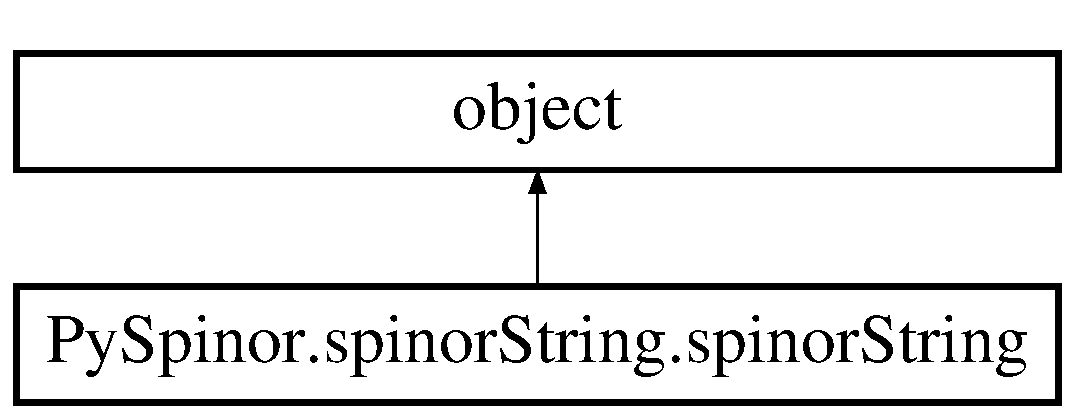
\includegraphics[height=2.000000cm]{class_py_spinor_1_1spinor_string_1_1spinor_string}
\end{center}
\end{figure}
\subsection*{Public Member Functions}
\begin{DoxyCompactItemize}
\item 
def \hyperlink{class_py_spinor_1_1spinor_string_1_1spinor_string_a5e4372ca15f52da36bfa4ac673d857f4}{\+\_\+\+\_\+init\+\_\+\+\_\+} (self, args, kwargs)
\item 
def \hyperlink{class_py_spinor_1_1spinor_string_1_1spinor_string_acaf7fd9a4f3cb88968f4dccfad0939d8}{clear\+String} (self)
\item 
def \hyperlink{class_py_spinor_1_1spinor_string_1_1spinor_string_a2758ca6f8d4970e6dffbc7a882f8e999}{add\+String} (self)
\item 
def \hyperlink{class_py_spinor_1_1spinor_string_1_1spinor_string_abb012d0d474023b69d3fcbc75da92507}{get\+La\+Te\+X} (self, \hyperlink{class_py_spinor_1_1spinor_string_1_1spinor_string_aa965cbe6144646c9ec83c663a29f1eef}{file\+Name})
\item 
def \hyperlink{class_py_spinor_1_1spinor_string_1_1spinor_string_a45825ae590114faf0f86cffd1d06af8b}{compile\+La\+Te\+X} (self)
\end{DoxyCompactItemize}
\subsection*{Public Attributes}
\begin{DoxyCompactItemize}
\item 
\hyperlink{class_py_spinor_1_1spinor_string_1_1spinor_string_a891469ad4c3d0d8bbfa639b9ff1bbb59}{output}
\item 
\hyperlink{class_py_spinor_1_1spinor_string_1_1spinor_string_a3f8abb6e2d071f76f0f6260fb9184351}{S\+U3}
\item 
\hyperlink{class_py_spinor_1_1spinor_string_1_1spinor_string_ae5dd6375cdb42c8abba14c9a06475ab9}{String}
\item 
\hyperlink{class_py_spinor_1_1spinor_string_1_1spinor_string_a71864ffaa13f3d5a408d0a0b2cbbc6a4}{prefactor}
\item 
\hyperlink{class_py_spinor_1_1spinor_string_1_1spinor_string_a274c6711b690c9edd840b31f89109694}{colour}
\item 
\hyperlink{class_py_spinor_1_1spinor_string_1_1spinor_string_aa965cbe6144646c9ec83c663a29f1eef}{file\+Name}
\end{DoxyCompactItemize}


\subsection{Detailed Description}
\hyperlink{namespace_py_spinor_1_1_spinor}{Spinor} string class Depricated? 

\subsection{Constructor \& Destructor Documentation}
\hypertarget{class_py_spinor_1_1spinor_string_1_1spinor_string_a5e4372ca15f52da36bfa4ac673d857f4}{}\index{Py\+Spinor\+::spinor\+String\+::spinor\+String@{Py\+Spinor\+::spinor\+String\+::spinor\+String}!\+\_\+\+\_\+init\+\_\+\+\_\+@{\+\_\+\+\_\+init\+\_\+\+\_\+}}
\index{\+\_\+\+\_\+init\+\_\+\+\_\+@{\+\_\+\+\_\+init\+\_\+\+\_\+}!Py\+Spinor\+::spinor\+String\+::spinor\+String@{Py\+Spinor\+::spinor\+String\+::spinor\+String}}
\subsubsection[{\+\_\+\+\_\+init\+\_\+\+\_\+}]{\setlength{\rightskip}{0pt plus 5cm}def Py\+Spinor.\+spinor\+String.\+spinor\+String.\+\_\+\+\_\+init\+\_\+\+\_\+ (
\begin{DoxyParamCaption}
\item[{}]{self, }
\item[{}]{args, }
\item[{}]{kwargs}
\end{DoxyParamCaption}
)}\label{class_py_spinor_1_1spinor_string_1_1spinor_string_a5e4372ca15f52da36bfa4ac673d857f4}


\subsection{Member Function Documentation}
\hypertarget{class_py_spinor_1_1spinor_string_1_1spinor_string_a2758ca6f8d4970e6dffbc7a882f8e999}{}\index{Py\+Spinor\+::spinor\+String\+::spinor\+String@{Py\+Spinor\+::spinor\+String\+::spinor\+String}!add\+String@{add\+String}}
\index{add\+String@{add\+String}!Py\+Spinor\+::spinor\+String\+::spinor\+String@{Py\+Spinor\+::spinor\+String\+::spinor\+String}}
\subsubsection[{add\+String}]{\setlength{\rightskip}{0pt plus 5cm}def Py\+Spinor.\+spinor\+String.\+spinor\+String.\+add\+String (
\begin{DoxyParamCaption}
\item[{}]{self}
\end{DoxyParamCaption}
)}\label{class_py_spinor_1_1spinor_string_1_1spinor_string_a2758ca6f8d4970e6dffbc7a882f8e999}
\hypertarget{class_py_spinor_1_1spinor_string_1_1spinor_string_acaf7fd9a4f3cb88968f4dccfad0939d8}{}\index{Py\+Spinor\+::spinor\+String\+::spinor\+String@{Py\+Spinor\+::spinor\+String\+::spinor\+String}!clear\+String@{clear\+String}}
\index{clear\+String@{clear\+String}!Py\+Spinor\+::spinor\+String\+::spinor\+String@{Py\+Spinor\+::spinor\+String\+::spinor\+String}}
\subsubsection[{clear\+String}]{\setlength{\rightskip}{0pt plus 5cm}def Py\+Spinor.\+spinor\+String.\+spinor\+String.\+clear\+String (
\begin{DoxyParamCaption}
\item[{}]{self}
\end{DoxyParamCaption}
)}\label{class_py_spinor_1_1spinor_string_1_1spinor_string_acaf7fd9a4f3cb88968f4dccfad0939d8}
\hypertarget{class_py_spinor_1_1spinor_string_1_1spinor_string_a45825ae590114faf0f86cffd1d06af8b}{}\index{Py\+Spinor\+::spinor\+String\+::spinor\+String@{Py\+Spinor\+::spinor\+String\+::spinor\+String}!compile\+La\+Te\+X@{compile\+La\+Te\+X}}
\index{compile\+La\+Te\+X@{compile\+La\+Te\+X}!Py\+Spinor\+::spinor\+String\+::spinor\+String@{Py\+Spinor\+::spinor\+String\+::spinor\+String}}
\subsubsection[{compile\+La\+Te\+X}]{\setlength{\rightskip}{0pt plus 5cm}def Py\+Spinor.\+spinor\+String.\+spinor\+String.\+compile\+La\+Te\+X (
\begin{DoxyParamCaption}
\item[{}]{self}
\end{DoxyParamCaption}
)}\label{class_py_spinor_1_1spinor_string_1_1spinor_string_a45825ae590114faf0f86cffd1d06af8b}
\hypertarget{class_py_spinor_1_1spinor_string_1_1spinor_string_abb012d0d474023b69d3fcbc75da92507}{}\index{Py\+Spinor\+::spinor\+String\+::spinor\+String@{Py\+Spinor\+::spinor\+String\+::spinor\+String}!get\+La\+Te\+X@{get\+La\+Te\+X}}
\index{get\+La\+Te\+X@{get\+La\+Te\+X}!Py\+Spinor\+::spinor\+String\+::spinor\+String@{Py\+Spinor\+::spinor\+String\+::spinor\+String}}
\subsubsection[{get\+La\+Te\+X}]{\setlength{\rightskip}{0pt plus 5cm}def Py\+Spinor.\+spinor\+String.\+spinor\+String.\+get\+La\+Te\+X (
\begin{DoxyParamCaption}
\item[{}]{self, }
\item[{}]{file\+Name}
\end{DoxyParamCaption}
)}\label{class_py_spinor_1_1spinor_string_1_1spinor_string_abb012d0d474023b69d3fcbc75da92507}


\subsection{Member Data Documentation}
\hypertarget{class_py_spinor_1_1spinor_string_1_1spinor_string_a274c6711b690c9edd840b31f89109694}{}\index{Py\+Spinor\+::spinor\+String\+::spinor\+String@{Py\+Spinor\+::spinor\+String\+::spinor\+String}!colour@{colour}}
\index{colour@{colour}!Py\+Spinor\+::spinor\+String\+::spinor\+String@{Py\+Spinor\+::spinor\+String\+::spinor\+String}}
\subsubsection[{colour}]{\setlength{\rightskip}{0pt plus 5cm}Py\+Spinor.\+spinor\+String.\+spinor\+String.\+colour}\label{class_py_spinor_1_1spinor_string_1_1spinor_string_a274c6711b690c9edd840b31f89109694}
\hypertarget{class_py_spinor_1_1spinor_string_1_1spinor_string_aa965cbe6144646c9ec83c663a29f1eef}{}\index{Py\+Spinor\+::spinor\+String\+::spinor\+String@{Py\+Spinor\+::spinor\+String\+::spinor\+String}!file\+Name@{file\+Name}}
\index{file\+Name@{file\+Name}!Py\+Spinor\+::spinor\+String\+::spinor\+String@{Py\+Spinor\+::spinor\+String\+::spinor\+String}}
\subsubsection[{file\+Name}]{\setlength{\rightskip}{0pt plus 5cm}Py\+Spinor.\+spinor\+String.\+spinor\+String.\+file\+Name}\label{class_py_spinor_1_1spinor_string_1_1spinor_string_aa965cbe6144646c9ec83c663a29f1eef}
\hypertarget{class_py_spinor_1_1spinor_string_1_1spinor_string_a891469ad4c3d0d8bbfa639b9ff1bbb59}{}\index{Py\+Spinor\+::spinor\+String\+::spinor\+String@{Py\+Spinor\+::spinor\+String\+::spinor\+String}!output@{output}}
\index{output@{output}!Py\+Spinor\+::spinor\+String\+::spinor\+String@{Py\+Spinor\+::spinor\+String\+::spinor\+String}}
\subsubsection[{output}]{\setlength{\rightskip}{0pt plus 5cm}Py\+Spinor.\+spinor\+String.\+spinor\+String.\+output}\label{class_py_spinor_1_1spinor_string_1_1spinor_string_a891469ad4c3d0d8bbfa639b9ff1bbb59}
\hypertarget{class_py_spinor_1_1spinor_string_1_1spinor_string_a71864ffaa13f3d5a408d0a0b2cbbc6a4}{}\index{Py\+Spinor\+::spinor\+String\+::spinor\+String@{Py\+Spinor\+::spinor\+String\+::spinor\+String}!prefactor@{prefactor}}
\index{prefactor@{prefactor}!Py\+Spinor\+::spinor\+String\+::spinor\+String@{Py\+Spinor\+::spinor\+String\+::spinor\+String}}
\subsubsection[{prefactor}]{\setlength{\rightskip}{0pt plus 5cm}Py\+Spinor.\+spinor\+String.\+spinor\+String.\+prefactor}\label{class_py_spinor_1_1spinor_string_1_1spinor_string_a71864ffaa13f3d5a408d0a0b2cbbc6a4}
\hypertarget{class_py_spinor_1_1spinor_string_1_1spinor_string_ae5dd6375cdb42c8abba14c9a06475ab9}{}\index{Py\+Spinor\+::spinor\+String\+::spinor\+String@{Py\+Spinor\+::spinor\+String\+::spinor\+String}!String@{String}}
\index{String@{String}!Py\+Spinor\+::spinor\+String\+::spinor\+String@{Py\+Spinor\+::spinor\+String\+::spinor\+String}}
\subsubsection[{String}]{\setlength{\rightskip}{0pt plus 5cm}Py\+Spinor.\+spinor\+String.\+spinor\+String.\+String}\label{class_py_spinor_1_1spinor_string_1_1spinor_string_ae5dd6375cdb42c8abba14c9a06475ab9}
\hypertarget{class_py_spinor_1_1spinor_string_1_1spinor_string_a3f8abb6e2d071f76f0f6260fb9184351}{}\index{Py\+Spinor\+::spinor\+String\+::spinor\+String@{Py\+Spinor\+::spinor\+String\+::spinor\+String}!S\+U3@{S\+U3}}
\index{S\+U3@{S\+U3}!Py\+Spinor\+::spinor\+String\+::spinor\+String@{Py\+Spinor\+::spinor\+String\+::spinor\+String}}
\subsubsection[{S\+U3}]{\setlength{\rightskip}{0pt plus 5cm}Py\+Spinor.\+spinor\+String.\+spinor\+String.\+S\+U3}\label{class_py_spinor_1_1spinor_string_1_1spinor_string_a3f8abb6e2d071f76f0f6260fb9184351}


The documentation for this class was generated from the following file\+:\begin{DoxyCompactItemize}
\item 
Py\+Spinor/\hyperlink{spinor_string_8py}{spinor\+String.\+py}\end{DoxyCompactItemize}

\hypertarget{class_py_spinor_1_1_spinor_tensor_1_1_spinor_tensor}{}\section{Py\+Spinor.\+Spinor\+Tensor.\+Spinor\+Tensor Class Reference}
\label{class_py_spinor_1_1_spinor_tensor_1_1_spinor_tensor}\index{Py\+Spinor.\+Spinor\+Tensor.\+Spinor\+Tensor@{Py\+Spinor.\+Spinor\+Tensor.\+Spinor\+Tensor}}


\hyperlink{namespace_py_spinor_1_1_tensor}{Tensor} with spinors as appearing in specific applications Will need rewrite post \hyperlink{namespace_py_spinor_1_1_tensor}{Tensor} update.  


Inheritance diagram for Py\+Spinor.\+Spinor\+Tensor.\+Spinor\+Tensor\+:\begin{figure}[H]
\begin{center}
\leavevmode
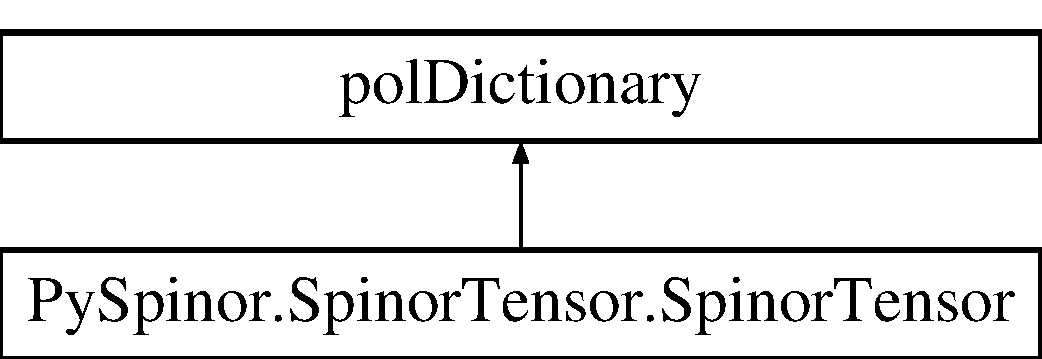
\includegraphics[height=2.000000cm]{class_py_spinor_1_1_spinor_tensor_1_1_spinor_tensor}
\end{center}
\end{figure}
\subsection*{Classes}
\begin{DoxyCompactItemize}
\item 
class \hyperlink{class_py_spinor_1_1_spinor_tensor_1_1_spinor_tensor_1_1tensor}{tensor}
\end{DoxyCompactItemize}
\subsection*{Public Member Functions}
\begin{DoxyCompactItemize}
\item 
def \hyperlink{class_py_spinor_1_1_spinor_tensor_1_1_spinor_tensor_ad1bfc424fc8b77321c2d0514c5645423}{\+\_\+\+\_\+init\+\_\+\+\_\+}
\item 
def \hyperlink{class_py_spinor_1_1_spinor_tensor_1_1_spinor_tensor_a7f52ba9bc232e7274e5d2440fec9b4fb}{contract} (self, other1, other2)
\begin{DoxyCompactList}\small\item\em Contraction for the full \hyperlink{namespace_py_spinor_1_1pol_dictionary}{pol\+Dictionary} \hyperlink{namespace_py_spinor_1_1_tensor}{Tensor} object. \end{DoxyCompactList}\end{DoxyCompactItemize}
\subsection*{Public Attributes}
\begin{DoxyCompactItemize}
\item 
\hyperlink{class_py_spinor_1_1_spinor_tensor_1_1_spinor_tensor_ac758bf30544b7f155fec43057a87df83}{spin1}
\item 
\hyperlink{class_py_spinor_1_1_spinor_tensor_1_1_spinor_tensor_a9d26b8b1a6971bb1529817fa1a93b10c}{spin2}
\item 
\hyperlink{class_py_spinor_1_1_spinor_tensor_1_1_spinor_tensor_ae258d4d0282e027e8585220aaaa477e2}{index1}
\item 
\hyperlink{class_py_spinor_1_1_spinor_tensor_1_1_spinor_tensor_af96dc3871eedd2d62f26f31188fba05a}{index2}
\item 
\hyperlink{class_py_spinor_1_1_spinor_tensor_1_1_spinor_tensor_a3a080c0f125b49a6bff5225fabbf7139}{upper1}
\item 
\hyperlink{class_py_spinor_1_1_spinor_tensor_1_1_spinor_tensor_a50ca2a0d08e4a54d50ed76a5d0ab3e95}{upper2}
\item 
\hyperlink{class_py_spinor_1_1_spinor_tensor_1_1_spinor_tensor_af75ee8d08e8afa5b1449a945adc6496f}{polarisations}
\end{DoxyCompactItemize}


\subsection{Detailed Description}
\hyperlink{namespace_py_spinor_1_1_tensor}{Tensor} with spinors as appearing in specific applications Will need rewrite post \hyperlink{namespace_py_spinor_1_1_tensor}{Tensor} update. 

\subsection{Constructor \& Destructor Documentation}
\hypertarget{class_py_spinor_1_1_spinor_tensor_1_1_spinor_tensor_ad1bfc424fc8b77321c2d0514c5645423}{}\index{Py\+Spinor\+::\+Spinor\+Tensor\+::\+Spinor\+Tensor@{Py\+Spinor\+::\+Spinor\+Tensor\+::\+Spinor\+Tensor}!\+\_\+\+\_\+init\+\_\+\+\_\+@{\+\_\+\+\_\+init\+\_\+\+\_\+}}
\index{\+\_\+\+\_\+init\+\_\+\+\_\+@{\+\_\+\+\_\+init\+\_\+\+\_\+}!Py\+Spinor\+::\+Spinor\+Tensor\+::\+Spinor\+Tensor@{Py\+Spinor\+::\+Spinor\+Tensor\+::\+Spinor\+Tensor}}
\subsubsection[{\+\_\+\+\_\+init\+\_\+\+\_\+}]{\setlength{\rightskip}{0pt plus 5cm}def Py\+Spinor.\+Spinor\+Tensor.\+Spinor\+Tensor.\+\_\+\+\_\+init\+\_\+\+\_\+ (
\begin{DoxyParamCaption}
\item[{}]{self, }
\item[{}]{spin1, }
\item[{}]{index1, }
\item[{}]{index2, }
\item[{}]{spin2, }
\item[{}]{upper1 = {\ttfamily True}, }
\item[{}]{upper2 = {\ttfamily True}}
\end{DoxyParamCaption}
)}\label{class_py_spinor_1_1_spinor_tensor_1_1_spinor_tensor_ad1bfc424fc8b77321c2d0514c5645423}


\subsection{Member Function Documentation}
\hypertarget{class_py_spinor_1_1_spinor_tensor_1_1_spinor_tensor_a7f52ba9bc232e7274e5d2440fec9b4fb}{}\index{Py\+Spinor\+::\+Spinor\+Tensor\+::\+Spinor\+Tensor@{Py\+Spinor\+::\+Spinor\+Tensor\+::\+Spinor\+Tensor}!contract@{contract}}
\index{contract@{contract}!Py\+Spinor\+::\+Spinor\+Tensor\+::\+Spinor\+Tensor@{Py\+Spinor\+::\+Spinor\+Tensor\+::\+Spinor\+Tensor}}
\subsubsection[{contract}]{\setlength{\rightskip}{0pt plus 5cm}def Py\+Spinor.\+Spinor\+Tensor.\+Spinor\+Tensor.\+contract (
\begin{DoxyParamCaption}
\item[{}]{self, }
\item[{}]{other1, }
\item[{}]{other2}
\end{DoxyParamCaption}
)}\label{class_py_spinor_1_1_spinor_tensor_1_1_spinor_tensor_a7f52ba9bc232e7274e5d2440fec9b4fb}


Contraction for the full \hyperlink{namespace_py_spinor_1_1pol_dictionary}{pol\+Dictionary} \hyperlink{namespace_py_spinor_1_1_tensor}{Tensor} object. 



\subsection{Member Data Documentation}
\hypertarget{class_py_spinor_1_1_spinor_tensor_1_1_spinor_tensor_ae258d4d0282e027e8585220aaaa477e2}{}\index{Py\+Spinor\+::\+Spinor\+Tensor\+::\+Spinor\+Tensor@{Py\+Spinor\+::\+Spinor\+Tensor\+::\+Spinor\+Tensor}!index1@{index1}}
\index{index1@{index1}!Py\+Spinor\+::\+Spinor\+Tensor\+::\+Spinor\+Tensor@{Py\+Spinor\+::\+Spinor\+Tensor\+::\+Spinor\+Tensor}}
\subsubsection[{index1}]{\setlength{\rightskip}{0pt plus 5cm}Py\+Spinor.\+Spinor\+Tensor.\+Spinor\+Tensor.\+index1}\label{class_py_spinor_1_1_spinor_tensor_1_1_spinor_tensor_ae258d4d0282e027e8585220aaaa477e2}
\hypertarget{class_py_spinor_1_1_spinor_tensor_1_1_spinor_tensor_af96dc3871eedd2d62f26f31188fba05a}{}\index{Py\+Spinor\+::\+Spinor\+Tensor\+::\+Spinor\+Tensor@{Py\+Spinor\+::\+Spinor\+Tensor\+::\+Spinor\+Tensor}!index2@{index2}}
\index{index2@{index2}!Py\+Spinor\+::\+Spinor\+Tensor\+::\+Spinor\+Tensor@{Py\+Spinor\+::\+Spinor\+Tensor\+::\+Spinor\+Tensor}}
\subsubsection[{index2}]{\setlength{\rightskip}{0pt plus 5cm}Py\+Spinor.\+Spinor\+Tensor.\+Spinor\+Tensor.\+index2}\label{class_py_spinor_1_1_spinor_tensor_1_1_spinor_tensor_af96dc3871eedd2d62f26f31188fba05a}
\hypertarget{class_py_spinor_1_1_spinor_tensor_1_1_spinor_tensor_af75ee8d08e8afa5b1449a945adc6496f}{}\index{Py\+Spinor\+::\+Spinor\+Tensor\+::\+Spinor\+Tensor@{Py\+Spinor\+::\+Spinor\+Tensor\+::\+Spinor\+Tensor}!polarisations@{polarisations}}
\index{polarisations@{polarisations}!Py\+Spinor\+::\+Spinor\+Tensor\+::\+Spinor\+Tensor@{Py\+Spinor\+::\+Spinor\+Tensor\+::\+Spinor\+Tensor}}
\subsubsection[{polarisations}]{\setlength{\rightskip}{0pt plus 5cm}Py\+Spinor.\+Spinor\+Tensor.\+Spinor\+Tensor.\+polarisations}\label{class_py_spinor_1_1_spinor_tensor_1_1_spinor_tensor_af75ee8d08e8afa5b1449a945adc6496f}
\hypertarget{class_py_spinor_1_1_spinor_tensor_1_1_spinor_tensor_ac758bf30544b7f155fec43057a87df83}{}\index{Py\+Spinor\+::\+Spinor\+Tensor\+::\+Spinor\+Tensor@{Py\+Spinor\+::\+Spinor\+Tensor\+::\+Spinor\+Tensor}!spin1@{spin1}}
\index{spin1@{spin1}!Py\+Spinor\+::\+Spinor\+Tensor\+::\+Spinor\+Tensor@{Py\+Spinor\+::\+Spinor\+Tensor\+::\+Spinor\+Tensor}}
\subsubsection[{spin1}]{\setlength{\rightskip}{0pt plus 5cm}Py\+Spinor.\+Spinor\+Tensor.\+Spinor\+Tensor.\+spin1}\label{class_py_spinor_1_1_spinor_tensor_1_1_spinor_tensor_ac758bf30544b7f155fec43057a87df83}
\hypertarget{class_py_spinor_1_1_spinor_tensor_1_1_spinor_tensor_a9d26b8b1a6971bb1529817fa1a93b10c}{}\index{Py\+Spinor\+::\+Spinor\+Tensor\+::\+Spinor\+Tensor@{Py\+Spinor\+::\+Spinor\+Tensor\+::\+Spinor\+Tensor}!spin2@{spin2}}
\index{spin2@{spin2}!Py\+Spinor\+::\+Spinor\+Tensor\+::\+Spinor\+Tensor@{Py\+Spinor\+::\+Spinor\+Tensor\+::\+Spinor\+Tensor}}
\subsubsection[{spin2}]{\setlength{\rightskip}{0pt plus 5cm}Py\+Spinor.\+Spinor\+Tensor.\+Spinor\+Tensor.\+spin2}\label{class_py_spinor_1_1_spinor_tensor_1_1_spinor_tensor_a9d26b8b1a6971bb1529817fa1a93b10c}
\hypertarget{class_py_spinor_1_1_spinor_tensor_1_1_spinor_tensor_a3a080c0f125b49a6bff5225fabbf7139}{}\index{Py\+Spinor\+::\+Spinor\+Tensor\+::\+Spinor\+Tensor@{Py\+Spinor\+::\+Spinor\+Tensor\+::\+Spinor\+Tensor}!upper1@{upper1}}
\index{upper1@{upper1}!Py\+Spinor\+::\+Spinor\+Tensor\+::\+Spinor\+Tensor@{Py\+Spinor\+::\+Spinor\+Tensor\+::\+Spinor\+Tensor}}
\subsubsection[{upper1}]{\setlength{\rightskip}{0pt plus 5cm}Py\+Spinor.\+Spinor\+Tensor.\+Spinor\+Tensor.\+upper1}\label{class_py_spinor_1_1_spinor_tensor_1_1_spinor_tensor_a3a080c0f125b49a6bff5225fabbf7139}
\hypertarget{class_py_spinor_1_1_spinor_tensor_1_1_spinor_tensor_a50ca2a0d08e4a54d50ed76a5d0ab3e95}{}\index{Py\+Spinor\+::\+Spinor\+Tensor\+::\+Spinor\+Tensor@{Py\+Spinor\+::\+Spinor\+Tensor\+::\+Spinor\+Tensor}!upper2@{upper2}}
\index{upper2@{upper2}!Py\+Spinor\+::\+Spinor\+Tensor\+::\+Spinor\+Tensor@{Py\+Spinor\+::\+Spinor\+Tensor\+::\+Spinor\+Tensor}}
\subsubsection[{upper2}]{\setlength{\rightskip}{0pt plus 5cm}Py\+Spinor.\+Spinor\+Tensor.\+Spinor\+Tensor.\+upper2}\label{class_py_spinor_1_1_spinor_tensor_1_1_spinor_tensor_a50ca2a0d08e4a54d50ed76a5d0ab3e95}


The documentation for this class was generated from the following file\+:\begin{DoxyCompactItemize}
\item 
Py\+Spinor/\hyperlink{_spinor_tensor_8py}{Spinor\+Tensor.\+py}\end{DoxyCompactItemize}

\hypertarget{class_py_spinor_1_1_tensor_1_1_tensor}{}\section{Py\+Spinor.\+Tensor.\+Tensor Class Reference}
\label{class_py_spinor_1_1_tensor_1_1_tensor}\index{Py\+Spinor.\+Tensor.\+Tensor@{Py\+Spinor.\+Tensor.\+Tensor}}


General tensor class.  


Inheritance diagram for Py\+Spinor.\+Tensor.\+Tensor\+:\begin{figure}[H]
\begin{center}
\leavevmode
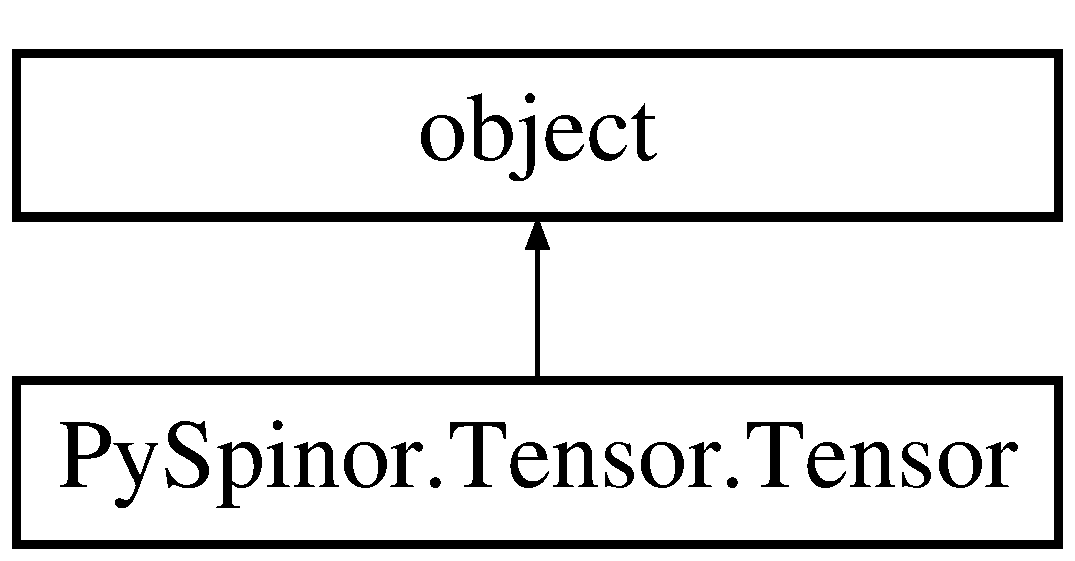
\includegraphics[height=2.000000cm]{class_py_spinor_1_1_tensor_1_1_tensor}
\end{center}
\end{figure}
\subsection*{Public Member Functions}
\begin{DoxyCompactItemize}
\item 
def \hyperlink{class_py_spinor_1_1_tensor_1_1_tensor_a58442b72d740de25daf5e088909f2b5c}{\+\_\+\+\_\+init\+\_\+\+\_\+} (self, mat, i\+List, ul\+List)
\begin{DoxyCompactList}\small\item\em \hyperlink{class_py_spinor_1_1_tensor_1_1_tensor}{Tensor} contructor. \end{DoxyCompactList}\item 
def \hyperlink{class_py_spinor_1_1_tensor_1_1_tensor_ac05df443fff49c9d1829ed85a9e2a322}{\+\_\+\+\_\+str\+\_\+\+\_\+} (self)
\begin{DoxyCompactList}\small\item\em At present, printing a tensor prints only its element array. \end{DoxyCompactList}\item 
def \hyperlink{class_py_spinor_1_1_tensor_1_1_tensor_afe6e90540db57018f6a4d2b2c996f7eb}{\+\_\+\+\_\+add\+\_\+\+\_\+} (self, other)
\begin{DoxyCompactList}\small\item\em Overloading addition for tensors of equal rank, indices and upper/lower lists. \end{DoxyCompactList}\item 
def \hyperlink{class_py_spinor_1_1_tensor_1_1_tensor_a3ff6a865cd53e5d7a2b075da1cadcef4}{\+\_\+\+\_\+sub\+\_\+\+\_\+} (self, other)
\begin{DoxyCompactList}\small\item\em Overloading subtraction for tensors of equal rank, indices and upper/lower lists. \end{DoxyCompactList}\item 
def \hyperlink{class_py_spinor_1_1_tensor_1_1_tensor_a66e613f568c510d30dbd85676984ebf5}{\+\_\+\+\_\+neg\+\_\+\+\_\+} (self)
\begin{DoxyCompactList}\small\item\em Definining negation of tensor elements. \end{DoxyCompactList}\item 
def \hyperlink{class_py_spinor_1_1_tensor_1_1_tensor_a4015087def592e448dd5d27360746220}{\+\_\+\+\_\+div\+\_\+\+\_\+} (self, other)
\begin{DoxyCompactList}\small\item\em Defining division by scalars. \end{DoxyCompactList}\item 
def \hyperlink{class_py_spinor_1_1_tensor_1_1_tensor_afda6832e82410d0e34e9fbe87d421975}{Lower\+Index} (self, indx)
\begin{DoxyCompactList}\small\item\em Lowers (in the Minkowski space sense) the index specified by the string indx. \end{DoxyCompactList}\item 
def \hyperlink{class_py_spinor_1_1_tensor_1_1_tensor_a08ca3ade5041ba809ecc8021e65fc540}{Raise\+Index} (self, indx)
\begin{DoxyCompactList}\small\item\em Raises (in the Minkowski space sense) the index specified by the string indx. \end{DoxyCompactList}\item 
def \hyperlink{class_py_spinor_1_1_tensor_1_1_tensor_a9a632076f7b5fc8503278c61b797e97e}{\+\_\+\+\_\+mul\+\_\+\+\_\+} (self, other)
\begin{DoxyCompactList}\small\item\em Overloading multiplication to take care of contractions/tensor products Also handles tensor-\/scalar multiplication (along with {\bfseries rmul} for scalar-\/tensor) \end{DoxyCompactList}\item 
def \hyperlink{class_py_spinor_1_1_tensor_1_1_tensor_a4faf9399322872bc10fbd763bf3fecf8}{\+\_\+\+\_\+rmul\+\_\+\+\_\+} (self, other)
\begin{DoxyCompactList}\small\item\em Defines scalar-\/tensor multiplication. \end{DoxyCompactList}\item 
def \hyperlink{class_py_spinor_1_1_tensor_1_1_tensor_a38778134828ac330a8fd47db7adecd41}{Get\+Elements} (self)
\begin{DoxyCompactList}\small\item\em Returns a list of all tensor elements. \end{DoxyCompactList}\item 
def \hyperlink{class_py_spinor_1_1_tensor_1_1_tensor_aea7739cc1baad06bca6a8ab7ba3cc95c}{Get\+Indices} (self)
\begin{DoxyCompactList}\small\item\em Returns full list of indices. \end{DoxyCompactList}\item 
def \hyperlink{class_py_spinor_1_1_tensor_1_1_tensor_a5db7ef36bb183c503a300ae40c22a55c}{Get\+Upper\+Lower\+List} (self)
\begin{DoxyCompactList}\small\item\em Returns the list of contra/co-\/ variant states of each index. \end{DoxyCompactList}\item 
def \hyperlink{class_py_spinor_1_1_tensor_1_1_tensor_a1d741384d227a9eeec15ba61685fa436}{Get\+Upper\+Lower\+Dict} (self)
\begin{DoxyCompactList}\small\item\em Returns the dictionary of contra/co-\/ variant states of each index. \end{DoxyCompactList}\item 
def \hyperlink{class_py_spinor_1_1_tensor_1_1_tensor_aeb9b9d580cc278d3d82c3ae6e170e162}{Get\+Element} (self, li)
\begin{DoxyCompactList}\small\item\em Returns particular element of tensor specified by list of ints specifying position. \end{DoxyCompactList}\item 
def \hyperlink{class_py_spinor_1_1_tensor_1_1_tensor_ad3a6e9e20ed888185d1d7a694dcc3656}{Set\+Elements} (self, mat)
\begin{DoxyCompactList}\small\item\em Set elements of tensor by supplying numpy array. \end{DoxyCompactList}\item 
def \hyperlink{class_py_spinor_1_1_tensor_1_1_tensor_a56f26c888dd2c432bbdd90393efc7387}{Set\+Element} (self, pos, val)
\begin{DoxyCompactList}\small\item\em Set single element of tensor by specifying position to be set and value. \end{DoxyCompactList}\item 
def \hyperlink{class_py_spinor_1_1_tensor_1_1_tensor_ac54f08172b7bd55dd4d072089bed4128}{Set\+Indices} (self, i\+List)
\begin{DoxyCompactList}\small\item\em Replaces tensor\textquotesingle{}s index list with i\+List. \end{DoxyCompactList}\item 
def \hyperlink{class_py_spinor_1_1_tensor_1_1_tensor_adb159fcd1553f03294fb0e50896b70cb}{Set\+Upper\+Lower\+List} (self, ul\+List)
\begin{DoxyCompactList}\small\item\em Replaces tensor\textquotesingle{}s upper/lower list with upper/lower list. \end{DoxyCompactList}\item 
def \hyperlink{class_py_spinor_1_1_tensor_1_1_tensor_ac895b7ec88503743bfa53d083c2d79e0}{transpose} (self)
\begin{DoxyCompactList}\small\item\em Defining a transpose (reversing order of all indices) which we may want to restrict to only rank 2 tensors. \end{DoxyCompactList}\end{DoxyCompactItemize}
\subsection*{Public Attributes}
\begin{DoxyCompactItemize}
\item 
\hyperlink{class_py_spinor_1_1_tensor_1_1_tensor_ada0b84b1edfe3b3426c870fa8e7cfe2c}{tensor\+Elements}
\item 
\hyperlink{class_py_spinor_1_1_tensor_1_1_tensor_a3bcb9987ffbcf0a3674960fd0b7581bf}{index\+List}
\item 
\hyperlink{class_py_spinor_1_1_tensor_1_1_tensor_a4ec7810efac6ce40cd7b44c78446ba5a}{upperlower\+List}
\item 
\hyperlink{class_py_spinor_1_1_tensor_1_1_tensor_af112f0319ea0f98158ed9fe744883193}{rank}
\item 
\hyperlink{class_py_spinor_1_1_tensor_1_1_tensor_aa9242fc2995ce134649f8ae71a21cd13}{upperlower\+Dict}
\item 
\hyperlink{class_py_spinor_1_1_tensor_1_1_tensor_aa8cb1d63adaf4edd0924c6eb57e3854f}{Get\+Upper\+Lower\+Dict}
\end{DoxyCompactItemize}


\subsection{Detailed Description}
General tensor class. 

General tensor containing an n-\/dim numpy array for an n-\/rank tensor with a n-\/length list of indices which can be \char`\"{}upper\char`\"{} or \char`\"{}lower\char`\"{} (contra-\/ or covariant, resp.) 

\subsection{Constructor \& Destructor Documentation}
\hypertarget{class_py_spinor_1_1_tensor_1_1_tensor_a58442b72d740de25daf5e088909f2b5c}{}\index{Py\+Spinor\+::\+Tensor\+::\+Tensor@{Py\+Spinor\+::\+Tensor\+::\+Tensor}!\+\_\+\+\_\+init\+\_\+\+\_\+@{\+\_\+\+\_\+init\+\_\+\+\_\+}}
\index{\+\_\+\+\_\+init\+\_\+\+\_\+@{\+\_\+\+\_\+init\+\_\+\+\_\+}!Py\+Spinor\+::\+Tensor\+::\+Tensor@{Py\+Spinor\+::\+Tensor\+::\+Tensor}}
\subsubsection[{\+\_\+\+\_\+init\+\_\+\+\_\+}]{\setlength{\rightskip}{0pt plus 5cm}def Py\+Spinor.\+Tensor.\+Tensor.\+\_\+\+\_\+init\+\_\+\+\_\+ (
\begin{DoxyParamCaption}
\item[{}]{self, }
\item[{}]{mat, }
\item[{}]{i\+List, }
\item[{}]{ul\+List}
\end{DoxyParamCaption}
)}\label{class_py_spinor_1_1_tensor_1_1_tensor_a58442b72d740de25daf5e088909f2b5c}


\hyperlink{class_py_spinor_1_1_tensor_1_1_tensor}{Tensor} contructor. 



\subsection{Member Function Documentation}
\hypertarget{class_py_spinor_1_1_tensor_1_1_tensor_afe6e90540db57018f6a4d2b2c996f7eb}{}\index{Py\+Spinor\+::\+Tensor\+::\+Tensor@{Py\+Spinor\+::\+Tensor\+::\+Tensor}!\+\_\+\+\_\+add\+\_\+\+\_\+@{\+\_\+\+\_\+add\+\_\+\+\_\+}}
\index{\+\_\+\+\_\+add\+\_\+\+\_\+@{\+\_\+\+\_\+add\+\_\+\+\_\+}!Py\+Spinor\+::\+Tensor\+::\+Tensor@{Py\+Spinor\+::\+Tensor\+::\+Tensor}}
\subsubsection[{\+\_\+\+\_\+add\+\_\+\+\_\+}]{\setlength{\rightskip}{0pt plus 5cm}def Py\+Spinor.\+Tensor.\+Tensor.\+\_\+\+\_\+add\+\_\+\+\_\+ (
\begin{DoxyParamCaption}
\item[{}]{self, }
\item[{}]{other}
\end{DoxyParamCaption}
)}\label{class_py_spinor_1_1_tensor_1_1_tensor_afe6e90540db57018f6a4d2b2c996f7eb}


Overloading addition for tensors of equal rank, indices and upper/lower lists. 

\hypertarget{class_py_spinor_1_1_tensor_1_1_tensor_a4015087def592e448dd5d27360746220}{}\index{Py\+Spinor\+::\+Tensor\+::\+Tensor@{Py\+Spinor\+::\+Tensor\+::\+Tensor}!\+\_\+\+\_\+div\+\_\+\+\_\+@{\+\_\+\+\_\+div\+\_\+\+\_\+}}
\index{\+\_\+\+\_\+div\+\_\+\+\_\+@{\+\_\+\+\_\+div\+\_\+\+\_\+}!Py\+Spinor\+::\+Tensor\+::\+Tensor@{Py\+Spinor\+::\+Tensor\+::\+Tensor}}
\subsubsection[{\+\_\+\+\_\+div\+\_\+\+\_\+}]{\setlength{\rightskip}{0pt plus 5cm}def Py\+Spinor.\+Tensor.\+Tensor.\+\_\+\+\_\+div\+\_\+\+\_\+ (
\begin{DoxyParamCaption}
\item[{}]{self, }
\item[{}]{other}
\end{DoxyParamCaption}
)}\label{class_py_spinor_1_1_tensor_1_1_tensor_a4015087def592e448dd5d27360746220}


Defining division by scalars. 

\hypertarget{class_py_spinor_1_1_tensor_1_1_tensor_a9a632076f7b5fc8503278c61b797e97e}{}\index{Py\+Spinor\+::\+Tensor\+::\+Tensor@{Py\+Spinor\+::\+Tensor\+::\+Tensor}!\+\_\+\+\_\+mul\+\_\+\+\_\+@{\+\_\+\+\_\+mul\+\_\+\+\_\+}}
\index{\+\_\+\+\_\+mul\+\_\+\+\_\+@{\+\_\+\+\_\+mul\+\_\+\+\_\+}!Py\+Spinor\+::\+Tensor\+::\+Tensor@{Py\+Spinor\+::\+Tensor\+::\+Tensor}}
\subsubsection[{\+\_\+\+\_\+mul\+\_\+\+\_\+}]{\setlength{\rightskip}{0pt plus 5cm}def Py\+Spinor.\+Tensor.\+Tensor.\+\_\+\+\_\+mul\+\_\+\+\_\+ (
\begin{DoxyParamCaption}
\item[{}]{self, }
\item[{}]{other}
\end{DoxyParamCaption}
)}\label{class_py_spinor_1_1_tensor_1_1_tensor_a9a632076f7b5fc8503278c61b797e97e}


Overloading multiplication to take care of contractions/tensor products Also handles tensor-\/scalar multiplication (along with {\bfseries rmul} for scalar-\/tensor) 

\hypertarget{class_py_spinor_1_1_tensor_1_1_tensor_a66e613f568c510d30dbd85676984ebf5}{}\index{Py\+Spinor\+::\+Tensor\+::\+Tensor@{Py\+Spinor\+::\+Tensor\+::\+Tensor}!\+\_\+\+\_\+neg\+\_\+\+\_\+@{\+\_\+\+\_\+neg\+\_\+\+\_\+}}
\index{\+\_\+\+\_\+neg\+\_\+\+\_\+@{\+\_\+\+\_\+neg\+\_\+\+\_\+}!Py\+Spinor\+::\+Tensor\+::\+Tensor@{Py\+Spinor\+::\+Tensor\+::\+Tensor}}
\subsubsection[{\+\_\+\+\_\+neg\+\_\+\+\_\+}]{\setlength{\rightskip}{0pt plus 5cm}def Py\+Spinor.\+Tensor.\+Tensor.\+\_\+\+\_\+neg\+\_\+\+\_\+ (
\begin{DoxyParamCaption}
\item[{}]{self}
\end{DoxyParamCaption}
)}\label{class_py_spinor_1_1_tensor_1_1_tensor_a66e613f568c510d30dbd85676984ebf5}


Definining negation of tensor elements. 

\hypertarget{class_py_spinor_1_1_tensor_1_1_tensor_a4faf9399322872bc10fbd763bf3fecf8}{}\index{Py\+Spinor\+::\+Tensor\+::\+Tensor@{Py\+Spinor\+::\+Tensor\+::\+Tensor}!\+\_\+\+\_\+rmul\+\_\+\+\_\+@{\+\_\+\+\_\+rmul\+\_\+\+\_\+}}
\index{\+\_\+\+\_\+rmul\+\_\+\+\_\+@{\+\_\+\+\_\+rmul\+\_\+\+\_\+}!Py\+Spinor\+::\+Tensor\+::\+Tensor@{Py\+Spinor\+::\+Tensor\+::\+Tensor}}
\subsubsection[{\+\_\+\+\_\+rmul\+\_\+\+\_\+}]{\setlength{\rightskip}{0pt plus 5cm}def Py\+Spinor.\+Tensor.\+Tensor.\+\_\+\+\_\+rmul\+\_\+\+\_\+ (
\begin{DoxyParamCaption}
\item[{}]{self, }
\item[{}]{other}
\end{DoxyParamCaption}
)}\label{class_py_spinor_1_1_tensor_1_1_tensor_a4faf9399322872bc10fbd763bf3fecf8}


Defines scalar-\/tensor multiplication. 

\hypertarget{class_py_spinor_1_1_tensor_1_1_tensor_ac05df443fff49c9d1829ed85a9e2a322}{}\index{Py\+Spinor\+::\+Tensor\+::\+Tensor@{Py\+Spinor\+::\+Tensor\+::\+Tensor}!\+\_\+\+\_\+str\+\_\+\+\_\+@{\+\_\+\+\_\+str\+\_\+\+\_\+}}
\index{\+\_\+\+\_\+str\+\_\+\+\_\+@{\+\_\+\+\_\+str\+\_\+\+\_\+}!Py\+Spinor\+::\+Tensor\+::\+Tensor@{Py\+Spinor\+::\+Tensor\+::\+Tensor}}
\subsubsection[{\+\_\+\+\_\+str\+\_\+\+\_\+}]{\setlength{\rightskip}{0pt plus 5cm}def Py\+Spinor.\+Tensor.\+Tensor.\+\_\+\+\_\+str\+\_\+\+\_\+ (
\begin{DoxyParamCaption}
\item[{}]{self}
\end{DoxyParamCaption}
)}\label{class_py_spinor_1_1_tensor_1_1_tensor_ac05df443fff49c9d1829ed85a9e2a322}


At present, printing a tensor prints only its element array. 

\hypertarget{class_py_spinor_1_1_tensor_1_1_tensor_a3ff6a865cd53e5d7a2b075da1cadcef4}{}\index{Py\+Spinor\+::\+Tensor\+::\+Tensor@{Py\+Spinor\+::\+Tensor\+::\+Tensor}!\+\_\+\+\_\+sub\+\_\+\+\_\+@{\+\_\+\+\_\+sub\+\_\+\+\_\+}}
\index{\+\_\+\+\_\+sub\+\_\+\+\_\+@{\+\_\+\+\_\+sub\+\_\+\+\_\+}!Py\+Spinor\+::\+Tensor\+::\+Tensor@{Py\+Spinor\+::\+Tensor\+::\+Tensor}}
\subsubsection[{\+\_\+\+\_\+sub\+\_\+\+\_\+}]{\setlength{\rightskip}{0pt plus 5cm}def Py\+Spinor.\+Tensor.\+Tensor.\+\_\+\+\_\+sub\+\_\+\+\_\+ (
\begin{DoxyParamCaption}
\item[{}]{self, }
\item[{}]{other}
\end{DoxyParamCaption}
)}\label{class_py_spinor_1_1_tensor_1_1_tensor_a3ff6a865cd53e5d7a2b075da1cadcef4}


Overloading subtraction for tensors of equal rank, indices and upper/lower lists. 

\hypertarget{class_py_spinor_1_1_tensor_1_1_tensor_aeb9b9d580cc278d3d82c3ae6e170e162}{}\index{Py\+Spinor\+::\+Tensor\+::\+Tensor@{Py\+Spinor\+::\+Tensor\+::\+Tensor}!Get\+Element@{Get\+Element}}
\index{Get\+Element@{Get\+Element}!Py\+Spinor\+::\+Tensor\+::\+Tensor@{Py\+Spinor\+::\+Tensor\+::\+Tensor}}
\subsubsection[{Get\+Element}]{\setlength{\rightskip}{0pt plus 5cm}def Py\+Spinor.\+Tensor.\+Tensor.\+Get\+Element (
\begin{DoxyParamCaption}
\item[{}]{self, }
\item[{}]{li}
\end{DoxyParamCaption}
)}\label{class_py_spinor_1_1_tensor_1_1_tensor_aeb9b9d580cc278d3d82c3ae6e170e162}


Returns particular element of tensor specified by list of ints specifying position. 

\hypertarget{class_py_spinor_1_1_tensor_1_1_tensor_a38778134828ac330a8fd47db7adecd41}{}\index{Py\+Spinor\+::\+Tensor\+::\+Tensor@{Py\+Spinor\+::\+Tensor\+::\+Tensor}!Get\+Elements@{Get\+Elements}}
\index{Get\+Elements@{Get\+Elements}!Py\+Spinor\+::\+Tensor\+::\+Tensor@{Py\+Spinor\+::\+Tensor\+::\+Tensor}}
\subsubsection[{Get\+Elements}]{\setlength{\rightskip}{0pt plus 5cm}def Py\+Spinor.\+Tensor.\+Tensor.\+Get\+Elements (
\begin{DoxyParamCaption}
\item[{}]{self}
\end{DoxyParamCaption}
)}\label{class_py_spinor_1_1_tensor_1_1_tensor_a38778134828ac330a8fd47db7adecd41}


Returns a list of all tensor elements. 

\hypertarget{class_py_spinor_1_1_tensor_1_1_tensor_aea7739cc1baad06bca6a8ab7ba3cc95c}{}\index{Py\+Spinor\+::\+Tensor\+::\+Tensor@{Py\+Spinor\+::\+Tensor\+::\+Tensor}!Get\+Indices@{Get\+Indices}}
\index{Get\+Indices@{Get\+Indices}!Py\+Spinor\+::\+Tensor\+::\+Tensor@{Py\+Spinor\+::\+Tensor\+::\+Tensor}}
\subsubsection[{Get\+Indices}]{\setlength{\rightskip}{0pt plus 5cm}def Py\+Spinor.\+Tensor.\+Tensor.\+Get\+Indices (
\begin{DoxyParamCaption}
\item[{}]{self}
\end{DoxyParamCaption}
)}\label{class_py_spinor_1_1_tensor_1_1_tensor_aea7739cc1baad06bca6a8ab7ba3cc95c}


Returns full list of indices. 

\hypertarget{class_py_spinor_1_1_tensor_1_1_tensor_a1d741384d227a9eeec15ba61685fa436}{}\index{Py\+Spinor\+::\+Tensor\+::\+Tensor@{Py\+Spinor\+::\+Tensor\+::\+Tensor}!Get\+Upper\+Lower\+Dict@{Get\+Upper\+Lower\+Dict}}
\index{Get\+Upper\+Lower\+Dict@{Get\+Upper\+Lower\+Dict}!Py\+Spinor\+::\+Tensor\+::\+Tensor@{Py\+Spinor\+::\+Tensor\+::\+Tensor}}
\subsubsection[{Get\+Upper\+Lower\+Dict}]{\setlength{\rightskip}{0pt plus 5cm}def Py\+Spinor.\+Tensor.\+Tensor.\+Get\+Upper\+Lower\+Dict (
\begin{DoxyParamCaption}
\item[{}]{self}
\end{DoxyParamCaption}
)}\label{class_py_spinor_1_1_tensor_1_1_tensor_a1d741384d227a9eeec15ba61685fa436}


Returns the dictionary of contra/co-\/ variant states of each index. 

Index name is the key \hypertarget{class_py_spinor_1_1_tensor_1_1_tensor_a5db7ef36bb183c503a300ae40c22a55c}{}\index{Py\+Spinor\+::\+Tensor\+::\+Tensor@{Py\+Spinor\+::\+Tensor\+::\+Tensor}!Get\+Upper\+Lower\+List@{Get\+Upper\+Lower\+List}}
\index{Get\+Upper\+Lower\+List@{Get\+Upper\+Lower\+List}!Py\+Spinor\+::\+Tensor\+::\+Tensor@{Py\+Spinor\+::\+Tensor\+::\+Tensor}}
\subsubsection[{Get\+Upper\+Lower\+List}]{\setlength{\rightskip}{0pt plus 5cm}def Py\+Spinor.\+Tensor.\+Tensor.\+Get\+Upper\+Lower\+List (
\begin{DoxyParamCaption}
\item[{}]{self}
\end{DoxyParamCaption}
)}\label{class_py_spinor_1_1_tensor_1_1_tensor_a5db7ef36bb183c503a300ae40c22a55c}


Returns the list of contra/co-\/ variant states of each index. 

\hypertarget{class_py_spinor_1_1_tensor_1_1_tensor_afda6832e82410d0e34e9fbe87d421975}{}\index{Py\+Spinor\+::\+Tensor\+::\+Tensor@{Py\+Spinor\+::\+Tensor\+::\+Tensor}!Lower\+Index@{Lower\+Index}}
\index{Lower\+Index@{Lower\+Index}!Py\+Spinor\+::\+Tensor\+::\+Tensor@{Py\+Spinor\+::\+Tensor\+::\+Tensor}}
\subsubsection[{Lower\+Index}]{\setlength{\rightskip}{0pt plus 5cm}def Py\+Spinor.\+Tensor.\+Tensor.\+Lower\+Index (
\begin{DoxyParamCaption}
\item[{}]{self, }
\item[{}]{indx}
\end{DoxyParamCaption}
)}\label{class_py_spinor_1_1_tensor_1_1_tensor_afda6832e82410d0e34e9fbe87d421975}


Lowers (in the Minkowski space sense) the index specified by the string indx. 

\hypertarget{class_py_spinor_1_1_tensor_1_1_tensor_a08ca3ade5041ba809ecc8021e65fc540}{}\index{Py\+Spinor\+::\+Tensor\+::\+Tensor@{Py\+Spinor\+::\+Tensor\+::\+Tensor}!Raise\+Index@{Raise\+Index}}
\index{Raise\+Index@{Raise\+Index}!Py\+Spinor\+::\+Tensor\+::\+Tensor@{Py\+Spinor\+::\+Tensor\+::\+Tensor}}
\subsubsection[{Raise\+Index}]{\setlength{\rightskip}{0pt plus 5cm}def Py\+Spinor.\+Tensor.\+Tensor.\+Raise\+Index (
\begin{DoxyParamCaption}
\item[{}]{self, }
\item[{}]{indx}
\end{DoxyParamCaption}
)}\label{class_py_spinor_1_1_tensor_1_1_tensor_a08ca3ade5041ba809ecc8021e65fc540}


Raises (in the Minkowski space sense) the index specified by the string indx. 

\hypertarget{class_py_spinor_1_1_tensor_1_1_tensor_a56f26c888dd2c432bbdd90393efc7387}{}\index{Py\+Spinor\+::\+Tensor\+::\+Tensor@{Py\+Spinor\+::\+Tensor\+::\+Tensor}!Set\+Element@{Set\+Element}}
\index{Set\+Element@{Set\+Element}!Py\+Spinor\+::\+Tensor\+::\+Tensor@{Py\+Spinor\+::\+Tensor\+::\+Tensor}}
\subsubsection[{Set\+Element}]{\setlength{\rightskip}{0pt plus 5cm}def Py\+Spinor.\+Tensor.\+Tensor.\+Set\+Element (
\begin{DoxyParamCaption}
\item[{}]{self, }
\item[{}]{pos, }
\item[{}]{val}
\end{DoxyParamCaption}
)}\label{class_py_spinor_1_1_tensor_1_1_tensor_a56f26c888dd2c432bbdd90393efc7387}


Set single element of tensor by specifying position to be set and value. 

\hypertarget{class_py_spinor_1_1_tensor_1_1_tensor_ad3a6e9e20ed888185d1d7a694dcc3656}{}\index{Py\+Spinor\+::\+Tensor\+::\+Tensor@{Py\+Spinor\+::\+Tensor\+::\+Tensor}!Set\+Elements@{Set\+Elements}}
\index{Set\+Elements@{Set\+Elements}!Py\+Spinor\+::\+Tensor\+::\+Tensor@{Py\+Spinor\+::\+Tensor\+::\+Tensor}}
\subsubsection[{Set\+Elements}]{\setlength{\rightskip}{0pt plus 5cm}def Py\+Spinor.\+Tensor.\+Tensor.\+Set\+Elements (
\begin{DoxyParamCaption}
\item[{}]{self, }
\item[{}]{mat}
\end{DoxyParamCaption}
)}\label{class_py_spinor_1_1_tensor_1_1_tensor_ad3a6e9e20ed888185d1d7a694dcc3656}


Set elements of tensor by supplying numpy array. 

\hypertarget{class_py_spinor_1_1_tensor_1_1_tensor_ac54f08172b7bd55dd4d072089bed4128}{}\index{Py\+Spinor\+::\+Tensor\+::\+Tensor@{Py\+Spinor\+::\+Tensor\+::\+Tensor}!Set\+Indices@{Set\+Indices}}
\index{Set\+Indices@{Set\+Indices}!Py\+Spinor\+::\+Tensor\+::\+Tensor@{Py\+Spinor\+::\+Tensor\+::\+Tensor}}
\subsubsection[{Set\+Indices}]{\setlength{\rightskip}{0pt plus 5cm}def Py\+Spinor.\+Tensor.\+Tensor.\+Set\+Indices (
\begin{DoxyParamCaption}
\item[{}]{self, }
\item[{}]{i\+List}
\end{DoxyParamCaption}
)}\label{class_py_spinor_1_1_tensor_1_1_tensor_ac54f08172b7bd55dd4d072089bed4128}


Replaces tensor\textquotesingle{}s index list with i\+List. 

\hypertarget{class_py_spinor_1_1_tensor_1_1_tensor_adb159fcd1553f03294fb0e50896b70cb}{}\index{Py\+Spinor\+::\+Tensor\+::\+Tensor@{Py\+Spinor\+::\+Tensor\+::\+Tensor}!Set\+Upper\+Lower\+List@{Set\+Upper\+Lower\+List}}
\index{Set\+Upper\+Lower\+List@{Set\+Upper\+Lower\+List}!Py\+Spinor\+::\+Tensor\+::\+Tensor@{Py\+Spinor\+::\+Tensor\+::\+Tensor}}
\subsubsection[{Set\+Upper\+Lower\+List}]{\setlength{\rightskip}{0pt plus 5cm}def Py\+Spinor.\+Tensor.\+Tensor.\+Set\+Upper\+Lower\+List (
\begin{DoxyParamCaption}
\item[{}]{self, }
\item[{}]{ul\+List}
\end{DoxyParamCaption}
)}\label{class_py_spinor_1_1_tensor_1_1_tensor_adb159fcd1553f03294fb0e50896b70cb}


Replaces tensor\textquotesingle{}s upper/lower list with upper/lower list. 

\hypertarget{class_py_spinor_1_1_tensor_1_1_tensor_ac895b7ec88503743bfa53d083c2d79e0}{}\index{Py\+Spinor\+::\+Tensor\+::\+Tensor@{Py\+Spinor\+::\+Tensor\+::\+Tensor}!transpose@{transpose}}
\index{transpose@{transpose}!Py\+Spinor\+::\+Tensor\+::\+Tensor@{Py\+Spinor\+::\+Tensor\+::\+Tensor}}
\subsubsection[{transpose}]{\setlength{\rightskip}{0pt plus 5cm}def Py\+Spinor.\+Tensor.\+Tensor.\+transpose (
\begin{DoxyParamCaption}
\item[{}]{self}
\end{DoxyParamCaption}
)}\label{class_py_spinor_1_1_tensor_1_1_tensor_ac895b7ec88503743bfa53d083c2d79e0}


Defining a transpose (reversing order of all indices) which we may want to restrict to only rank 2 tensors. 



\subsection{Member Data Documentation}
\hypertarget{class_py_spinor_1_1_tensor_1_1_tensor_aa8cb1d63adaf4edd0924c6eb57e3854f}{}\index{Py\+Spinor\+::\+Tensor\+::\+Tensor@{Py\+Spinor\+::\+Tensor\+::\+Tensor}!Get\+Upper\+Lower\+Dict@{Get\+Upper\+Lower\+Dict}}
\index{Get\+Upper\+Lower\+Dict@{Get\+Upper\+Lower\+Dict}!Py\+Spinor\+::\+Tensor\+::\+Tensor@{Py\+Spinor\+::\+Tensor\+::\+Tensor}}
\subsubsection[{Get\+Upper\+Lower\+Dict}]{\setlength{\rightskip}{0pt plus 5cm}Py\+Spinor.\+Tensor.\+Tensor.\+Get\+Upper\+Lower\+Dict}\label{class_py_spinor_1_1_tensor_1_1_tensor_aa8cb1d63adaf4edd0924c6eb57e3854f}
\hypertarget{class_py_spinor_1_1_tensor_1_1_tensor_a3bcb9987ffbcf0a3674960fd0b7581bf}{}\index{Py\+Spinor\+::\+Tensor\+::\+Tensor@{Py\+Spinor\+::\+Tensor\+::\+Tensor}!index\+List@{index\+List}}
\index{index\+List@{index\+List}!Py\+Spinor\+::\+Tensor\+::\+Tensor@{Py\+Spinor\+::\+Tensor\+::\+Tensor}}
\subsubsection[{index\+List}]{\setlength{\rightskip}{0pt plus 5cm}Py\+Spinor.\+Tensor.\+Tensor.\+index\+List}\label{class_py_spinor_1_1_tensor_1_1_tensor_a3bcb9987ffbcf0a3674960fd0b7581bf}
\hypertarget{class_py_spinor_1_1_tensor_1_1_tensor_af112f0319ea0f98158ed9fe744883193}{}\index{Py\+Spinor\+::\+Tensor\+::\+Tensor@{Py\+Spinor\+::\+Tensor\+::\+Tensor}!rank@{rank}}
\index{rank@{rank}!Py\+Spinor\+::\+Tensor\+::\+Tensor@{Py\+Spinor\+::\+Tensor\+::\+Tensor}}
\subsubsection[{rank}]{\setlength{\rightskip}{0pt plus 5cm}Py\+Spinor.\+Tensor.\+Tensor.\+rank}\label{class_py_spinor_1_1_tensor_1_1_tensor_af112f0319ea0f98158ed9fe744883193}
\hypertarget{class_py_spinor_1_1_tensor_1_1_tensor_ada0b84b1edfe3b3426c870fa8e7cfe2c}{}\index{Py\+Spinor\+::\+Tensor\+::\+Tensor@{Py\+Spinor\+::\+Tensor\+::\+Tensor}!tensor\+Elements@{tensor\+Elements}}
\index{tensor\+Elements@{tensor\+Elements}!Py\+Spinor\+::\+Tensor\+::\+Tensor@{Py\+Spinor\+::\+Tensor\+::\+Tensor}}
\subsubsection[{tensor\+Elements}]{\setlength{\rightskip}{0pt plus 5cm}Py\+Spinor.\+Tensor.\+Tensor.\+tensor\+Elements}\label{class_py_spinor_1_1_tensor_1_1_tensor_ada0b84b1edfe3b3426c870fa8e7cfe2c}
\hypertarget{class_py_spinor_1_1_tensor_1_1_tensor_aa9242fc2995ce134649f8ae71a21cd13}{}\index{Py\+Spinor\+::\+Tensor\+::\+Tensor@{Py\+Spinor\+::\+Tensor\+::\+Tensor}!upperlower\+Dict@{upperlower\+Dict}}
\index{upperlower\+Dict@{upperlower\+Dict}!Py\+Spinor\+::\+Tensor\+::\+Tensor@{Py\+Spinor\+::\+Tensor\+::\+Tensor}}
\subsubsection[{upperlower\+Dict}]{\setlength{\rightskip}{0pt plus 5cm}Py\+Spinor.\+Tensor.\+Tensor.\+upperlower\+Dict}\label{class_py_spinor_1_1_tensor_1_1_tensor_aa9242fc2995ce134649f8ae71a21cd13}
\hypertarget{class_py_spinor_1_1_tensor_1_1_tensor_a4ec7810efac6ce40cd7b44c78446ba5a}{}\index{Py\+Spinor\+::\+Tensor\+::\+Tensor@{Py\+Spinor\+::\+Tensor\+::\+Tensor}!upperlower\+List@{upperlower\+List}}
\index{upperlower\+List@{upperlower\+List}!Py\+Spinor\+::\+Tensor\+::\+Tensor@{Py\+Spinor\+::\+Tensor\+::\+Tensor}}
\subsubsection[{upperlower\+List}]{\setlength{\rightskip}{0pt plus 5cm}Py\+Spinor.\+Tensor.\+Tensor.\+upperlower\+List}\label{class_py_spinor_1_1_tensor_1_1_tensor_a4ec7810efac6ce40cd7b44c78446ba5a}


The documentation for this class was generated from the following file\+:\begin{DoxyCompactItemize}
\item 
Py\+Spinor/\hyperlink{_tensor_8py}{Tensor.\+py}\end{DoxyCompactItemize}

\hypertarget{class_py_spinor_1_1_spinor_tensor_1_1_spinor_tensor_1_1tensor}{}\section{Py\+Spinor.\+Spinor\+Tensor.\+Spinor\+Tensor.\+tensor Class Reference}
\label{class_py_spinor_1_1_spinor_tensor_1_1_spinor_tensor_1_1tensor}\index{Py\+Spinor.\+Spinor\+Tensor.\+Spinor\+Tensor.\+tensor@{Py\+Spinor.\+Spinor\+Tensor.\+Spinor\+Tensor.\+tensor}}
\subsection*{Public Member Functions}
\begin{DoxyCompactItemize}
\item 
def \hyperlink{class_py_spinor_1_1_spinor_tensor_1_1_spinor_tensor_1_1tensor_a191af214de745277603298dc42625ae2}{\+\_\+\+\_\+init\+\_\+\+\_\+}
\item 
def \hyperlink{class_py_spinor_1_1_spinor_tensor_1_1_spinor_tensor_1_1tensor_a165e0526ba65d8eec4af5b320c63b6da}{transpose} (self)
\item 
def \hyperlink{class_py_spinor_1_1_spinor_tensor_1_1_spinor_tensor_1_1tensor_ab4d4261e947f70e99db486113327f91f}{\+\_\+\+\_\+str\+\_\+\+\_\+} (self)
\item 
def \hyperlink{class_py_spinor_1_1_spinor_tensor_1_1_spinor_tensor_1_1tensor_afe16a6e9a71021e5eb73875dce3db69d}{\+\_\+\+\_\+neg\+\_\+\+\_\+} (self)
\end{DoxyCompactItemize}
\subsection*{Public Attributes}
\begin{DoxyCompactItemize}
\item 
\hyperlink{class_py_spinor_1_1_spinor_tensor_1_1_spinor_tensor_1_1tensor_a0b9787504a8d1bd666893308b7ecbf8b}{index1}
\item 
\hyperlink{class_py_spinor_1_1_spinor_tensor_1_1_spinor_tensor_1_1tensor_a7337acd6c8b8e7bdc4bcd51046b33851}{index2}
\item 
\hyperlink{class_py_spinor_1_1_spinor_tensor_1_1_spinor_tensor_1_1tensor_a12de0d89eeef43572406df201e26ab66}{upper1}
\item 
\hyperlink{class_py_spinor_1_1_spinor_tensor_1_1_spinor_tensor_1_1tensor_ac7c0b955050298326d2b805f6bcaf23a}{upper2}
\item 
\hyperlink{class_py_spinor_1_1_spinor_tensor_1_1_spinor_tensor_1_1tensor_a170d33bb8588b0fee30a3b4a62d63d24}{index1\+Vec}
\item 
\hyperlink{class_py_spinor_1_1_spinor_tensor_1_1_spinor_tensor_1_1tensor_aec31a15cb9764166022dd2af292521ef}{index2\+Vec}
\end{DoxyCompactItemize}


\subsection{Constructor \& Destructor Documentation}
\hypertarget{class_py_spinor_1_1_spinor_tensor_1_1_spinor_tensor_1_1tensor_a191af214de745277603298dc42625ae2}{}\index{Py\+Spinor\+::\+Spinor\+Tensor\+::\+Spinor\+Tensor\+::tensor@{Py\+Spinor\+::\+Spinor\+Tensor\+::\+Spinor\+Tensor\+::tensor}!\+\_\+\+\_\+init\+\_\+\+\_\+@{\+\_\+\+\_\+init\+\_\+\+\_\+}}
\index{\+\_\+\+\_\+init\+\_\+\+\_\+@{\+\_\+\+\_\+init\+\_\+\+\_\+}!Py\+Spinor\+::\+Spinor\+Tensor\+::\+Spinor\+Tensor\+::tensor@{Py\+Spinor\+::\+Spinor\+Tensor\+::\+Spinor\+Tensor\+::tensor}}
\subsubsection[{\+\_\+\+\_\+init\+\_\+\+\_\+}]{\setlength{\rightskip}{0pt plus 5cm}def Py\+Spinor.\+Spinor\+Tensor.\+Spinor\+Tensor.\+tensor.\+\_\+\+\_\+init\+\_\+\+\_\+ (
\begin{DoxyParamCaption}
\item[{}]{self, }
\item[{}]{spin1, }
\item[{}]{index1, }
\item[{}]{index2, }
\item[{}]{spin2, }
\item[{}]{upper1 = {\ttfamily True}, }
\item[{}]{upper2 = {\ttfamily True}}
\end{DoxyParamCaption}
)}\label{class_py_spinor_1_1_spinor_tensor_1_1_spinor_tensor_1_1tensor_a191af214de745277603298dc42625ae2}


\subsection{Member Function Documentation}
\hypertarget{class_py_spinor_1_1_spinor_tensor_1_1_spinor_tensor_1_1tensor_afe16a6e9a71021e5eb73875dce3db69d}{}\index{Py\+Spinor\+::\+Spinor\+Tensor\+::\+Spinor\+Tensor\+::tensor@{Py\+Spinor\+::\+Spinor\+Tensor\+::\+Spinor\+Tensor\+::tensor}!\+\_\+\+\_\+neg\+\_\+\+\_\+@{\+\_\+\+\_\+neg\+\_\+\+\_\+}}
\index{\+\_\+\+\_\+neg\+\_\+\+\_\+@{\+\_\+\+\_\+neg\+\_\+\+\_\+}!Py\+Spinor\+::\+Spinor\+Tensor\+::\+Spinor\+Tensor\+::tensor@{Py\+Spinor\+::\+Spinor\+Tensor\+::\+Spinor\+Tensor\+::tensor}}
\subsubsection[{\+\_\+\+\_\+neg\+\_\+\+\_\+}]{\setlength{\rightskip}{0pt plus 5cm}def Py\+Spinor.\+Spinor\+Tensor.\+Spinor\+Tensor.\+tensor.\+\_\+\+\_\+neg\+\_\+\+\_\+ (
\begin{DoxyParamCaption}
\item[{}]{self}
\end{DoxyParamCaption}
)}\label{class_py_spinor_1_1_spinor_tensor_1_1_spinor_tensor_1_1tensor_afe16a6e9a71021e5eb73875dce3db69d}
\hypertarget{class_py_spinor_1_1_spinor_tensor_1_1_spinor_tensor_1_1tensor_ab4d4261e947f70e99db486113327f91f}{}\index{Py\+Spinor\+::\+Spinor\+Tensor\+::\+Spinor\+Tensor\+::tensor@{Py\+Spinor\+::\+Spinor\+Tensor\+::\+Spinor\+Tensor\+::tensor}!\+\_\+\+\_\+str\+\_\+\+\_\+@{\+\_\+\+\_\+str\+\_\+\+\_\+}}
\index{\+\_\+\+\_\+str\+\_\+\+\_\+@{\+\_\+\+\_\+str\+\_\+\+\_\+}!Py\+Spinor\+::\+Spinor\+Tensor\+::\+Spinor\+Tensor\+::tensor@{Py\+Spinor\+::\+Spinor\+Tensor\+::\+Spinor\+Tensor\+::tensor}}
\subsubsection[{\+\_\+\+\_\+str\+\_\+\+\_\+}]{\setlength{\rightskip}{0pt plus 5cm}def Py\+Spinor.\+Spinor\+Tensor.\+Spinor\+Tensor.\+tensor.\+\_\+\+\_\+str\+\_\+\+\_\+ (
\begin{DoxyParamCaption}
\item[{}]{self}
\end{DoxyParamCaption}
)}\label{class_py_spinor_1_1_spinor_tensor_1_1_spinor_tensor_1_1tensor_ab4d4261e947f70e99db486113327f91f}
\hypertarget{class_py_spinor_1_1_spinor_tensor_1_1_spinor_tensor_1_1tensor_a165e0526ba65d8eec4af5b320c63b6da}{}\index{Py\+Spinor\+::\+Spinor\+Tensor\+::\+Spinor\+Tensor\+::tensor@{Py\+Spinor\+::\+Spinor\+Tensor\+::\+Spinor\+Tensor\+::tensor}!transpose@{transpose}}
\index{transpose@{transpose}!Py\+Spinor\+::\+Spinor\+Tensor\+::\+Spinor\+Tensor\+::tensor@{Py\+Spinor\+::\+Spinor\+Tensor\+::\+Spinor\+Tensor\+::tensor}}
\subsubsection[{transpose}]{\setlength{\rightskip}{0pt plus 5cm}def Py\+Spinor.\+Spinor\+Tensor.\+Spinor\+Tensor.\+tensor.\+transpose (
\begin{DoxyParamCaption}
\item[{}]{self}
\end{DoxyParamCaption}
)}\label{class_py_spinor_1_1_spinor_tensor_1_1_spinor_tensor_1_1tensor_a165e0526ba65d8eec4af5b320c63b6da}


\subsection{Member Data Documentation}
\hypertarget{class_py_spinor_1_1_spinor_tensor_1_1_spinor_tensor_1_1tensor_a0b9787504a8d1bd666893308b7ecbf8b}{}\index{Py\+Spinor\+::\+Spinor\+Tensor\+::\+Spinor\+Tensor\+::tensor@{Py\+Spinor\+::\+Spinor\+Tensor\+::\+Spinor\+Tensor\+::tensor}!index1@{index1}}
\index{index1@{index1}!Py\+Spinor\+::\+Spinor\+Tensor\+::\+Spinor\+Tensor\+::tensor@{Py\+Spinor\+::\+Spinor\+Tensor\+::\+Spinor\+Tensor\+::tensor}}
\subsubsection[{index1}]{\setlength{\rightskip}{0pt plus 5cm}Py\+Spinor.\+Spinor\+Tensor.\+Spinor\+Tensor.\+tensor.\+index1}\label{class_py_spinor_1_1_spinor_tensor_1_1_spinor_tensor_1_1tensor_a0b9787504a8d1bd666893308b7ecbf8b}
\hypertarget{class_py_spinor_1_1_spinor_tensor_1_1_spinor_tensor_1_1tensor_a170d33bb8588b0fee30a3b4a62d63d24}{}\index{Py\+Spinor\+::\+Spinor\+Tensor\+::\+Spinor\+Tensor\+::tensor@{Py\+Spinor\+::\+Spinor\+Tensor\+::\+Spinor\+Tensor\+::tensor}!index1\+Vec@{index1\+Vec}}
\index{index1\+Vec@{index1\+Vec}!Py\+Spinor\+::\+Spinor\+Tensor\+::\+Spinor\+Tensor\+::tensor@{Py\+Spinor\+::\+Spinor\+Tensor\+::\+Spinor\+Tensor\+::tensor}}
\subsubsection[{index1\+Vec}]{\setlength{\rightskip}{0pt plus 5cm}Py\+Spinor.\+Spinor\+Tensor.\+Spinor\+Tensor.\+tensor.\+index1\+Vec}\label{class_py_spinor_1_1_spinor_tensor_1_1_spinor_tensor_1_1tensor_a170d33bb8588b0fee30a3b4a62d63d24}
\hypertarget{class_py_spinor_1_1_spinor_tensor_1_1_spinor_tensor_1_1tensor_a7337acd6c8b8e7bdc4bcd51046b33851}{}\index{Py\+Spinor\+::\+Spinor\+Tensor\+::\+Spinor\+Tensor\+::tensor@{Py\+Spinor\+::\+Spinor\+Tensor\+::\+Spinor\+Tensor\+::tensor}!index2@{index2}}
\index{index2@{index2}!Py\+Spinor\+::\+Spinor\+Tensor\+::\+Spinor\+Tensor\+::tensor@{Py\+Spinor\+::\+Spinor\+Tensor\+::\+Spinor\+Tensor\+::tensor}}
\subsubsection[{index2}]{\setlength{\rightskip}{0pt plus 5cm}Py\+Spinor.\+Spinor\+Tensor.\+Spinor\+Tensor.\+tensor.\+index2}\label{class_py_spinor_1_1_spinor_tensor_1_1_spinor_tensor_1_1tensor_a7337acd6c8b8e7bdc4bcd51046b33851}
\hypertarget{class_py_spinor_1_1_spinor_tensor_1_1_spinor_tensor_1_1tensor_aec31a15cb9764166022dd2af292521ef}{}\index{Py\+Spinor\+::\+Spinor\+Tensor\+::\+Spinor\+Tensor\+::tensor@{Py\+Spinor\+::\+Spinor\+Tensor\+::\+Spinor\+Tensor\+::tensor}!index2\+Vec@{index2\+Vec}}
\index{index2\+Vec@{index2\+Vec}!Py\+Spinor\+::\+Spinor\+Tensor\+::\+Spinor\+Tensor\+::tensor@{Py\+Spinor\+::\+Spinor\+Tensor\+::\+Spinor\+Tensor\+::tensor}}
\subsubsection[{index2\+Vec}]{\setlength{\rightskip}{0pt plus 5cm}Py\+Spinor.\+Spinor\+Tensor.\+Spinor\+Tensor.\+tensor.\+index2\+Vec}\label{class_py_spinor_1_1_spinor_tensor_1_1_spinor_tensor_1_1tensor_aec31a15cb9764166022dd2af292521ef}
\hypertarget{class_py_spinor_1_1_spinor_tensor_1_1_spinor_tensor_1_1tensor_a12de0d89eeef43572406df201e26ab66}{}\index{Py\+Spinor\+::\+Spinor\+Tensor\+::\+Spinor\+Tensor\+::tensor@{Py\+Spinor\+::\+Spinor\+Tensor\+::\+Spinor\+Tensor\+::tensor}!upper1@{upper1}}
\index{upper1@{upper1}!Py\+Spinor\+::\+Spinor\+Tensor\+::\+Spinor\+Tensor\+::tensor@{Py\+Spinor\+::\+Spinor\+Tensor\+::\+Spinor\+Tensor\+::tensor}}
\subsubsection[{upper1}]{\setlength{\rightskip}{0pt plus 5cm}Py\+Spinor.\+Spinor\+Tensor.\+Spinor\+Tensor.\+tensor.\+upper1}\label{class_py_spinor_1_1_spinor_tensor_1_1_spinor_tensor_1_1tensor_a12de0d89eeef43572406df201e26ab66}
\hypertarget{class_py_spinor_1_1_spinor_tensor_1_1_spinor_tensor_1_1tensor_ac7c0b955050298326d2b805f6bcaf23a}{}\index{Py\+Spinor\+::\+Spinor\+Tensor\+::\+Spinor\+Tensor\+::tensor@{Py\+Spinor\+::\+Spinor\+Tensor\+::\+Spinor\+Tensor\+::tensor}!upper2@{upper2}}
\index{upper2@{upper2}!Py\+Spinor\+::\+Spinor\+Tensor\+::\+Spinor\+Tensor\+::tensor@{Py\+Spinor\+::\+Spinor\+Tensor\+::\+Spinor\+Tensor\+::tensor}}
\subsubsection[{upper2}]{\setlength{\rightskip}{0pt plus 5cm}Py\+Spinor.\+Spinor\+Tensor.\+Spinor\+Tensor.\+tensor.\+upper2}\label{class_py_spinor_1_1_spinor_tensor_1_1_spinor_tensor_1_1tensor_ac7c0b955050298326d2b805f6bcaf23a}


The documentation for this class was generated from the following file\+:\begin{DoxyCompactItemize}
\item 
Py\+Spinor/\hyperlink{_spinor_tensor_8py}{Spinor\+Tensor.\+py}\end{DoxyCompactItemize}

\chapter{File Documentation}
\hypertarget{____init_____8py}{}\section{Py\+Spinor/\+\_\+\+\_\+init\+\_\+\+\_\+.py File Reference}
\label{____init_____8py}\index{Py\+Spinor/\+\_\+\+\_\+init\+\_\+\+\_\+.\+py@{Py\+Spinor/\+\_\+\+\_\+init\+\_\+\+\_\+.\+py}}
\subsection*{Namespaces}
\begin{DoxyCompactItemize}
\item 
 \hyperlink{namespace_py_spinor}{Py\+Spinor}
\end{DoxyCompactItemize}

\hypertarget{_colour_8py}{}\section{Py\+Spinor/\+Colour.py File Reference}
\label{_colour_8py}\index{Py\+Spinor/\+Colour.\+py@{Py\+Spinor/\+Colour.\+py}}
\subsection*{Namespaces}
\begin{DoxyCompactItemize}
\item 
 \hyperlink{namespace_py_spinor_1_1_colour}{Py\+Spinor.\+Colour}
\end{DoxyCompactItemize}

\hypertarget{_common_8py}{}\section{Py\+Spinor/\+Common.py File Reference}
\label{_common_8py}\index{Py\+Spinor/\+Common.\+py@{Py\+Spinor/\+Common.\+py}}
\subsection*{Namespaces}
\begin{DoxyCompactItemize}
\item 
 \hyperlink{namespace_py_spinor_1_1_common}{Py\+Spinor.\+Common}
\end{DoxyCompactItemize}
\subsection*{Variables}
\begin{DoxyCompactItemize}
\item 
int \hyperlink{namespace_py_spinor_1_1_common_a3e3becdff2a1ae7c86d40f14642a6276}{Py\+Spinor.\+Common.\+T\+O\+L\+E\+R\+A\+N\+C\+E} = 1
\item 
tuple \hyperlink{namespace_py_spinor_1_1_common_ab2c641a200d3164b1abc845b42e74c5a}{Py\+Spinor.\+Common.\+zero} = complex(0.\+0, 0.\+0)
\item 
tuple \hyperlink{namespace_py_spinor_1_1_common_ab859a39a1df8f134bef8d8de05741087}{Py\+Spinor.\+Common.\+i} = complex(0.\+0, 1.\+0)
\item 
tuple \hyperlink{namespace_py_spinor_1_1_common_ad3d5637a91474adb8fb013a569e55bf0}{Py\+Spinor.\+Common.\+I4} = np.\+identity(4)
\item 
tuple \hyperlink{namespace_py_spinor_1_1_common_a4f1daadf247aeea8d70a63d9a751f2d1}{Py\+Spinor.\+Common.\+zero4}
\item 
float \hyperlink{namespace_py_spinor_1_1_common_aef34b7f3de368edb9879c7af8a30dc61}{Py\+Spinor.\+Common.\+e} = 3.\+079538e-\/01
\item 
float \hyperlink{namespace_py_spinor_1_1_common_ae68d36c853fa14acf6b2a4350c074f06}{Py\+Spinor.\+Common.\+a\+\_\+s} = 1.\+180000e-\/01
\item 
float \hyperlink{namespace_py_spinor_1_1_common_a95db89c1a8d7f2bd987a2fb50f2bbfa3}{Py\+Spinor.\+Common.\+g\+\_\+s} = 1.\+2177157848
\item 
float \hyperlink{namespace_py_spinor_1_1_common_aee473092fbfbb05385c7680293c25985}{Py\+Spinor.\+Common.\+pi} = 3.\+1415926535
\item 
float \hyperlink{namespace_py_spinor_1_1_common_a0144d88b79a2b4943c1dd016852bf6e2}{Py\+Spinor.\+Common.\+C\+\_\+f} = 4.\+0
\item 
float \hyperlink{namespace_py_spinor_1_1_common_a83fcecc99feb47ec76f7e44c8d172517}{Py\+Spinor.\+Common.\+C\+\_\+a} = 3.\+0
\item 
tuple \hyperlink{namespace_py_spinor_1_1_common_a812175a058f2ca8f63c4dbbebbbc211e}{Py\+Spinor.\+Common.\+metric}
\item 
tuple \hyperlink{namespace_py_spinor_1_1_common_a2a57baccead5c121998cb60965799fe8}{Py\+Spinor.\+Common.\+g0} = np.\+matrix(\mbox{[}\mbox{[}0.\+0, 0.\+0, 1.\+0, 0.\+0\mbox{]}, \mbox{[}0.\+0, 0.\+0, 0.\+0, 1.\+0\mbox{]}, \mbox{[}1.\+0, 0.\+0, 0.\+0, 0.\+0\mbox{]}, \mbox{[}0.\+0, 1.\+0, 0.\+0, 0.\+0\mbox{]}\mbox{]})
\item 
tuple \hyperlink{namespace_py_spinor_1_1_common_a4b487069e849d29175891940aebb04c7}{Py\+Spinor.\+Common.\+g1} = np.\+matrix(\mbox{[}\mbox{[}0.\+0, 0.\+0, 0.\+0, -\/1.\+0\mbox{]}, \mbox{[}0.\+0, 0.\+0, -\/1.\+0, 0.\+0\mbox{]}, \mbox{[}0.\+0, 1.\+0, 0.\+0, 0.\+0\mbox{]}, \mbox{[}1.\+0, 0.\+0, 0.\+0, 0.\+0\mbox{]}\mbox{]})
\item 
tuple \hyperlink{namespace_py_spinor_1_1_common_a980d98349414f5a8bcef127d76f0a049}{Py\+Spinor.\+Common.\+g2} = np.\+matrix(\mbox{[}\mbox{[}0.\+0, 0.\+0, 0.\+0, i\mbox{]}, \mbox{[}0.\+0, 0.\+0, -\/i, 0.\+0\mbox{]}, \mbox{[}0.\+0, -\/i, 0.\+0, 0.\+0\mbox{]}, \mbox{[}i , 0.\+0, 0.\+0, 0.\+0\mbox{]}\mbox{]})
\item 
tuple \hyperlink{namespace_py_spinor_1_1_common_a6a1b904f2b67bd75f07e7bd2c7449c2c}{Py\+Spinor.\+Common.\+g3} = np.\+matrix(\mbox{[}\mbox{[}0.\+0, 0.\+0, -\/1.\+0, 0.\+0\mbox{]}, \mbox{[}0.\+0, 0.\+0, 0.\+0, 1.\+0\mbox{]}, \mbox{[}1.\+0, 0.\+0, 0.\+0, 0.\+0\mbox{]}, \mbox{[}0.\+0, -\/1.\+0, 0.\+0, 0.\+0\mbox{]}\mbox{]})
\item 
\hyperlink{namespace_py_spinor_1_1_common_a88d9f9a7a24db07e6bef864a25c04c3d}{Py\+Spinor.\+Common.\+g5} = i$\ast$g0$\ast$g1$\ast$g2$\ast$g3
\item 
list \hyperlink{namespace_py_spinor_1_1_common_a1b76950c94d4a30428a6c3c3bc7cc78f}{Py\+Spinor.\+Common.\+gamma} = \mbox{[}g0, g1, g2, g3\mbox{]}
\item 
tuple \hyperlink{namespace_py_spinor_1_1_common_a50d86ef3514b190d72aa80914f0e880e}{Py\+Spinor.\+Common.\+w\+\_\+p} = (I4 + g5)
\item 
tuple \hyperlink{namespace_py_spinor_1_1_common_abd9adfed59bb26d685727358c86c0699}{Py\+Spinor.\+Common.\+w\+\_\+m} = (I4 -\/ g5)
\end{DoxyCompactItemize}

\hypertarget{_current_8py}{}\section{Py\+Spinor/\+Current.py File Reference}
\label{_current_8py}\index{Py\+Spinor/\+Current.\+py@{Py\+Spinor/\+Current.\+py}}
\subsection*{Classes}
\begin{DoxyCompactItemize}
\item 
class \hyperlink{class_py_spinor_1_1_current_1_1_current}{Py\+Spinor.\+Current.\+Current}
\begin{DoxyCompactList}\small\item\em Class storing spinor current information. \end{DoxyCompactList}\item 
class \hyperlink{class_py_spinor_1_1_current_1_1_current_1_1current}{Py\+Spinor.\+Current.\+Current.\+current}
\begin{DoxyCompactList}\small\item\em Lorentz vector currents. \end{DoxyCompactList}\end{DoxyCompactItemize}
\subsection*{Namespaces}
\begin{DoxyCompactItemize}
\item 
 \hyperlink{namespace_py_spinor_1_1_current}{Py\+Spinor.\+Current}
\end{DoxyCompactItemize}

\hypertarget{_gluon_8py}{}\section{Py\+Spinor/\+Gluon.py File Reference}
\label{_gluon_8py}\index{Py\+Spinor/\+Gluon.\+py@{Py\+Spinor/\+Gluon.\+py}}
\subsection*{Classes}
\begin{DoxyCompactItemize}
\item 
class \hyperlink{class_py_spinor_1_1_gluon_1_1_gluon}{Py\+Spinor.\+Gluon.\+Gluon}
\begin{DoxyCompactList}\small\item\em \hyperlink{class_py_spinor_1_1_gluon_1_1_gluon}{Gluon} class. \end{DoxyCompactList}\end{DoxyCompactItemize}
\subsection*{Namespaces}
\begin{DoxyCompactItemize}
\item 
 \hyperlink{namespace_py_spinor_1_1_gluon}{Py\+Spinor.\+Gluon}
\end{DoxyCompactItemize}

\hypertarget{_lorentz_vector_8py}{}\section{Py\+Spinor/\+Lorentz\+Vector.py File Reference}
\label{_lorentz_vector_8py}\index{Py\+Spinor/\+Lorentz\+Vector.\+py@{Py\+Spinor/\+Lorentz\+Vector.\+py}}
\subsection*{Classes}
\begin{DoxyCompactItemize}
\item 
class \hyperlink{class_py_spinor_1_1_lorentz_vector_1_1_lorentz_vector}{Py\+Spinor.\+Lorentz\+Vector.\+Lorentz\+Vector}
\begin{DoxyCompactList}\small\item\em Parent class for anything with a Lorentz index Will require full rewrite inheriting from new \hyperlink{namespace_py_spinor_1_1_tensor}{Tensor} class and likely with Lorentz\+Index class to be written. \end{DoxyCompactList}\end{DoxyCompactItemize}
\subsection*{Namespaces}
\begin{DoxyCompactItemize}
\item 
 \hyperlink{namespace_py_spinor_1_1_lorentz_vector}{Py\+Spinor.\+Lorentz\+Vector}
\end{DoxyCompactItemize}

\hypertarget{_momenta_8py}{}\section{Py\+Spinor/\+Momenta.py File Reference}
\label{_momenta_8py}\index{Py\+Spinor/\+Momenta.\+py@{Py\+Spinor/\+Momenta.\+py}}
\subsection*{Classes}
\begin{DoxyCompactItemize}
\item 
class \hyperlink{class_py_spinor_1_1_momenta_1_1_momenta}{Py\+Spinor.\+Momenta.\+Momenta}
\begin{DoxyCompactList}\small\item\em Derived class for particle momenta. \end{DoxyCompactList}\end{DoxyCompactItemize}
\subsection*{Namespaces}
\begin{DoxyCompactItemize}
\item 
 \hyperlink{namespace_py_spinor_1_1_momenta}{Py\+Spinor.\+Momenta}
\end{DoxyCompactItemize}

\hypertarget{pol_dictionary_8py}{}\section{Py\+Spinor/pol\+Dictionary.py File Reference}
\label{pol_dictionary_8py}\index{Py\+Spinor/pol\+Dictionary.\+py@{Py\+Spinor/pol\+Dictionary.\+py}}
\subsection*{Classes}
\begin{DoxyCompactItemize}
\item 
class \hyperlink{class_py_spinor_1_1pol_dictionary_1_1pol_dictionary}{Py\+Spinor.\+pol\+Dictionary.\+pol\+Dictionary}
\begin{DoxyCompactList}\small\item\em A functor class whick holds an item (a current or a \hyperlink{namespace_py_spinor_1_1_lorentz_vector}{Lorentz\+Vector}, ...) for each polarisation in the problem. \end{DoxyCompactList}\end{DoxyCompactItemize}
\subsection*{Namespaces}
\begin{DoxyCompactItemize}
\item 
 \hyperlink{namespace_py_spinor_1_1pol_dictionary}{Py\+Spinor.\+pol\+Dictionary}
\end{DoxyCompactItemize}

\hypertarget{_spinor_8py}{}\section{Py\+Spinor/\+Spinor.py File Reference}
\label{_spinor_8py}\index{Py\+Spinor/\+Spinor.\+py@{Py\+Spinor/\+Spinor.\+py}}
\subsection*{Classes}
\begin{DoxyCompactItemize}
\item 
class \hyperlink{class_py_spinor_1_1_spinor_1_1_spinor}{Py\+Spinor.\+Spinor.\+Spinor}
\begin{DoxyCompactList}\small\item\em \hyperlink{class_py_spinor_1_1_spinor_1_1_spinor}{Spinor} class Woo! Py\+Spinor! Spinors are defined using contravariant momenta. \end{DoxyCompactList}\item 
class \hyperlink{class_py_spinor_1_1_spinor_1_1_spinor_1_1spinor}{Py\+Spinor.\+Spinor.\+Spinor.\+spinor}
\end{DoxyCompactItemize}
\subsection*{Namespaces}
\begin{DoxyCompactItemize}
\item 
 \hyperlink{namespace_py_spinor_1_1_spinor}{Py\+Spinor.\+Spinor}
\end{DoxyCompactItemize}

\hypertarget{spinor_string_8py}{}\section{Py\+Spinor/spinor\+String.py File Reference}
\label{spinor_string_8py}\index{Py\+Spinor/spinor\+String.\+py@{Py\+Spinor/spinor\+String.\+py}}
\subsection*{Classes}
\begin{DoxyCompactItemize}
\item 
class \hyperlink{class_py_spinor_1_1spinor_string_1_1spinor_string}{Py\+Spinor.\+spinor\+String.\+spinor\+String}
\begin{DoxyCompactList}\small\item\em \hyperlink{namespace_py_spinor_1_1_spinor}{Spinor} string class Depricated? \end{DoxyCompactList}\end{DoxyCompactItemize}
\subsection*{Namespaces}
\begin{DoxyCompactItemize}
\item 
 \hyperlink{namespace_py_spinor_1_1spinor_string}{Py\+Spinor.\+spinor\+String}
\end{DoxyCompactItemize}

\hypertarget{_spinor_tensor_8py}{}\section{Py\+Spinor/\+Spinor\+Tensor.py File Reference}
\label{_spinor_tensor_8py}\index{Py\+Spinor/\+Spinor\+Tensor.\+py@{Py\+Spinor/\+Spinor\+Tensor.\+py}}
\subsection*{Classes}
\begin{DoxyCompactItemize}
\item 
class \hyperlink{class_py_spinor_1_1_spinor_tensor_1_1_spinor_tensor}{Py\+Spinor.\+Spinor\+Tensor.\+Spinor\+Tensor}
\begin{DoxyCompactList}\small\item\em \hyperlink{namespace_py_spinor_1_1_tensor}{Tensor} with spinors as appearing in specific applications Will need rewrite post \hyperlink{namespace_py_spinor_1_1_tensor}{Tensor} update. \end{DoxyCompactList}\item 
class \hyperlink{class_py_spinor_1_1_spinor_tensor_1_1_spinor_tensor_1_1tensor}{Py\+Spinor.\+Spinor\+Tensor.\+Spinor\+Tensor.\+tensor}
\end{DoxyCompactItemize}
\subsection*{Namespaces}
\begin{DoxyCompactItemize}
\item 
 \hyperlink{namespace_py_spinor_1_1_spinor_tensor}{Py\+Spinor.\+Spinor\+Tensor}
\end{DoxyCompactItemize}

\hypertarget{_tensor_8py}{}\section{Py\+Spinor/\+Tensor.py File Reference}
\label{_tensor_8py}\index{Py\+Spinor/\+Tensor.\+py@{Py\+Spinor/\+Tensor.\+py}}
\subsection*{Classes}
\begin{DoxyCompactItemize}
\item 
class \hyperlink{class_py_spinor_1_1_tensor_1_1_tensor}{Py\+Spinor.\+Tensor.\+Tensor}
\begin{DoxyCompactList}\small\item\em General tensor class. \end{DoxyCompactList}\end{DoxyCompactItemize}
\subsection*{Namespaces}
\begin{DoxyCompactItemize}
\item 
 \hyperlink{namespace_py_spinor_1_1_tensor}{Py\+Spinor.\+Tensor}
\end{DoxyCompactItemize}

\hypertarget{_utility_8py}{}\section{Py\+Spinor/\+Utility.py File Reference}
\label{_utility_8py}\index{Py\+Spinor/\+Utility.\+py@{Py\+Spinor/\+Utility.\+py}}
\subsection*{Namespaces}
\begin{DoxyCompactItemize}
\item 
 \hyperlink{namespace_py_spinor_1_1_utility}{Py\+Spinor.\+Utility}
\end{DoxyCompactItemize}
\subsection*{Functions}
\begin{DoxyCompactItemize}
\item 
def \hyperlink{namespace_py_spinor_1_1_utility_a01f6df7c5f609e29120bf00b99e1e2a0}{Py\+Spinor.\+Utility.\+s} (p, q)
\item 
def \hyperlink{namespace_py_spinor_1_1_utility_a32e5366723ff1069e007667880bbdc81}{Py\+Spinor.\+Utility.\+abs2} (complex\+Var)
\item 
def \hyperlink{namespace_py_spinor_1_1_utility_a774d932b85d1e6d9fa7a165b3bee9e48}{Py\+Spinor.\+Utility.\+avg\+Factor} ()
\end{DoxyCompactItemize}
\subsection*{Variables}
\begin{DoxyCompactItemize}
\item 
int \hyperlink{namespace_py_spinor_1_1_utility_a960aed7b542e232a55f735f70c6e73cd}{Py\+Spinor.\+Utility.\+\_\+\+\_\+array\+\_\+priority\+\_\+\+\_\+} = 100
\end{DoxyCompactItemize}

%--- End generated contents ---

% Index
\backmatter
\newpage
\phantomsection
\clearemptydoublepage
\addcontentsline{toc}{chapter}{Index}
\printindex

\end{document}
